%!TEX root = ../../thesis.tex
\noindent In this section, the nonlinear stiffness function for elongation and bending, $k_e: \R \to \Rsp$ and $k_b: \R \to \Rsp$, respectively, are solidified such that the elastic deformation aligns with the physical system (see Figure \ref{fig:C2:soft_robot}). Numerous studies consider these stiffnesses to be linear, however, the presence of exotic materials and complicated structures would justify the modeling of nonlinear elastic behavior. Here, we extend these conservative material models and explore the nonlinear and time-varying regime.

\subsection{Finite element method and hyper-elasticity}
Generally, soft robots are operated by (differential) pressure to air channels embedded in the elastic body. If the applied pressure is sufficiently larger than the ambient pressure, the elastic body deforms to counteract the external forces -- the critical point at which the external force overcome the internal elastic forces is proportional to the Young's modulus of the material.
To enable efficient mobility, soft robots often explore of materials (or material composites) with a low Young's moduli, e.g., silicone elastomers. Unfortunately, large deformations of these rubber-like materials inherently lead to state-dependency in the mechanical compliance, and thus Hookean elasticity is no longer accurate -- rendering them hyper-elastic. These hyper-elastic materials branch a whole new subfield in continuum mechanics. Although analytic descriptions exist, hyper-elasticity is generally treated numerically through Finite Element techniques \cite{Duriez2013,Largilliere2015,Coevoet2017} paired with a (nonlinear) continuum mechanics framework.

Many variations of constitutive models for hyper-elastic materials are available, including Saint Venant-Kirchhoff, Neo-Hookean, Mooney-Rivlin, Ogden, and Yeoh \cite{Meyer2009,Renaud2011,Kim2018}. In Mustaza et al. (2019, \cite{Mustaza2019}), a Yeoh constitutive model is explored to describe hyper-elastic material characteristics of a silicone-composite actuator. Duriez et al.(2013, \cite{Duriez2013}) and related works \cite{Coevoet2017,Largilliere2015} employ Neo-Hookean material models to enrich the nonlinear deformations in FEM-driven models. There are many different constitutive models available, each better suited to describe specific nonlinear elastic behavior. Constitutive material models are mathematical functions used to express the (nonlinear) relationship between stress and strain in terms of deformation. The geometrical deformation of a solid is described by the deformation gradient tensor: \vspace{-3mm}

\begin{equation}
\mat{F}(\xB) := \mat{I}_3 +
\grad{\xB}\vec{d}(\xB)
\end{equation}
%
where $\xB \subseteq \Vs$ is a material point in $\R^3$, and $\vec{U}(\xB,t) \in \R^3$ is the displacement vector. For hyper-elastic materials, it is postulated that there exists a potential energy function $\mat{F} \mapsto \Psi(\mat{F})$ that is a function of the strain tensors. This potential function $\Psi(\mat{F})$ is also referred to as strain-energy density function, which depends exclusively on the material deformation.

In this work, we regard the Saint Venant-Kirchhoff constitutive model for hyper-elasticity. The Saint Venant-Kirchhoff model is in many ways similar to linear elastic materials (\ie, Hooke's law), however, it is an extension from linear deformations into the nonlinear regime. The strain-energy density function for the Saint Venant-Kirchhoff model is defined as
%
\begin{equation}
\Psi^{\textrm{SV}} := \frac{\lambda}{2}\,\trace\,(\ten{E})^2 + \mu\,\trace\,(\ten{E}^2),
\label{eq:C2:mat_model}
\end{equation}
%
\noindent where $\ten{E} = \frac{1}{2}(\mat{F}^\top\mat{F} - \vec{I})$ the Green-Lagrange strain tensor, $\trace(\cdot)$ denotes the trace of a tensor, and $\lambda > 0$ and $\mu > 0$ are the Lam\'{e} parameters which arise from the strain-stress relationships of the elastic material. The relations for the Lam\'{e} parameters are given by
\begin{equation}
%
\lambda = \frac{\nu E_0}{(1+\nu_0)(1-2\nu_0)} \;\; \si{\mega \pascal}, \quad \quad \mu = \frac{E_0}{2(1+\nu_0)} \;\; \si{\mega \pascal};
\label{eq:C2:lame_coeff}
\end{equation}
%
where $E_0$ is the Young's modulus or elasticity modulus and $\nu_0$ is a dimensionless constant denoting the Poisson ratio. It is worth mentioning that the Yeoh or Ogden model is more suitable for silicone elastomer materials that are conventional material models for soft robotics.

In order to invoke the constitutive material law \eqref{eq:C2:mat_model} for three-dimensional solids, we explore the finite element method. We generated a finite element mesh of the soft robot manipulator in Figure \ref{fig:C2:soft_robot}. The finite element analysis has been carried out in \texttt{Abaqus/CEA} with variable time increments. Given preliminary uni-axial tension tests, the 3D-printed elastomer material is estimated to be linear isotropic described by the following Lam\'{e} parameters: $E_0  = 80 \; \si{\mega \pascal}$, $\nu_0 = 0.4 \; (\text{-})$. The Lam\'{e} parameters can be computed according to \eqref{eq:C2:lame_coeff}. Furthermore, tangential (frictionless) contact interaction is included in the numerical simulation to prevent self-intersection of the elastic body.

Two finite element simulations are performed to {independently characterize the elongation and bending stiffness of the soft robot. Due to simplicity, we start with the elongation stiffness}. Each embedded bellow is actuated simultaneously up to a quasi-static differential pressure $-20$ kPa $\le u_1(t) = u_2(t) = u_3(t) \le 30$ kPa. Due to the symmetry of soft actuators, the resulting deformation will be exclusively in axial-direction. The corresponding elongation strain of the soft robot can then be found by recovering the maximum vertical displacement of the nodal mesh, \ie, $\varepsilon = L\inv\max \left( {U}_z \right)$. Secondly, the analysis of the bending stiffness is conducted by actuating a single bellow up to a quasi-static differential pressure $-30$ kPa $\le u_1(t) \le  80$ kPa, while $u_2(t) = u_3(t) = 0$ kPa. To recover the bending angle of the elastic body, certain spatial coordinates of nodes close to the end effector are tracked. Given their global coordinates, a constraint nonlinear optimization \texttt{fmincon.m} is used to recover optimal Bishop parameters $\kappa$ and $\varepsilon
$ subjected to the kinematic relation in \eqref{eq:C2:phi_rodr} and \eqref{eq:C2:pos_exact}.
%
\begin{figure}[!t]
 %\vspace{-3mm} 
  \centering
  % This file was created by matlab2tikz.
%
\begin{tikzpicture}

\begin{axis}[%
width=0.712\textwidth,
height=0.169\textwidth,
at={(0.11\textwidth,0\textwidth)},
scale only axis,
xmin=0,
xmax=1,
ymin=0,
ymax=1,
axis line style={draw=none},
ticks=none,
axis x line*=bottom,
axis y line*=left,
colorbar style={width=6,xshift=-7.5pt}
]
\end{axis}

\begin{axis}[%
width=0.158\textwidth,
height=0.142\textwidth,
at={(0\textwidth,0.016\textwidth)},
scale only axis,
axis on top,
xmin=0.5,
xmax=396.5,
tick align=outside,
y dir=reverse,
ymin=0.5,
ymax=366.5,
axis line style={draw=none},
ticks=none,
colorbar style={width=6,xshift=-7.5pt}
]
\addplot [forget plot] graphics [xmin=0.5, xmax=396.5, ymin=0.5, ymax=366.5] {./fig/fig_C2_fembend-1.png};
\end{axis}

\begin{axis}[%
width=0.158\textwidth,
height=0.142\textwidth,
at={(0.186\textwidth,0.016\textwidth)},
scale only axis,
axis on top,
xmin=0.5,
xmax=396.5,
tick align=outside,
y dir=reverse,
ymin=0.5,
ymax=366.5,
axis line style={draw=none},
ticks=none,
colorbar style={width=6,xshift=-7.5pt}
]
\addplot [forget plot] graphics [xmin=0.5, xmax=396.5, ymin=0.5, ymax=366.5] {./fig/fig_C2_fembend-2.png};
\end{axis}

\begin{axis}[%
width=0.158\textwidth,
height=0.142\textwidth,
at={(0.371\textwidth,0.016\textwidth)},
scale only axis,
axis on top,
xmin=0.5,
xmax=396.5,
tick align=outside,
y dir=reverse,
ymin=0.5,
ymax=366.5,
axis line style={draw=none},
ticks=none,
colorbar style={width=6,xshift=-7.5pt}
]
\addplot [forget plot] graphics [xmin=0.5, xmax=396.5, ymin=0.5, ymax=366.5] {./fig/fig_C2_fembend-3.png};
\end{axis}

\begin{axis}[%
width=0.158\textwidth,
height=0.142\textwidth,
at={(0.557\textwidth,0.016\textwidth)},
scale only axis,
axis on top,
xmin=0.5,
xmax=396.5,
tick align=outside,
y dir=reverse,
ymin=0.5,
ymax=366.5,
axis line style={draw=none},
ticks=none,
colorbar style={width=6,xshift=-7.5pt}
]
\addplot [forget plot] graphics [xmin=0.5, xmax=396.5, ymin=0.5, ymax=366.5] {./fig/fig_C2_fembend-4.png};
\end{axis}

\begin{axis}[%
width=0.158\textwidth,
height=0.15\textwidth,
at={(0.742\textwidth,0.012\textwidth)},
scale only axis,
axis on top,
xmin=0.5,
xmax=396.5,
tick align=outside,
y dir=reverse,
ymin=0.5,
ymax=388.5,
axis line style={draw=none},
ticks=none,
colorbar style={width=6,xshift=-7.5pt}
]
\addplot [forget plot] graphics [xmin=0.5, xmax=396.5, ymin=0.5, ymax=388.5] {./fig/fig_C2_fembend-5.png};
\end{axis}
\end{tikzpicture}% \\[1em]
  %% This file was created by matlab2tikz.
%
\begin{tikzpicture}

\begin{axis}[%
width=0.712\textwidth,
height=0.169\textwidth,
at={(0.11\textwidth,0\textwidth)},
scale only axis,
xmin=0,
xmax=1,
ymin=0,
ymax=1,
axis line style={draw=none},
ticks=none,
axis x line*=bottom,
axis y line*=left,
colorbar style={width=6,xshift=-7.5pt}
]
\end{axis}

\begin{axis}[%
width=0.158\textwidth,
height=0.142\textwidth,
at={(0\textwidth,0.016\textwidth)},
scale only axis,
axis on top,
xmin=0.5,
xmax=396.5,
tick align=outside,
y dir=reverse,
ymin=0.5,
ymax=366.5,
axis line style={draw=none},
ticks=none,
colorbar style={width=6,xshift=-7.5pt}
]
\addplot [forget plot] graphics [xmin=0.5, xmax=396.5, ymin=0.5, ymax=366.5] {./fig/fig_C2_fembend-1.png};
\end{axis}

\begin{axis}[%
width=0.158\textwidth,
height=0.142\textwidth,
at={(0.186\textwidth,0.016\textwidth)},
scale only axis,
axis on top,
xmin=0.5,
xmax=396.5,
tick align=outside,
y dir=reverse,
ymin=0.5,
ymax=366.5,
axis line style={draw=none},
ticks=none,
colorbar style={width=6,xshift=-7.5pt}
]
\addplot [forget plot] graphics [xmin=0.5, xmax=396.5, ymin=0.5, ymax=366.5] {./fig/fig_C2_fembend-2.png};
\end{axis}

\begin{axis}[%
width=0.158\textwidth,
height=0.142\textwidth,
at={(0.371\textwidth,0.016\textwidth)},
scale only axis,
axis on top,
xmin=0.5,
xmax=396.5,
tick align=outside,
y dir=reverse,
ymin=0.5,
ymax=366.5,
axis line style={draw=none},
ticks=none,
colorbar style={width=6,xshift=-7.5pt}
]
\addplot [forget plot] graphics [xmin=0.5, xmax=396.5, ymin=0.5, ymax=366.5] {./fig/fig_C2_fembend-3.png};
\end{axis}

\begin{axis}[%
width=0.158\textwidth,
height=0.142\textwidth,
at={(0.557\textwidth,0.016\textwidth)},
scale only axis,
axis on top,
xmin=0.5,
xmax=396.5,
tick align=outside,
y dir=reverse,
ymin=0.5,
ymax=366.5,
axis line style={draw=none},
ticks=none,
colorbar style={width=6,xshift=-7.5pt}
]
\addplot [forget plot] graphics [xmin=0.5, xmax=396.5, ymin=0.5, ymax=366.5] {./fig/fig_C2_fembend-4.png};
\end{axis}

\begin{axis}[%
width=0.158\textwidth,
height=0.15\textwidth,
at={(0.742\textwidth,0.012\textwidth)},
scale only axis,
axis on top,
xmin=0.5,
xmax=396.5,
tick align=outside,
y dir=reverse,
ymin=0.5,
ymax=388.5,
axis line style={draw=none},
ticks=none,
colorbar style={width=6,xshift=-7.5pt}
]
\addplot [forget plot] graphics [xmin=0.5, xmax=396.5, ymin=0.5, ymax=388.5] {./fig/fig_C2_fembend-5.png};
\end{axis}
\end{tikzpicture}%
  \vspace{-0.2cm}
  \caption{Highly-resolution finite element simulations of the soft robot manipulator \data{lightgreen} subjected to various input pressures $-20 \,\si{\kilo \pascal} \le \uB_i(t) \le 80 \,\si{\kilo \pascal}$. To validate the PCC condition, an optimal backbone curve $\gammaB(\q^\star)$ is shown \data{magenta} whose joint coordinates are recovered by solving the optimization problem \eqref{eq:C2:optimization_problem}.}
  \vspace{-0.1cm}
  \label{fig:C2:fem_analysis}
\end{figure}
%
\begin{figure}[!t]
 \vspace{-1mm}
  %\centering
  \hspace{-2mm}
  % This file was created by matlab2tikz.
%
\definecolor{mycolor1}{rgb}{0.79216,0.11765,0.17255}%
\definecolor{mycolor2}{rgb}{0.00000,0.34510,0.65882}%
%
\begin{tikzpicture}

\begin{axis}[%
width=0.37\textwidth,
height=0.235\textwidth,
at={(0\textwidth,0\textwidth)},
scale only axis,
xmin=-20,
xmax=20,
xlabel style={font=\color{white!15!black}},
xlabel={$(1 + \varepsilon) L$ (mm)},
ymin=-20,
ymax=20,
ylabel style={font=\color{white!15!black}},
ylabel={force $F$ (N)},
axis background/.style={fill=white},
xmajorgrids,
ymajorgrids,
ylabel style={yshift=-2.5pt}
]
\addplot [color=mycolor1, line width=2.0pt, forget plot]
  table[row sep=crcr]{%
-20	-17.1146\\
-18.4	-14.9354\\
-16.8	-12.9051\\
-15.2	-11.0292\\
-13.6	-9.3104\\
-12.2	-7.9353\\
-10.2	-6.174\\
-9.7	-5.8494\\
-8.3	-4.7812\\
-6.7	-3.6805\\
-5.1	-2.6907\\
-3.3	-1.6819\\
3.5	1.7895\\
5.5	2.9289\\
7.1	3.9445\\
8.7	5.0759\\
11	6.8505\\
12.4	8.1245\\
13.8	9.5167\\
15.2	11.0292\\
16.8	12.9051\\
18.4	14.9354\\
20	17.1146\\
};
\addplot [color=mycolor2, dotted, line width=1.5pt, forget plot]
  table[row sep=crcr]{%
-20	-17.1146\\
-18.4	-14.9354\\
-16.8	-12.9051\\
-15.2	-11.0292\\
-13.6	-9.3104\\
-12.2	-7.9353\\
-10.2	-6.174\\
-9.7	-5.8494\\
-8.3	-4.7812\\
-6.7	-3.6805\\
-5.1	-2.6907\\
-3.3	-1.6819\\
3.5	1.7895\\
5.5	2.9289\\
7.1	3.9445\\
8.7	5.0759\\
11	6.8505\\
12.4	8.1245\\
13.8	9.5167\\
15.2	11.0292\\
16.8	12.9051\\
18.4	14.9354\\
20	17.1146\\
};
\end{axis}

\begin{axis}[%
width=0.37\textwidth,
height=0.235\textwidth,
at={(0.487\textwidth,0\textwidth)},
scale only axis,
xmin=-0.81,
xmax=1.2,
xlabel style={font=\color{white!15!black}},
xlabel={$\beta$ (rad)},
ymin=-0.04,
ymax=0.075,
ylabel style={font=\color{white!15!black}},
ylabel={moment $M$ (Nm)},
axis background/.style={fill=white},
xmajorgrids,
ymajorgrids,
ylabel style={yshift=-2.5pt}
]
\addplot [color=mycolor1, line width=2.0pt, forget plot]
  table[row sep=crcr]{%
-0.8192	-0.0384\\
-0.7606	-0.0341\\
-0.697	-0.0298\\
-0.6275	-0.0256000000000001\\
-0.551	-0.0213000000000001\\
-0.4661	-0.0169999999999999\\
-0.3709	-0.0127999999999999\\
-0.2634	-0.00849999999999995\\
-0.0864	-0.00249999999999995\\
0	0\\
0.1836	0.00570000000000004\\
0.2634	0.00849999999999995\\
0.3709	0.0127999999999999\\
0.4661	0.0169999999999999\\
0.551	0.0213000000000001\\
0.697	0.0298\\
0.7606	0.0341\\
0.8735	0.0426\\
0.948	0.0489999999999999\\
1.0157	0.0553999999999999\\
1.0776	0.0618000000000001\\
1.1875	0.0746\\
1.2357	0.0808\\
};
\addplot [color=mycolor2, dotted, line width=1.5pt, forget plot]
  table[row sep=crcr]{%
-0.8592	-0.04\\
-0.8038	-0.0296000000000001\\
-0.7753	-0.0227999999999999\\
-0.7617	-0.0202\\
-0.7565	-0.0198\\
-0.5862	-0.0152000000000001\\
0	0\\
0.1836	0.00570000000000004\\
0.2634	0.00849999999999995\\
0.3709	0.0127999999999999\\
0.4661	0.0169999999999999\\
0.551	0.0213000000000001\\
0.697	0.0298\\
0.7606	0.0341\\
0.8735	0.0426\\
0.948	0.0489999999999999\\
1.0157	0.0553999999999999\\
1.0776	0.0618000000000001\\
1.1875	0.0746\\
1.2357	0.0808\\
};
\end{axis}

\begin{axis}[%
width=1.106\textwidth,
height=0.289\textwidth,
at={(-0.144\textwidth,-0.032\textwidth)},
scale only axis,
xmin=0,
xmax=1,
ymin=0,
ymax=1,
axis line style={draw=none},
ticks=none,
axis x line*=bottom,
axis y line*=left,
ylabel style={yshift=-2.5pt}
]
\draw[-{Stealth}, color=black, line width=1.0pt] (axis cs:0.638,0.528) -- (axis cs:0.624,0.38);
\node[below right, align=left, draw=white]
at (rel axis cs:0.585,0.673) {self-collision};
\end{axis}
\end{tikzpicture}%
  %
\includegraphics[width = 0.99\textwidth]{fig_1024x256.pdf}
  \vspace{-0.5cm}
  \caption{Comparison of the (nonlinear) mechanical compliance between the proposed hyper-elastic model \data{Matlab2} and the finite element simulations \data{Matlab1}. Notice the proposed stiffness model \eqref{eq:C2:stiffness_tanh_beta} does not capture the self-collision. }
  \vspace{-0.1cm}
  \label{fig:C2:fem_stress}
\end{figure}
%
\begin{align}
\begin{array}{ll}
\q^\star = & \!\!\underset{\q}{\textrm{argmin}}\; \left \lVert \log_{\SE{3}}\left[ \gB\inv(L,\q)\,\gB_L^{\textrm{FEM}}(\vec{u}) \right] \right \rVert_2,\\
& \!\!\textrm{s.t.} \quad \q \in \mathcal{Q} 
\end{array}
\label{eq:C2:optimization_problem}
\end{align}
%
where $\gB_L^{\textrm{FEM}}$ is simply the corresponding end-effector configuration derived from the high-resolution finite element simulation given the quasi-static input $\uB$. To some extent, the problem \eqref{eq:C2:optimization_problem} can be viewed as an inverse kinematics optimization problem subject to the desired end-effector configuration.
\vfill

\begin{rmk} Although straightforward for constant curvature soft-links, the approach could be easily extended to non-constant curvature and multi-link cases. However, an additional term $\Uf^\star = \tfrac{1}{2} \q^\top\mat{K}\q$ with some positive definite matrix $\mat{K} \succ 0 $ is required to ensure the nonlinear regression inhibits over-fitting.
\end{rmk}

Following the PCC condition, the bending angle $\beta$ can be calculated straightforwardly. Given these geometric curve parameters and the effective areas of the bellows, the applied elongation force and bending torque can be computed accordingly.

The numerical results are provided in Figure \ref{fig:C2:fem_stress}. In practice, these nonlinear strain relations can also be determined experimentally; however, the numerical methods have the beneficial convenience of several post-processing procedures and gravitation-free deformations. To support our previous claim concerning the consistency of the PCC condition, Figure \ref{fig:C2:fem_analysis} provides a few FEM snapshots results together with the optimal backbone curve from \eqref{eq:C2:pos_exact}. It can be seen that the piece-wise constant curvature (PCC) condition, although a clear oversimplification of the true mechanics at hand, is remarkably consistent with the FEM simulations.
%w
\begin{table}[!t]
\caption{Estimated hyper-elastic and visco-elastic material parameters for the study case soft robot \label{tab:C2:elastic_parameters}}
\centering
\begin{tabular}{ccccccc}
\hline
& $i=1$ &  $i=2$ &  $i=3$ & $i=4$ &  $i=5$ & $i=6$ \\
\hline
\hline
$\alpha$ &  \small{2.23}$\pwr{+3}$  & \small{1.74}$\pwr{+3}$  &  \small{-4.55}$\pwr{+2}$ & \small{1.31}$\pwr{-3}$  & \small{1.23}$\pwr{-2}$ & \small{-2.29}$\pwr{-1}$ \\[0.15em]
 $\alpha_\lambda$ &  \small{3.21}$\pwr{+2}$ & \small{5.22}$\pwr{-1}$ &  \small{26.4}$\pwr{+1}$& \small{1.82}$\pwr{-4}$ & \small{26.4}$\pwr{+1}$ & \small{1.82}$\pwr{-4}$ \\
\hline
\end{tabular}
\vspace{-3mm}
\end{table}
%
\subsection{Hyper-elasticity on joint space}
\noindent From the finite element results in Figure \ref{fig:C2:fem_analysis}, the mathematical description for the nonlinear stiffness can be detailed further. However, a suitable candidate function must be chosen first to properly represent the hyper-elastic stress-strain relation. The stiffness function $k_e (\varepsilon)$ and $k_b (\beta)$  have to satisfy the following properties.
%
\begin{asm}[Elastic boundedness]
\label{asm:C2:elastic_boundedness}
There exists positive constants ${k}^{-}$ and ${k}^{+}$ such that ${k}^{-} \le k_e(\xi),k_b(\xi) \le {k}^{+}$ for all possible strains $\xi \in \R$.
\end{asm}
%
\begin{asm}[Deformations reversibility]
\label{asm:C2:elastic_reversibility}
The stiffness functions $k_e(\xi)$ and $k_b(\xi)$ must have a global optimum (i.e., either a maximum or minimum) at their origin. As a result, the force produced by any deformation, given by ${\Ft} = \int_0^\xi k(s)s\;ds$, must be a monotonically increasing function where $\Ft = 0$ for the origin.
\end{asm}
%
Assumption \ref{asm:C2:elastic_boundedness} and \ref{asm:C2:elastic_reversibility} are necessary since they inhibit any elasto-plastic behavior, \ie, elastic bodies undergoing non-reversible deformation due to applied forces. Then. consider the following elasticity models for the nonlinear (hyper-elastic) elongation and bending stiffness:
%
\begin{align}
\label{eq:C2:stiffness_tanh_eps}
{k}_e(\q) & = \alpha_1 + \alpha_2 \left( \tanh[\alpha_3\,\varepsilon]^2 - 1 \right), \\[0.5em]
\label{eq:C2:stiffness_tanh_beta}
{k}_b(\q)  & = \alpha_{\phi}(\q) \cdot \left[\alpha_4 + \alpha_5 \left( \tanh[\alpha_6\,\beta]^2 - 1 \right)\right],
\end{align}
%
where $\vec{\alpha} = \left(\alpha_1,\,\alpha_2,\,\alpha_3,\alpha_4,\,\alpha_5,\,\alpha_6 \right)^\top$ is a vector composed of the (possibly time-varying) stiffness parameters, and $\alpha_\phi: \mathcal{Q} \to [1,\infty)$ a nonlinear correction term for asymmetry along the circumference of the radial-axis. Please note that these nonlinear functions possess a decomposable structure: a linear term and a nonlinear term that mimics strain-hardening or strain-softening. As for the asymmetric stiffness due to the layout of the pneumatic bellows, we propose the following ansatz:
%
\begin{asm}[Stiffness variation under radial offset]
Given the radial layout of the pneumatic bellows of the soft robot (see Figure \ref{fig:C2:soft_robot}), we assume that the nonlinear correction term for asymmetric radial stiffness along the circumference can be modeled by:
%
\begin{equation}
\alpha_\phi (\q) = \frac{1}{2}\beta \left[\sin( m \,\phi) + 1 \right] + 1,
\end{equation}
%
where $m$ is the number of bellows, and $\phi = \text{atan2}(\kappa_y,\kappa_x)$ the direction angle or heading. This stiffness correction term ensures the nonlinear bending stiffness becomes larger between bellows -- as it causes simultaneous deformation of multiple bellows. Please note that $\alpha_\phi(\q) \ge 1$ for all $\q \in \mathcal{Q}$.
\end{asm}

\begin{figure}[!t]
 \vspace{-5mm}
  \centering
  % This file was created by matlab2tikz.
%
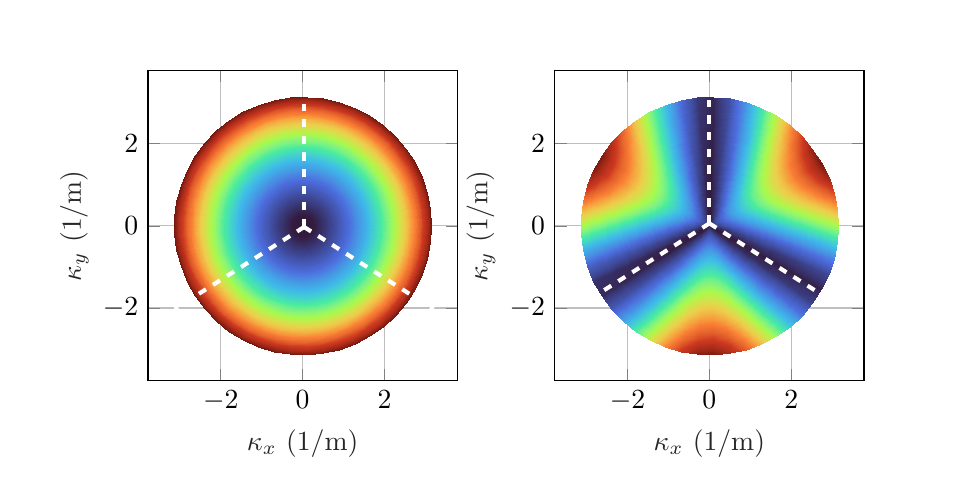
\begin{tikzpicture}

\begin{axis}[%
width=0.324\textwidth,
height=0.325\textwidth,
at={(0\textwidth,0\textwidth)},
scale only axis,
xmin=-3.77645049743461,
xmax=3.77645049743461,
xlabel style={font=\color{white!15!black}},
xlabel={$\kappa_x$ (1/m)},
ymin=-3.77645049743461,
ymax=3.77645049743461,
ylabel style={font=\color{white!15!black}},
ylabel={$\kappa_y$ (1/m)},
axis background/.style={fill=white},
xmajorgrids,
ymajorgrids,
ylabel style={yshift=-1.75pt}
]

\addplot[%
surf,
shader=interp, colormap={mymap}{[1pt] rgb(0pt)=(0.2,0.1059,0.2431); rgb(1pt)=(0.2104,0.1627,0.3554); rgb(2pt)=(0.2202,0.204,0.4359); rgb(3pt)=(0.2295,0.2376,0.5013); rgb(4pt)=(0.2385,0.2666,0.5573); rgb(5pt)=(0.2471,0.2923,0.6069); rgb(6pt)=(0.2553,0.3156,0.6518); rgb(7pt)=(0.2633,0.337,0.6931); rgb(8pt)=(0.271,0.3569,0.7314); rgb(9pt)=(0.2784,0.3755,0.7672); rgb(10pt)=(0.2856,0.3931,0.801); rgb(11pt)=(0.2926,0.4097,0.833); rgb(12pt)=(0.2994,0.4256,0.8634); rgb(13pt)=(0.2993,0.4519,0.8765); rgb(14pt)=(0.295,0.4827,0.8798); rgb(15pt)=(0.2906,0.5111,0.883); rgb(16pt)=(0.2862,0.5377,0.8862); rgb(17pt)=(0.2817,0.5627,0.8894); rgb(18pt)=(0.277,0.5864,0.8926); rgb(19pt)=(0.2723,0.6089,0.8958); rgb(20pt)=(0.2675,0.6304,0.8989); rgb(21pt)=(0.2626,0.651,0.9021); rgb(22pt)=(0.2576,0.6707,0.9052); rgb(23pt)=(0.2524,0.6898,0.9083); rgb(24pt)=(0.2472,0.7082,0.9114); rgb(25pt)=(0.2441,0.7264,0.9089); rgb(26pt)=(0.2479,0.7455,0.8894); rgb(27pt)=(0.2516,0.764,0.8693); rgb(28pt)=(0.2553,0.782,0.8485); rgb(29pt)=(0.2589,0.7994,0.8271); rgb(30pt)=(0.2624,0.8163,0.8049); rgb(31pt)=(0.2659,0.8328,0.7819); rgb(32pt)=(0.2694,0.8488,0.7579); rgb(33pt)=(0.2728,0.8645,0.733); rgb(34pt)=(0.2761,0.8798,0.7068); rgb(35pt)=(0.2794,0.8947,0.6794); rgb(36pt)=(0.2827,0.9094,0.6504); rgb(37pt)=(0.2859,0.9237,0.6196); rgb(38pt)=(0.3296,0.9295,0.5999); rgb(39pt)=(0.3722,0.9341,0.5812); rgb(40pt)=(0.4095,0.9386,0.5616); rgb(41pt)=(0.4431,0.9431,0.5412); rgb(42pt)=(0.4737,0.9476,0.5197); rgb(43pt)=(0.5021,0.9521,0.4971); rgb(44pt)=(0.5285,0.9565,0.4731); rgb(45pt)=(0.5534,0.9609,0.4474); rgb(46pt)=(0.5769,0.9653,0.4198); rgb(47pt)=(0.5993,0.9696,0.3897); rgb(48pt)=(0.6206,0.974,0.3564); rgb(49pt)=(0.6411,0.9783,0.3189); rgb(50pt)=(0.6653,0.9741,0.2979); rgb(51pt)=(0.6928,0.9612,0.2976); rgb(52pt)=(0.7189,0.9482,0.2973); rgb(53pt)=(0.7438,0.9349,0.2969); rgb(54pt)=(0.7677,0.9214,0.2966); rgb(55pt)=(0.7907,0.9075,0.2963); rgb(56pt)=(0.8128,0.8934,0.296); rgb(57pt)=(0.8342,0.879,0.2957); rgb(58pt)=(0.8549,0.8643,0.2954); rgb(59pt)=(0.8749,0.8493,0.295); rgb(60pt)=(0.8944,0.8339,0.2947); rgb(61pt)=(0.9133,0.8181,0.2944); rgb(62pt)=(0.9299,0.8016,0.2934); rgb(63pt)=(0.9342,0.7825,0.2875); rgb(64pt)=(0.9384,0.7628,0.2815); rgb(65pt)=(0.9426,0.7424,0.2753); rgb(66pt)=(0.9468,0.7213,0.2689); rgb(67pt)=(0.951,0.6993,0.2624); rgb(68pt)=(0.9551,0.6764,0.2556); rgb(69pt)=(0.9592,0.6525,0.2487); rgb(70pt)=(0.9633,0.6273,0.2415); rgb(71pt)=(0.9673,0.6008,0.2341); rgb(72pt)=(0.9714,0.5726,0.2264); rgb(73pt)=(0.9754,0.5426,0.2183); rgb(74pt)=(0.9794,0.5103,0.21); rgb(75pt)=(0.9712,0.4904,0.204); rgb(76pt)=(0.9589,0.4744,0.1987); rgb(77pt)=(0.9463,0.4577,0.1933); rgb(78pt)=(0.9335,0.4402,0.1878); rgb(79pt)=(0.9205,0.4218,0.182); rgb(80pt)=(0.9072,0.4024,0.176); rgb(81pt)=(0.8936,0.3817,0.1699); rgb(82pt)=(0.8798,0.3596,0.1634); rgb(83pt)=(0.8657,0.3357,0.1567); rgb(84pt)=(0.8513,0.3095,0.1497); rgb(85pt)=(0.8365,0.2803,0.1423); rgb(86pt)=(0.8214,0.247,0.1345); rgb(87pt)=(0.8039,0.2207,0.1277); rgb(88pt)=(0.7824,0.2131,0.1232); rgb(89pt)=(0.76,0.2051,0.1185); rgb(90pt)=(0.7368,0.1967,0.1136); rgb(91pt)=(0.7126,0.188,0.1084); rgb(92pt)=(0.6873,0.1787,0.1031); rgb(93pt)=(0.6607,0.169,0.0975); rgb(94pt)=(0.6327,0.1586,0.0915); rgb(95pt)=(0.603,0.1474,0.0853); rgb(96pt)=(0.5712,0.1353,0.0786); rgb(97pt)=(0.537,0.122,0.0714); rgb(98pt)=(0.4999,0.1072,0.0635); rgb(99pt)=(0.4588,0.0902,0.0549)}, mesh/rows=50]
table[row sep=crcr, point meta=\thisrow{c}] {%
%
x	y	c\\
0	0	100\\
0.0641141357875468	0	100.000036708885\\
0.128228271575094	0	100.000146835527\\
0.19234240736264	0	100.000330379891\\
0.256456543150187	0	100.000587341917\\
0.320570678937734	0	100.00091772152\\
0.384684814725281	0	100.001321518594\\
0.448798950512828	0	100.001798733005\\
0.512913086300374	0	100.0023493646\\
0.577027222087921	0	100.002973413197\\
0.641141357875468	0	100.003670878594\\
0.705255493663015	0	100.004441760562\\
0.769369629450562	0	100.005286058851\\
0.833483765238108	0	100.006203773184\\
0.897597901025655	0	100.007194903263\\
0.961712036813202	0	100.008259448763\\
1.02582617260075	0	100.009397409337\\
1.0899403083883	0	100.010608784615\\
1.15405444417584	0	100.011893574201\\
1.21816857996339	0	100.013251777676\\
1.28228271575094	0	100.014683394596\\
1.34639685153848	0	100.016188424494\\
1.41051098732603	0	100.017766866879\\
1.47462512311358	0	100.019418721237\\
1.53873925890112	0	100.021143987028\\
1.60285339468867	0	100.02294266369\\
1.66696753047622	0	100.024814750635\\
1.73108166626376	0	100.026760247252\\
1.79519580205131	0	100.028779152908\\
1.85930993783886	0	100.030871466942\\
1.9234240736264	0	100.033037188673\\
1.98753820941395	0	100.035276317393\\
2.0516523452015	0	100.037588852373\\
2.11576648098904	0	100.039974792857\\
2.17988061677659	0	100.042434138068\\
2.24399475256414	0	100.044966887202\\
2.30810888835168	0	100.047573039433\\
2.37222302413923	0	100.050252593912\\
2.43633715992678	0	100.053005549763\\
2.50045129571433	0	100.055831906088\\
2.56456543150187	0	100.058731661966\\
2.62867956728942	0	100.061704816451\\
2.69279370307697	0	100.064751368571\\
2.75690783886451	0	100.067871317334\\
2.82102197465206	0	100.071064661721\\
2.88513611043961	0	100.07433140069\\
2.94925024622715	0	100.077671533176\\
3.0133643820147	0	100.081085058089\\
3.07747851780225	0	100.084571974315\\
3.14159265358979	0	100.088132280716\\
0	0	100\\
0.0635877596189965	0.00819873370836649	100.000036708885\\
0.127175519237993	0.016397467416733	100.000146835527\\
0.19076327885699	0.0245962011250995	100.000330379891\\
0.254351038475986	0.032794934833466	100.000587341917\\
0.317938798094983	0.0409936685418325	100.00091772152\\
0.381526557713979	0.049192402250199	100.001321518594\\
0.445114317332976	0.0573911359585655	100.001798733005\\
0.508702076951972	0.0655898696669319	100.0023493646\\
0.572289836570969	0.0737886033752985	100.002973413197\\
0.635877596189965	0.0819873370836649	100.003670878594\\
0.699465355808962	0.0901860707920314	100.004441760562\\
0.763053115427958	0.0983848045003979	100.005286058851\\
0.826640875046955	0.106583538208764	100.006203773184\\
0.890228634665951	0.114782271917131	100.007194903263\\
0.953816394284948	0.122981005625497	100.008259448763\\
1.01740415390394	0.131179739333864	100.009397409337\\
1.08099191352294	0.13937847304223	100.010608784615\\
1.14457967314194	0.147577206750597	100.011893574201\\
1.20816743276093	0.155775940458963	100.013251777676\\
1.27175519237993	0.16397467416733	100.014683394596\\
1.33534295199893	0.172173407875696	100.016188424494\\
1.39893071161792	0.180372141584063	100.017766866879\\
1.46251847123692	0.188570875292429	100.019418721237\\
1.52610623085592	0.196769609000796	100.021143987028\\
1.58969399047491	0.204968342709162	100.02294266369\\
1.65328175009391	0.213167076417529	100.024814750635\\
1.71686950971291	0.221365810125895	100.026760247252\\
1.7804572693319	0.229564543834262	100.028779152908\\
1.8440450289509	0.237763277542628	100.030871466942\\
1.9076327885699	0.245962011250995	100.033037188673\\
1.97122054818889	0.254160744959361	100.035276317393\\
2.03480830780789	0.262359478667728	100.037588852373\\
2.09839606742689	0.270558212376094	100.039974792857\\
2.16198382704588	0.278756946084461	100.042434138068\\
2.22557158666488	0.286955679792827	100.044966887202\\
2.28915934628388	0.295154413501194	100.047573039433\\
2.35274710590287	0.30335314720956	100.050252593912\\
2.41633486552187	0.311551880917927	100.053005549763\\
2.47992262514086	0.319750614626293	100.055831906088\\
2.54351038475986	0.32794934833466	100.058731661966\\
2.60709814437886	0.336148082043026	100.061704816451\\
2.67068590399785	0.344346815751393	100.064751368571\\
2.73427366361685	0.352545549459759	100.067871317334\\
2.79786142323585	0.360744283168126	100.071064661721\\
2.86144918285484	0.368943016876492	100.07433140069\\
2.92503694247384	0.377141750584859	100.077671533176\\
2.98862470209284	0.385340484293225	100.081085058089\\
3.05221246171183	0.393539218001592	100.084571974315\\
3.11580022133083	0.401737951709958	100.088132280716\\
0	0	100\\
0.0620172741954808	0.0162628444359078	100.000036708885\\
0.124034548390962	0.0325256888718157	100.000146835527\\
0.186051822586442	0.0487885333077235	100.000330379891\\
0.248069096781923	0.0650513777436313	100.000587341917\\
0.310086370977404	0.0813142221795392	100.00091772152\\
0.372103645172885	0.097577066615447	100.001321518594\\
0.434120919368366	0.113839911051355	100.001798733005\\
0.496138193563847	0.130102755487263	100.0023493646\\
0.558155467759327	0.146365599923171	100.002973413197\\
0.620172741954808	0.162628444359078	100.003670878594\\
0.682190016150289	0.178891288794986	100.004441760562\\
0.74420729034577	0.195154133230894	100.005286058851\\
0.806224564541251	0.211416977666802	100.006203773184\\
0.868241838736731	0.22767982210271	100.007194903263\\
0.930259112932212	0.243942666538618	100.008259448763\\
0.992276387127693	0.260205510974525	100.009397409337\\
1.05429366132317	0.276468355410433	100.010608784615\\
1.11631093551865	0.292731199846341	100.011893574201\\
1.17832820971414	0.308994044282249	100.013251777676\\
1.24034548390962	0.325256888718157	100.014683394596\\
1.3023627581051	0.341519733154065	100.016188424494\\
1.36438003230058	0.357782577589972	100.017766866879\\
1.42639730649606	0.37404542202588	100.019418721237\\
1.48841458069154	0.390308266461788	100.021143987028\\
1.55043185488702	0.406571110897696	100.02294266369\\
1.6124491290825	0.422833955333604	100.024814750635\\
1.67446640327798	0.439096799769512	100.026760247252\\
1.73648367747346	0.455359644205419	100.028779152908\\
1.79850095166894	0.471622488641327	100.030871466942\\
1.86051822586442	0.487885333077235	100.033037188673\\
1.92253550005991	0.504148177513143	100.035276317393\\
1.98455277425539	0.520411021949051	100.037588852373\\
2.04657004845087	0.536673866384959	100.039974792857\\
2.10858732264635	0.552936710820866	100.042434138068\\
2.17060459684183	0.569199555256774	100.044966887202\\
2.23262187103731	0.585462399692682	100.047573039433\\
2.29463914523279	0.60172524412859	100.050252593912\\
2.35665641942827	0.617988088564498	100.053005549763\\
2.41867369362375	0.634250933000406	100.055831906088\\
2.48069096781923	0.650513777436314	100.058731661966\\
2.54270824201471	0.666776621872221	100.061704816451\\
2.60472551621019	0.683039466308129	100.064751368571\\
2.66674279040567	0.699302310744037	100.067871317334\\
2.72876006460116	0.715565155179945	100.071064661721\\
2.79077733879664	0.731827999615853	100.07433140069\\
2.85279461299212	0.748090844051761	100.077671533176\\
2.9148118871876	0.764353688487668	100.081085058089\\
2.97682916138308	0.780616532923576	100.084571974315\\
3.03884643557856	0.796879377359484	100.088132280716\\
0	0	100\\
0.0594284668442354	0.0240599197074222	100.000036708885\\
0.118856933688471	0.0481198394148444	100.000146835527\\
0.178285400532706	0.0721797591222665	100.000330379891\\
0.237713867376942	0.0962396788296887	100.000587341917\\
0.297142334221177	0.120299598537111	100.00091772152\\
0.356570801065412	0.144359518244533	100.001321518594\\
0.415999267909648	0.168419437951955	100.001798733005\\
0.475427734753883	0.192479357659377	100.0023493646\\
0.534856201598119	0.2165392773668	100.002973413197\\
0.594284668442354	0.240599197074222	100.003670878594\\
0.653713135286589	0.264659116781644	100.004441760562\\
0.713141602130825	0.288719036489066	100.005286058851\\
0.77257006897506	0.312778956196488	100.006203773184\\
0.831998535819296	0.33683887590391	100.007194903263\\
0.891427002663531	0.360898795611333	100.008259448763\\
0.950855469507766	0.384958715318755	100.009397409337\\
1.010283936352	0.409018635026177	100.010608784615\\
1.06971240319624	0.433078554733599	100.011893574201\\
1.12914087004047	0.457138474441021	100.013251777676\\
1.18856933688471	0.481198394148444	100.014683394596\\
1.24799780372894	0.505258313855866	100.016188424494\\
1.30742627057318	0.529318233563288	100.017766866879\\
1.36685473741741	0.55337815327071	100.019418721237\\
1.42628320426165	0.577438072978132	100.021143987028\\
1.48571167110589	0.601497992685554	100.02294266369\\
1.54514013795012	0.625557912392977	100.024814750635\\
1.60456860479436	0.649617832100399	100.026760247252\\
1.66399707163859	0.673677751807821	100.028779152908\\
1.72342553848283	0.697737671515243	100.030871466942\\
1.78285400532706	0.721797591222665	100.033037188673\\
1.8422824721713	0.745857510930087	100.035276317393\\
1.90171093901553	0.76991743063751	100.037588852373\\
1.96113940585977	0.793977350344932	100.039974792857\\
2.020567872704	0.818037270052354	100.042434138068\\
2.07999633954824	0.842097189759776	100.044966887202\\
2.13942480639247	0.866157109467198	100.047573039433\\
2.19885327323671	0.890217029174621	100.050252593912\\
2.25828174008095	0.914276948882043	100.053005549763\\
2.31771020692518	0.938336868589465	100.055831906088\\
2.37713867376942	0.962396788296887	100.058731661966\\
2.43656714061365	0.986456708004309	100.061704816451\\
2.49599560745789	1.01051662771173	100.064751368571\\
2.55542407430212	1.03457654741915	100.067871317334\\
2.61485254114636	1.05863646712658	100.071064661721\\
2.67428100799059	1.082696386834	100.07433140069\\
2.73370947483483	1.10675630654142	100.077671533176\\
2.79313794167906	1.13081622624884	100.081085058089\\
2.8525664085233	1.15487614595626	100.084571974315\\
2.91199487536753	1.17893606566369	100.088132280716\\
0	0	100\\
0.0558638457103963	0.031461931762513	100.000036708885\\
0.111727691420793	0.062923863525026	100.000146835527\\
0.167591537131189	0.0943857952875391	100.000330379891\\
0.223455382841585	0.125847727050052	100.000587341917\\
0.279319228551981	0.157309658812565	100.00091772152\\
0.335183074262378	0.188771590575078	100.001321518594\\
0.391046919972774	0.220233522337591	100.001798733005\\
0.44691076568317	0.251695454100104	100.0023493646\\
0.502774611393567	0.283157385862617	100.002973413197\\
0.558638457103963	0.31461931762513	100.003670878594\\
0.614502302814359	0.346081249387643	100.004441760562\\
0.670366148524756	0.377543181150156	100.005286058851\\
0.726229994235152	0.409005112912669	100.006203773184\\
0.782093839945548	0.440467044675182	100.007194903263\\
0.837957685655945	0.471928976437695	100.008259448763\\
0.893821531366341	0.503390908200208	100.009397409337\\
0.949685377076737	0.534852839962722	100.010608784615\\
1.00554922278713	0.566314771725235	100.011893574201\\
1.06141306849753	0.597776703487747	100.013251777676\\
1.11727691420793	0.629238635250261	100.014683394596\\
1.17314075991832	0.660700567012774	100.016188424494\\
1.22900460562872	0.692162498775286	100.017766866879\\
1.28486845133911	0.7236244305378	100.019418721237\\
1.34073229704951	0.755086362300313	100.021143987028\\
1.39659614275991	0.786548294062826	100.02294266369\\
1.4524599884703	0.818010225825339	100.024814750635\\
1.5083238341807	0.849472157587852	100.026760247252\\
1.5641876798911	0.880934089350365	100.028779152908\\
1.62005152560149	0.912396021112878	100.030871466942\\
1.67591537131189	0.943857952875391	100.033037188673\\
1.73177921702229	0.975319884637904	100.035276317393\\
1.78764306273268	1.00678181640042	100.037588852373\\
1.84350690844308	1.03824374816293	100.039974792857\\
1.89937075415347	1.06970567992544	100.042434138068\\
1.95523459986387	1.10116761168796	100.044966887202\\
2.01109844557427	1.13262954345047	100.047573039433\\
2.06696229128466	1.16409147521298	100.050252593912\\
2.12282613699506	1.19555340697549	100.053005549763\\
2.17868998270546	1.22701533873801	100.055831906088\\
2.23455382841585	1.25847727050052	100.058731661966\\
2.29041767412625	1.28993920226303	100.061704816451\\
2.34628151983664	1.32140113402555	100.064751368571\\
2.40214536554704	1.35286306578806	100.067871317334\\
2.45800921125744	1.38432499755057	100.071064661721\\
2.51387305696783	1.41578692931309	100.07433140069\\
2.56973690267823	1.4472488610756	100.077671533176\\
2.62560074838863	1.47871079283811	100.081085058089\\
2.68146459409902	1.51017272460063	100.084571974315\\
2.73732843980942	1.54163465636314	100.088132280716\\
0	0	100\\
0.0513819417744319	0.0383473397678755	100.000036708885\\
0.102763883548864	0.0766946795357509	100.000146835527\\
0.154145825323296	0.115042019303626	100.000330379891\\
0.205527767097727	0.153389359071502	100.000587341917\\
0.256909708872159	0.191736698839377	100.00091772152\\
0.308291650646591	0.230084038607253	100.001321518594\\
0.359673592421023	0.268431378375128	100.001798733005\\
0.411055534195455	0.306778718143004	100.0023493646\\
0.462437475969887	0.345126057910879	100.002973413197\\
0.513819417744319	0.383473397678755	100.003670878594\\
0.56520135951875	0.42182073744663	100.004441760562\\
0.616583301293182	0.460168077214506	100.005286058851\\
0.667965243067614	0.498515416982381	100.006203773184\\
0.719347184842046	0.536862756750257	100.007194903263\\
0.770729126616478	0.575210096518132	100.008259448763\\
0.82211106839091	0.613557436286007	100.009397409337\\
0.873493010165342	0.651904776053883	100.010608784615\\
0.924874951939773	0.690252115821758	100.011893574201\\
0.976256893714205	0.728599455589634	100.013251777676\\
1.02763883548864	0.766946795357509	100.014683394596\\
1.07902077726307	0.805294135125385	100.016188424494\\
1.1304027190375	0.84364147489326	100.017766866879\\
1.18178466081193	0.881988814661136	100.019418721237\\
1.23316660258636	0.920336154429011	100.021143987028\\
1.2845485443608	0.958683494196887	100.02294266369\\
1.33593048613523	0.997030833964762	100.024814750635\\
1.38731242790966	1.03537817373264	100.026760247252\\
1.43869436968409	1.07372551350051	100.028779152908\\
1.49007631145852	1.11207285326839	100.030871466942\\
1.54145825323296	1.15042019303626	100.033037188673\\
1.59284019500739	1.18876753280414	100.035276317393\\
1.64422213678182	1.22711487257201	100.037588852373\\
1.69560407855625	1.26546221233989	100.039974792857\\
1.74698602033068	1.30380955210777	100.042434138068\\
1.79836796210511	1.34215689187564	100.044966887202\\
1.84974990387955	1.38050423164352	100.047573039433\\
1.90113184565398	1.41885157141139	100.050252593912\\
1.95251378742841	1.45719891117927	100.053005549763\\
2.00389572920284	1.49554625094714	100.055831906088\\
2.05527767097727	1.53389359071502	100.058731661966\\
2.10665961275171	1.57224093048289	100.061704816451\\
2.15804155452614	1.61058827025077	100.064751368571\\
2.20942349630057	1.64893561001865	100.067871317334\\
2.260805438075	1.68728294978652	100.071064661721\\
2.31218737984943	1.7256302895544	100.07433140069\\
2.36356932162387	1.76397762932227	100.077671533176\\
2.4149512633983	1.80232496909015	100.081085058089\\
2.46633320517273	1.84067230885802	100.084571974315\\
2.51771514694716	1.8790196486259	100.088132280716\\
0	0	100\\
0.0460563477750617	0.0446030855144188	100.000036708885\\
0.0921126955501234	0.0892061710288376	100.000146835527\\
0.138169043325185	0.133809256543256	100.000330379891\\
0.184225391100247	0.178412342057675	100.000587341917\\
0.230281738875309	0.223015427572094	100.00091772152\\
0.27633808665037	0.267618513086513	100.001321518594\\
0.322394434425432	0.312221598600932	100.001798733005\\
0.368450782200494	0.356824684115351	100.0023493646\\
0.414507129975555	0.401427769629769	100.002973413197\\
0.460563477750617	0.446030855144188	100.003670878594\\
0.506619825525679	0.490633940658607	100.004441760562\\
0.55267617330074	0.535237026173026	100.005286058851\\
0.598732521075802	0.579840111687445	100.006203773184\\
0.644788868850864	0.624443197201863	100.007194903263\\
0.690845216625925	0.669046282716282	100.008259448763\\
0.736901564400987	0.713649368230701	100.009397409337\\
0.782957912176049	0.75825245374512	100.010608784615\\
0.829014259951111	0.802855539259539	100.011893574201\\
0.875070607726172	0.847458624773958	100.013251777676\\
0.921126955501234	0.892061710288376	100.014683394596\\
0.967183303276296	0.936664795802795	100.016188424494\\
1.01323965105136	0.981267881317214	100.017766866879\\
1.05929599882642	1.02587096683163	100.019418721237\\
1.10535234660148	1.07047405234605	100.021143987028\\
1.15140869437654	1.11507713786047	100.02294266369\\
1.1974650421516	1.15968022337489	100.024814750635\\
1.24352138992667	1.20428330888931	100.026760247252\\
1.28957773770173	1.24888639440373	100.028779152908\\
1.33563408547679	1.29348947991815	100.030871466942\\
1.38169043325185	1.33809256543256	100.033037188673\\
1.42774678102691	1.38269565094698	100.035276317393\\
1.47380312880197	1.4272987364614	100.037588852373\\
1.51985947657704	1.47190182197582	100.039974792857\\
1.5659158243521	1.51650490749024	100.042434138068\\
1.61197217212716	1.56110799300466	100.044966887202\\
1.65802851990222	1.60571107851908	100.047573039433\\
1.70408486767728	1.6503141640335	100.050252593912\\
1.75014121545234	1.69491724954792	100.053005549763\\
1.79619756322741	1.73952033506233	100.055831906088\\
1.84225391100247	1.78412342057675	100.058731661966\\
1.88831025877753	1.82872650609117	100.061704816451\\
1.93436660655259	1.87332959160559	100.064751368571\\
1.98042295432765	1.91793267712001	100.067871317334\\
2.02647930210271	1.96253576263443	100.071064661721\\
2.07253564987778	2.00713884814885	100.07433140069\\
2.11859199765284	2.05174193366327	100.077671533176\\
2.1646483454279	2.09634501917768	100.081085058089\\
2.21070469320296	2.1409481046921	100.084571974315\\
2.25676104097802	2.18555119020652	100.088132280716\\
0	0	100\\
0.0399745098185215	0.0501264498299343	100.000036708885\\
0.079949019637043	0.100252899659869	100.000146835527\\
0.119923529455564	0.150379349489803	100.000330379891\\
0.159898039274086	0.200505799319737	100.000587341917\\
0.199872549092607	0.250632249149671	100.00091772152\\
0.239847058911129	0.300758698979606	100.001321518594\\
0.27982156872965	0.35088514880954	100.001798733005\\
0.319796078548172	0.401011598639474	100.0023493646\\
0.359770588366693	0.451138048469409	100.002973413197\\
0.399745098185215	0.501264498299343	100.003670878594\\
0.439719608003736	0.551390948129277	100.004441760562\\
0.479694117822258	0.601517397959211	100.005286058851\\
0.519668627640779	0.651643847789146	100.006203773184\\
0.559643137459301	0.70177029761908	100.007194903263\\
0.599617647277822	0.751896747449014	100.008259448763\\
0.639592157096344	0.802023197278948	100.009397409337\\
0.679566666914865	0.852149647108883	100.010608784615\\
0.719541176733387	0.902276096938817	100.011893574201\\
0.759515686551908	0.952402546768751	100.013251777676\\
0.79949019637043	1.00252899659869	100.014683394596\\
0.839464706188951	1.05265544642862	100.016188424494\\
0.879439216007473	1.10278189625855	100.017766866879\\
0.919413725825994	1.15290834608849	100.019418721237\\
0.959388235644516	1.20303479591842	100.021143987028\\
0.999362745463037	1.25316124574836	100.02294266369\\
1.03933725528156	1.30328769557829	100.024814750635\\
1.07931176510008	1.35341414540823	100.026760247252\\
1.1192862749186	1.40354059523816	100.028779152908\\
1.15926078473712	1.45366704506809	100.030871466942\\
1.19923529455564	1.50379349489803	100.033037188673\\
1.23920980437417	1.55391994472796	100.035276317393\\
1.27918431419269	1.6040463945579	100.037588852373\\
1.31915882401121	1.65417284438783	100.039974792857\\
1.35913333382973	1.70429929421777	100.042434138068\\
1.39910784364825	1.7544257440477	100.044966887202\\
1.43908235346677	1.80455219387763	100.047573039433\\
1.4790568632853	1.85467864370757	100.050252593912\\
1.51903137310382	1.9048050935375	100.053005549763\\
1.55900588292234	1.95493154336744	100.055831906088\\
1.59898039274086	2.00505799319737	100.058731661966\\
1.63895490255938	2.05518444302731	100.061704816451\\
1.6789294123779	2.10531089285724	100.064751368571\\
1.71890392219642	2.15543734268717	100.067871317334\\
1.75887843201495	2.20556379251711	100.071064661721\\
1.79885294183347	2.25569024234704	100.07433140069\\
1.83882745165199	2.30581669217698	100.077671533176\\
1.87880196147051	2.35594314200691	100.081085058089\\
1.91877647128903	2.40606959183685	100.084571974315\\
1.95875098110755	2.45619604166678	100.088132280716\\
0	0	100\\
0.0332362915159161	0.0548267392250627	100.000036708885\\
0.0664725830318323	0.109653478450125	100.000146835527\\
0.0997088745477484	0.164480217675188	100.000330379891\\
0.132945166063665	0.219306956900251	100.000587341917\\
0.166181457579581	0.274133696125314	100.00091772152\\
0.199417749095497	0.328960435350376	100.001321518594\\
0.232654040611413	0.383787174575439	100.001798733005\\
0.265890332127329	0.438613913800502	100.0023493646\\
0.299126623643245	0.493440653025564	100.002973413197\\
0.332362915159161	0.548267392250627	100.003670878594\\
0.365599206675077	0.60309413147569	100.004441760562\\
0.398835498190994	0.657920870700752	100.005286058851\\
0.43207178970691	0.712747609925815	100.006203773184\\
0.465308081222826	0.767574349150878	100.007194903263\\
0.498544372738742	0.822401088375941	100.008259448763\\
0.531780664254658	0.877227827601003	100.009397409337\\
0.565016955770574	0.932054566826066	100.010608784615\\
0.598253247286491	0.986881306051129	100.011893574201\\
0.631489538802407	1.04170804527619	100.013251777676\\
0.664725830318323	1.09653478450125	100.014683394596\\
0.697962121834239	1.15136152372632	100.016188424494\\
0.731198413350155	1.20618826295138	100.017766866879\\
0.764434704866071	1.26101500217644	100.019418721237\\
0.797670996381987	1.3158417414015	100.021143987028\\
0.830907287897904	1.37066848062657	100.02294266369\\
0.86414357941382	1.42549521985163	100.024814750635\\
0.897379870929736	1.48032195907669	100.026760247252\\
0.930616162445652	1.53514869830176	100.028779152908\\
0.963852453961568	1.58997543752682	100.030871466942\\
0.997088745477484	1.64480217675188	100.033037188673\\
1.0303250369934	1.69962891597694	100.035276317393\\
1.06356132850932	1.75445565520201	100.037588852373\\
1.09679762002523	1.80928239442707	100.039974792857\\
1.13003391154115	1.86410913365213	100.042434138068\\
1.16327020305706	1.91893587287719	100.044966887202\\
1.19650649457298	1.97376261210226	100.047573039433\\
1.2297427860889	2.02858935132732	100.050252593912\\
1.26297907760481	2.08341609055238	100.053005549763\\
1.29621536912073	2.13824282977745	100.055831906088\\
1.32945166063665	2.19306956900251	100.058731661966\\
1.36268795215256	2.24789630822757	100.061704816451\\
1.39592424366848	2.30272304745263	100.064751368571\\
1.42916053518439	2.3575497866777	100.067871317334\\
1.46239682670031	2.41237652590276	100.071064661721\\
1.49563311821623	2.46720326512782	100.07433140069\\
1.52886940973214	2.52203000435288	100.077671533176\\
1.56210570124806	2.57685674357795	100.081085058089\\
1.59534199276397	2.63168348280301	100.084571974315\\
1.62857828427989	2.68651022202807	100.088132280716\\
0	0	100\\
0.0259523342254863	0.0586267750778826	100.000036708885\\
0.0519046684509726	0.117253550155765	100.000146835527\\
0.0778570026764589	0.175880325233648	100.000330379891\\
0.103809336901945	0.234507100311531	100.000587341917\\
0.129761671127432	0.293133875389413	100.00091772152\\
0.155714005352918	0.351760650467296	100.001321518594\\
0.181666339578404	0.410387425545178	100.001798733005\\
0.20761867380389	0.469014200623061	100.0023493646\\
0.233571008029377	0.527640975700944	100.002973413197\\
0.259523342254863	0.586267750778826	100.003670878594\\
0.285475676480349	0.644894525856709	100.004441760562\\
0.311428010705836	0.703521300934592	100.005286058851\\
0.337380344931322	0.762148076012474	100.006203773184\\
0.363332679156808	0.820774851090357	100.007194903263\\
0.389285013382295	0.87940162616824	100.008259448763\\
0.415237347607781	0.938028401246122	100.009397409337\\
0.441189681833267	0.996655176324005	100.010608784615\\
0.467142016058753	1.05528195140189	100.011893574201\\
0.49309435028424	1.11390872647977	100.013251777676\\
0.519046684509726	1.17253550155765	100.014683394596\\
0.544999018735212	1.23116227663554	100.016188424494\\
0.570951352960699	1.28978905171342	100.017766866879\\
0.596903687186185	1.3484158267913	100.019418721237\\
0.622856021411671	1.40704260186918	100.021143987028\\
0.648808355637158	1.46566937694707	100.02294266369\\
0.674760689862644	1.52429615202495	100.024814750635\\
0.70071302408813	1.58292292710283	100.026760247252\\
0.726665358313616	1.64154970218071	100.028779152908\\
0.752617692539103	1.7001764772586	100.030871466942\\
0.778570026764589	1.75880325233648	100.033037188673\\
0.804522360990075	1.81743002741436	100.035276317393\\
0.830474695215562	1.87605680249224	100.037588852373\\
0.856427029441048	1.93468357757013	100.039974792857\\
0.882379363666534	1.99331035264801	100.042434138068\\
0.908331697892021	2.05193712772589	100.044966887202\\
0.934284032117507	2.11056390280378	100.047573039433\\
0.960236366342993	2.16919067788166	100.050252593912\\
0.986188700568479	2.22781745295954	100.053005549763\\
1.01214103479397	2.28644422803742	100.055831906088\\
1.03809336901945	2.34507100311531	100.058731661966\\
1.06404570324494	2.40369777819319	100.061704816451\\
1.08999803747042	2.46232455327107	100.064751368571\\
1.11595037169591	2.52095132834895	100.067871317334\\
1.1419027059214	2.57957810342684	100.071064661721\\
1.16785504014688	2.63820487850472	100.07433140069\\
1.19380737437237	2.6968316535826	100.077671533176\\
1.21975970859786	2.75545842866048	100.081085058089\\
1.24571204282334	2.81408520373837	100.084571974315\\
1.27166437704883	2.87271197881625	100.088132280716\\
0	0	100\\
0.018242240324565	0.0614641609047484	100.000036708885\\
0.03648448064913	0.122928321809497	100.000146835527\\
0.054726720973695	0.184392482714245	100.000330379891\\
0.07296896129826	0.245856643618994	100.000587341917\\
0.091211201622825	0.307320804523742	100.00091772152\\
0.10945344194739	0.36878496542849	100.001321518594\\
0.127695682271955	0.430249126333239	100.001798733005\\
0.14593792259652	0.491713287237987	100.0023493646\\
0.164180162921085	0.553177448142736	100.002973413197\\
0.18242240324565	0.614641609047484	100.003670878594\\
0.200664643570215	0.676105769952232	100.004441760562\\
0.21890688389478	0.737569930856981	100.005286058851\\
0.237149124219345	0.799034091761729	100.006203773184\\
0.25539136454391	0.860498252666478	100.007194903263\\
0.273633604868475	0.921962413571226	100.008259448763\\
0.29187584519304	0.983426574475975	100.009397409337\\
0.310118085517605	1.04489073538072	100.010608784615\\
0.32836032584217	1.10635489628547	100.011893574201\\
0.346602566166735	1.16781905719022	100.013251777676\\
0.3648448064913	1.22928321809497	100.014683394596\\
0.383087046815865	1.29074737899972	100.016188424494\\
0.40132928714043	1.35221153990446	100.017766866879\\
0.419571527464995	1.41367570080921	100.019418721237\\
0.43781376778956	1.47513986171396	100.021143987028\\
0.456056008114125	1.53660402261871	100.02294266369\\
0.47429824843869	1.59806818352346	100.024814750635\\
0.492540488763255	1.65953234442821	100.026760247252\\
0.51078272908782	1.72099650533296	100.028779152908\\
0.529024969412385	1.7824606662377	100.030871466942\\
0.54726720973695	1.84392482714245	100.033037188673\\
0.565509450061515	1.9053889880472	100.035276317393\\
0.58375169038608	1.96685314895195	100.037588852373\\
0.601993930710645	2.0283173098567	100.039974792857\\
0.62023617103521	2.08978147076145	100.042434138068\\
0.638478411359775	2.15124563166619	100.044966887202\\
0.65672065168434	2.21270979257094	100.047573039433\\
0.674962892008905	2.27417395347569	100.050252593912\\
0.69320513233347	2.33563811438044	100.053005549763\\
0.711447372658035	2.39710227528519	100.055831906088\\
0.7296896129826	2.45856643618994	100.058731661966\\
0.747931853307165	2.52003059709469	100.061704816451\\
0.76617409363173	2.58149475799943	100.064751368571\\
0.784416333956295	2.64295891890418	100.067871317334\\
0.80265857428086	2.70442307980893	100.071064661721\\
0.820900814605425	2.76588724071368	100.07433140069\\
0.83914305492999	2.82735140161843	100.077671533176\\
0.857385295254555	2.88881556252318	100.081085058089\\
0.87562753557912	2.95027972342792	100.084571974315\\
0.893869775903685	3.01174388433267	100.088132280716\\
0	0	100\\
0.0102326093418483	0.0632923069088267	100.000036708885\\
0.0204652186836966	0.126584613817653	100.000146835527\\
0.0306978280255449	0.18987692072648	100.000330379891\\
0.0409304373673932	0.253169227635307	100.000587341917\\
0.0511630467092416	0.316461534544133	100.00091772152\\
0.0613956560510899	0.37975384145296	100.001321518594\\
0.0716282653929382	0.443046148361787	100.001798733005\\
0.0818608747347865	0.506338455270613	100.0023493646\\
0.0920934840766348	0.56963076217944	100.002973413197\\
0.102326093418483	0.632923069088267	100.003670878594\\
0.112558702760331	0.696215375997093	100.004441760562\\
0.12279131210218	0.75950768290592	100.005286058851\\
0.133023921444028	0.822799989814747	100.006203773184\\
0.143256530785876	0.886092296723573	100.007194903263\\
0.153489140127725	0.9493846036324	100.008259448763\\
0.163721749469573	1.01267691054123	100.009397409337\\
0.173954358811421	1.07596921745005	100.010608784615\\
0.18418696815327	1.13926152435888	100.011893574201\\
0.194419577495118	1.20255383126771	100.013251777676\\
0.204652186836966	1.26584613817653	100.014683394596\\
0.214884796178815	1.32913844508536	100.016188424494\\
0.225117405520663	1.39243075199419	100.017766866879\\
0.235350014862511	1.45572305890301	100.019418721237\\
0.245582624204359	1.51901536581184	100.021143987028\\
0.255815233546208	1.58230767272067	100.02294266369\\
0.266047842888056	1.64559997962949	100.024814750635\\
0.276280452229904	1.70889228653832	100.026760247252\\
0.286513061571753	1.77218459344715	100.028779152908\\
0.296745670913601	1.83547690035597	100.030871466942\\
0.306978280255449	1.8987692072648	100.033037188673\\
0.317210889597298	1.96206151417363	100.035276317393\\
0.327443498939146	2.02535382108245	100.037588852373\\
0.337676108280994	2.08864612799128	100.039974792857\\
0.347908717622843	2.15193843490011	100.042434138068\\
0.358141326964691	2.21523074180893	100.044966887202\\
0.368373936306539	2.27852304871776	100.047573039433\\
0.378606545648388	2.34181535562659	100.050252593912\\
0.388839154990236	2.40510766253541	100.053005549763\\
0.399071764332084	2.46839996944424	100.055831906088\\
0.409304373673932	2.53169227635307	100.058731661966\\
0.419536983015781	2.59498458326189	100.061704816451\\
0.429769592357629	2.65827689017072	100.064751368571\\
0.440002201699477	2.72156919707955	100.067871317334\\
0.450234811041326	2.78486150398837	100.071064661721\\
0.460467420383174	2.8481538108972	100.07433140069\\
0.470700029725022	2.91144611780603	100.077671533176\\
0.480932639066871	2.97473842471485	100.081085058089\\
0.491165248408719	3.03803073162368	100.084571974315\\
0.501397857750567	3.10132303853251	100.088132280716\\
0	0	100\\
0.0020549591966342	0.0640811949832722	100.000036708885\\
0.0041099183932684	0.128162389966544	100.000146835527\\
0.0061648775899026	0.192243584949817	100.000330379891\\
0.0082198367865368	0.256324779933089	100.000587341917\\
0.010274795983171	0.320405974916361	100.00091772152\\
0.0123297551798052	0.384487169899634	100.001321518594\\
0.0143847143764394	0.448568364882906	100.001798733005\\
0.0164396735730736	0.512649559866178	100.0023493646\\
0.0184946327697078	0.57673075484945	100.002973413197\\
0.020549591966342	0.640811949832723	100.003670878594\\
0.0226045511629762	0.704893144815995	100.004441760562\\
0.0246595103596104	0.768974339799267	100.005286058851\\
0.0267144695562446	0.833055534782539	100.006203773184\\
0.0287694287528788	0.897136729765812	100.007194903263\\
0.030824387949513	0.961217924749084	100.008259448763\\
0.0328793471461472	1.02529911973236	100.009397409337\\
0.0349343063427814	1.08938031471563	100.010608784615\\
0.0369892655394156	1.1534615096989	100.011893574201\\
0.0390442247360498	1.21754270468217	100.013251777676\\
0.041099183932684	1.28162389966545	100.014683394596\\
0.0431541431293182	1.34570509464872	100.016188424494\\
0.0452091023259524	1.40978628963199	100.017766866879\\
0.0472640615225866	1.47386748461526	100.019418721237\\
0.0493190207192208	1.53794867959853	100.021143987028\\
0.051373979915855	1.60202987458181	100.02294266369\\
0.0534289391124892	1.66611106956508	100.024814750635\\
0.0554838983091234	1.73019226454835	100.026760247252\\
0.0575388575057576	1.79427345953162	100.028779152908\\
0.0595938167023918	1.8583546545149	100.030871466942\\
0.061648775899026	1.92243584949817	100.033037188673\\
0.0637037350956602	1.98651704448144	100.035276317393\\
0.0657586942922944	2.05059823946471	100.037588852373\\
0.0678136534889286	2.11467943444798	100.039974792857\\
0.0698686126855628	2.17876062943126	100.042434138068\\
0.071923571882197	2.24284182441453	100.044966887202\\
0.0739785310788312	2.3069230193978	100.047573039433\\
0.0760334902754654	2.37100421438107	100.050252593912\\
0.0780884494720996	2.43508540936435	100.053005549763\\
0.0801434086687338	2.49916660434762	100.055831906088\\
0.082198367865368	2.56324779933089	100.058731661966\\
0.0842533270620022	2.62732899431416	100.061704816451\\
0.0863082862586364	2.69141018929743	100.064751368571\\
0.0883632454552706	2.75549138428071	100.067871317334\\
0.0904182046519048	2.81957257926398	100.071064661721\\
0.092473163848539	2.88365377424725	100.07433140069\\
0.0945281230451732	2.94773496923052	100.077671533176\\
0.0965830822418074	3.0118161642138	100.081085058089\\
0.0986380414384416	3.07589735919707	100.084571974315\\
0.100693000635076	3.13997855418034	100.088132280716\\
-0	0	100\\
-0.00615643332177623	0.0638178716077128	100.000036708885\\
-0.0123128666435525	0.127635743215426	100.000146835527\\
-0.0184692999653287	0.191453614823138	100.000330379891\\
-0.0246257332871049	0.255271486430851	100.000587341917\\
-0.0307821666088812	0.319089358038564	100.00091772152\\
-0.0369385999306574	0.382907229646277	100.001321518594\\
-0.0430950332524336	0.446725101253989	100.001798733005\\
-0.0492514665742099	0.510542972861702	100.0023493646\\
-0.0554078998959861	0.574360844469415	100.002973413197\\
-0.0615643332177623	0.638178716077128	100.003670878594\\
-0.0677207665395385	0.70199658768484	100.004441760562\\
-0.0738771998613148	0.765814459292553	100.005286058851\\
-0.080033633183091	0.829632330900266	100.006203773184\\
-0.0861900665048673	0.893450202507979	100.007194903263\\
-0.0923464998266435	0.957268074115692	100.008259448763\\
-0.0985029331484197	1.0210859457234	100.009397409337\\
-0.104659366470196	1.08490381733112	100.010608784615\\
-0.110815799791972	1.14872168893883	100.011893574201\\
-0.116972233113748	1.21253956054654	100.013251777676\\
-0.123128666435525	1.27635743215426	100.014683394596\\
-0.129285099757301	1.34017530376197	100.016188424494\\
-0.135441533079077	1.40399317536968	100.017766866879\\
-0.141597966400853	1.46781104697739	100.019418721237\\
-0.14775439972263	1.53162891858511	100.021143987028\\
-0.153910833044406	1.59544679019282	100.02294266369\\
-0.160067266366182	1.65926466180053	100.024814750635\\
-0.166223699687958	1.72308253340824	100.026760247252\\
-0.172380133009735	1.78690040501596	100.028779152908\\
-0.178536566331511	1.85071827662367	100.030871466942\\
-0.184692999653287	1.91453614823138	100.033037188673\\
-0.190849432975063	1.9783540198391	100.035276317393\\
-0.197005866296839	2.04217189144681	100.037588852373\\
-0.203162299618616	2.10598976305452	100.039974792857\\
-0.209318732940392	2.16980763466223	100.042434138068\\
-0.215475166262168	2.23362550626995	100.044966887202\\
-0.221631599583944	2.29744337787766	100.047573039433\\
-0.227788032905721	2.36126124948537	100.050252593912\\
-0.233944466227497	2.42507912109309	100.053005549763\\
-0.240100899549273	2.4888969927008	100.055831906088\\
-0.246257332871049	2.55271486430851	100.058731661966\\
-0.252413766192826	2.61653273591622	100.061704816451\\
-0.258570199514602	2.68035060752394	100.064751368571\\
-0.264726632836378	2.74416847913165	100.067871317334\\
-0.270883066158154	2.80798635073936	100.071064661721\\
-0.27703949947993	2.87180422234707	100.07433140069\\
-0.283195932801707	2.93562209395479	100.077671533176\\
-0.289352366123483	2.9994399655625	100.081085058089\\
-0.295508799445259	3.06325783717021	100.084571974315\\
-0.301665232767035	3.12707570877793	100.088132280716\\
-0	0	100\\
-0.0142667373752469	0.0625066605446949	100.000036708885\\
-0.0285334747504937	0.12501332108939	100.000146835527\\
-0.0428002121257406	0.187519981634085	100.000330379891\\
-0.0570669495009875	0.25002664217878	100.000587341917\\
-0.0713336868762344	0.312533302723475	100.00091772152\\
-0.0856004242514812	0.37503996326817	100.001321518594\\
-0.0998671616267281	0.437546623812865	100.001798733005\\
-0.114133899001975	0.500053284357559	100.0023493646\\
-0.128400636377222	0.562559944902254	100.002973413197\\
-0.142667373752469	0.625066605446949	100.003670878594\\
-0.156934111127716	0.687573265991644	100.004441760562\\
-0.171200848502962	0.750079926536339	100.005286058851\\
-0.185467585878209	0.812586587081034	100.006203773184\\
-0.199734323253456	0.875093247625729	100.007194903263\\
-0.214001060628703	0.937599908170424	100.008259448763\\
-0.22826779800395	1.00010656871512	100.009397409337\\
-0.242534535379197	1.06261322925981	100.010608784615\\
-0.256801272754444	1.12511988980451	100.011893574201\\
-0.271068010129691	1.1876265503492	100.013251777676\\
-0.285334747504937	1.2501332108939	100.014683394596\\
-0.299601484880184	1.31263987143859	100.016188424494\\
-0.313868222255431	1.37514653198329	100.017766866879\\
-0.328134959630678	1.43765319252798	100.019418721237\\
-0.342401697005925	1.50015985307268	100.021143987028\\
-0.356668434381172	1.56266651361737	100.02294266369\\
-0.370935171756419	1.62517317416207	100.024814750635\\
-0.385201909131666	1.68767983470676	100.026760247252\\
-0.399468646506912	1.75018649525146	100.028779152908\\
-0.413735383882159	1.81269315579615	100.030871466942\\
-0.428002121257406	1.87519981634085	100.033037188673\\
-0.442268858632653	1.93770647688554	100.035276317393\\
-0.4565355960079	2.00021313743024	100.037588852373\\
-0.470802333383147	2.06271979797493	100.039974792857\\
-0.485069070758394	2.12522645851963	100.042434138068\\
-0.49933580813364	2.18773311906432	100.044966887202\\
-0.513602545508887	2.25023977960902	100.047573039433\\
-0.527869282884134	2.31274644015371	100.050252593912\\
-0.542136020259381	2.37525310069841	100.053005549763\\
-0.556402757634628	2.4377597612431	100.055831906088\\
-0.570669495009875	2.5002664217878	100.058731661966\\
-0.584936232385122	2.56277308233249	100.061704816451\\
-0.599202969760369	2.62527974287719	100.064751368571\\
-0.613469707135615	2.68778640342188	100.067871317334\\
-0.627736444510862	2.75029306396658	100.071064661721\\
-0.642003181886109	2.81279972451127	100.07433140069\\
-0.656269919261356	2.87530638505597	100.077671533176\\
-0.670536656636603	2.93781304560066	100.081085058089\\
-0.68480339401185	3.00031970614536	100.084571974315\\
-0.699070131387097	3.06282636669005	100.088132280716\\
-0	0	100\\
-0.0221427819954412	0.0601690918436231	100.000036708885\\
-0.0442855639908824	0.120338183687246	100.000146835527\\
-0.0664283459863236	0.180507275530869	100.000330379891\\
-0.0885711279817648	0.240676367374492	100.000587341917\\
-0.110713909977206	0.300845459218116	100.00091772152\\
-0.132856691972647	0.361014551061739	100.001321518594\\
-0.154999473968088	0.421183642905362	100.001798733005\\
-0.17714225596353	0.481352734748985	100.0023493646\\
-0.199285037958971	0.541521826592608	100.002973413197\\
-0.221427819954412	0.601690918436231	100.003670878594\\
-0.243570601949853	0.661860010279854	100.004441760562\\
-0.265713383945294	0.722029102123477	100.005286058851\\
-0.287856165940736	0.782198193967101	100.006203773184\\
-0.309998947936177	0.842367285810724	100.007194903263\\
-0.332141729931618	0.902536377654347	100.008259448763\\
-0.354284511927059	0.96270546949797	100.009397409337\\
-0.3764272939225	1.02287456134159	100.010608784615\\
-0.398570075917942	1.08304365318522	100.011893574201\\
-0.420712857913383	1.14321274502884	100.013251777676\\
-0.442855639908824	1.20338183687246	100.014683394596\\
-0.464998421904265	1.26355092871609	100.016188424494\\
-0.487141203899706	1.32372002055971	100.017766866879\\
-0.509283985895148	1.38388911240333	100.019418721237\\
-0.531426767890589	1.44405820424695	100.021143987028\\
-0.55356954988603	1.50422729609058	100.02294266369\\
-0.575712331881471	1.5643963879342	100.024814750635\\
-0.597855113876912	1.62456547977782	100.026760247252\\
-0.619997895872354	1.68473457162145	100.028779152908\\
-0.642140677867795	1.74490366346507	100.030871466942\\
-0.664283459863236	1.80507275530869	100.033037188673\\
-0.686426241858677	1.86524184715232	100.035276317393\\
-0.708569023854118	1.92541093899594	100.037588852373\\
-0.73071180584956	1.98558003083956	100.039974792857\\
-0.752854587845001	2.04574912268319	100.042434138068\\
-0.774997369840442	2.10591821452681	100.044966887202\\
-0.797140151835883	2.16608730637043	100.047573039433\\
-0.819282933831324	2.22625639821406	100.050252593912\\
-0.841425715826765	2.28642549005768	100.053005549763\\
-0.863568497822207	2.3465945819013	100.055831906088\\
-0.885711279817648	2.40676367374492	100.058731661966\\
-0.907854061813089	2.46693276558855	100.061704816451\\
-0.92999684380853	2.52710185743217	100.064751368571\\
-0.952139625803971	2.58727094927579	100.067871317334\\
-0.974282407799413	2.64744004111942	100.071064661721\\
-0.996425189794854	2.70760913296304	100.07433140069\\
-1.0185679717903	2.76777822480666	100.077671533176\\
-1.04071075378574	2.82794731665029	100.081085058089\\
-1.06285353578118	2.88811640849391	100.084571974315\\
-1.08499631777662	2.94828550033753	100.088132280716\\
-0	0	100\\
-0.0296552427474406	0.0568435483179433	100.000036708885\\
-0.0593104854948813	0.113687096635887	100.000146835527\\
-0.0889657282423219	0.17053064495383	100.000330379891\\
-0.118620970989763	0.227374193271773	100.000587341917\\
-0.148276213737203	0.284217741589717	100.00091772152\\
-0.177931456484644	0.34106128990766	100.001321518594\\
-0.207586699232084	0.397904838225603	100.001798733005\\
-0.237241941979525	0.454748386543547	100.0023493646\\
-0.266897184726966	0.51159193486149	100.002973413197\\
-0.296552427474406	0.568435483179433	100.003670878594\\
-0.326207670221847	0.625279031497377	100.004441760562\\
-0.355862912969288	0.68212257981532	100.005286058851\\
-0.385518155716728	0.738966128133263	100.006203773184\\
-0.415173398464169	0.795809676451207	100.007194903263\\
-0.444828641211609	0.85265322476915	100.008259448763\\
-0.47448388395905	0.909496773087093	100.009397409337\\
-0.504139126706491	0.966340321405037	100.010608784615\\
-0.533794369453931	1.02318386972298	100.011893574201\\
-0.563449612201372	1.08002741804092	100.013251777676\\
-0.593104854948813	1.13687096635887	100.014683394596\\
-0.622760097696253	1.19371451467681	100.016188424494\\
-0.652415340443694	1.25055806299475	100.017766866879\\
-0.682070583191135	1.3074016113127	100.019418721237\\
-0.711725825938575	1.36424515963064	100.021143987028\\
-0.741381068686016	1.42108870794858	100.02294266369\\
-0.771036311433457	1.47793225626653	100.024814750635\\
-0.800691554180897	1.53477580458447	100.026760247252\\
-0.830346796928338	1.59161935290241	100.028779152908\\
-0.860002039675778	1.64846290122036	100.030871466942\\
-0.889657282423219	1.7053064495383	100.033037188673\\
-0.91931252517066	1.76214999785624	100.035276317393\\
-0.9489677679181	1.81899354617419	100.037588852373\\
-0.978623010665541	1.87583709449213	100.039974792857\\
-1.00827825341298	1.93268064281007	100.042434138068\\
-1.03793349616042	1.98952419112802	100.044966887202\\
-1.06758873890786	2.04636773944596	100.047573039433\\
-1.0972439816553	2.1032112877639	100.050252593912\\
-1.12689922440274	2.16005483608185	100.053005549763\\
-1.15655446715018	2.21689838439979	100.055831906088\\
-1.18620970989763	2.27374193271773	100.058731661966\\
-1.21586495264507	2.33058548103568	100.061704816451\\
-1.24552019539251	2.38742902935362	100.064751368571\\
-1.27517543813995	2.44427257767156	100.067871317334\\
-1.30483068088739	2.50111612598951	100.071064661721\\
-1.33448592363483	2.55795967430745	100.07433140069\\
-1.36414116638227	2.61480322262539	100.077671533176\\
-1.39379640912971	2.67164677094334	100.081085058089\\
-1.42345165187715	2.72849031926128	100.084571974315\\
-1.45310689462459	2.78533386757922	100.088132280716\\
-0	0	100\\
-0.0366807652333906	0.0525846353004076	100.000036708885\\
-0.0733615304667811	0.105169270600815	100.000146835527\\
-0.110042295700172	0.157753905901223	100.000330379891\\
-0.146723060933562	0.21033854120163	100.000587341917\\
-0.183403826166953	0.262923176502038	100.00091772152\\
-0.220084591400343	0.315507811802446	100.001321518594\\
-0.256765356633734	0.368092447102853	100.001798733005\\
-0.293446121867124	0.420677082403261	100.0023493646\\
-0.330126887100515	0.473261717703669	100.002973413197\\
-0.366807652333906	0.525846353004076	100.003670878594\\
-0.403488417567296	0.578430988304484	100.004441760562\\
-0.440169182800687	0.631015623604891	100.005286058851\\
-0.476849948034077	0.683600258905299	100.006203773184\\
-0.513530713267468	0.736184894205707	100.007194903263\\
-0.550211478500858	0.788769529506114	100.008259448763\\
-0.586892243734249	0.841354164806522	100.009397409337\\
-0.623573008967639	0.89393880010693	100.010608784615\\
-0.66025377420103	0.946523435407337	100.011893574201\\
-0.69693453943442	0.999108070707745	100.013251777676\\
-0.733615304667811	1.05169270600815	100.014683394596\\
-0.770296069901202	1.10427734130856	100.016188424494\\
-0.806976835134592	1.15686197660897	100.017766866879\\
-0.843657600367983	1.20944661190938	100.019418721237\\
-0.880338365601373	1.26203124720978	100.021143987028\\
-0.917019130834764	1.31461588251019	100.02294266369\\
-0.953699896068154	1.3672005178106	100.024814750635\\
-0.990380661301545	1.41978515311101	100.026760247252\\
-1.02706142653494	1.47236978841141	100.028779152908\\
-1.06374219176833	1.52495442371182	100.030871466942\\
-1.10042295700172	1.57753905901223	100.033037188673\\
-1.13710372223511	1.63012369431264	100.035276317393\\
-1.1737844874685	1.68270832961304	100.037588852373\\
-1.21046525270189	1.73529296491345	100.039974792857\\
-1.24714601793528	1.78787760021386	100.042434138068\\
-1.28382678316867	1.84046223551427	100.044966887202\\
-1.32050754840206	1.89304687081467	100.047573039433\\
-1.35718831363545	1.94563150611508	100.050252593912\\
-1.39386907886884	1.99821614141549	100.053005549763\\
-1.43054984410223	2.0508007767159	100.055831906088\\
-1.46723060933562	2.1033854120163	100.058731661966\\
-1.50391137456901	2.15597004731671	100.061704816451\\
-1.5405921398024	2.20855468261712	100.064751368571\\
-1.57727290503579	2.26113931791753	100.067871317334\\
-1.61395367026918	2.31372395321794	100.071064661721\\
-1.65063443550258	2.36630858851834	100.07433140069\\
-1.68731520073597	2.41889322381875	100.077671533176\\
-1.72399596596936	2.47147785911916	100.081085058089\\
-1.76067673120275	2.52406249441957	100.084571974315\\
-1.79735749643614	2.57664712971997	100.088132280716\\
-0	0	100\\
-0.0431039905683027	0.0474622840250199	100.000036708885\\
-0.0862079811366053	0.0949245680500399	100.000146835527\\
-0.129311971704908	0.14238685207506	100.000330379891\\
-0.172415962273211	0.18984913610008	100.000587341917\\
-0.215519952841513	0.2373114201251	100.00091772152\\
-0.258623943409816	0.28477370415012	100.001321518594\\
-0.301727933978119	0.33223598817514	100.001798733005\\
-0.344831924546421	0.37969827220016	100.0023493646\\
-0.387935915114724	0.42716055622518	100.002973413197\\
-0.431039905683027	0.4746228402502	100.003670878594\\
-0.474143896251329	0.522085124275219	100.004441760562\\
-0.517247886819632	0.569547408300239	100.005286058851\\
-0.560351877387935	0.617009692325259	100.006203773184\\
-0.603455867956237	0.664471976350279	100.007194903263\\
-0.64655985852454	0.711934260375299	100.008259448763\\
-0.689663849092843	0.759396544400319	100.009397409337\\
-0.732767839661145	0.806858828425339	100.010608784615\\
-0.775871830229448	0.854321112450359	100.011893574201\\
-0.818975820797751	0.901783396475379	100.013251777676\\
-0.862079811366053	0.949245680500399	100.014683394596\\
-0.905183801934356	0.996707964525419	100.016188424494\\
-0.948287792502659	1.04417024855044	100.017766866879\\
-0.991391783070961	1.09163253257546	100.019418721237\\
-1.03449577363926	1.13909481660048	100.021143987028\\
-1.07759976420757	1.1865571006255	100.02294266369\\
-1.12070375477587	1.23401938465052	100.024814750635\\
-1.16380774534417	1.28148166867554	100.026760247252\\
-1.20691173591247	1.32894395270056	100.028779152908\\
-1.25001572648078	1.37640623672558	100.030871466942\\
-1.29311971704908	1.4238685207506	100.033037188673\\
-1.33622370761738	1.47133080477562	100.035276317393\\
-1.37932769818569	1.51879308880064	100.037588852373\\
-1.42243168875399	1.56625537282566	100.039974792857\\
-1.46553567932229	1.61371765685068	100.042434138068\\
-1.50863966989059	1.6611799408757	100.044966887202\\
-1.5517436604589	1.70864222490072	100.047573039433\\
-1.5948476510272	1.75610450892574	100.050252593912\\
-1.6379516415955	1.80356679295076	100.053005549763\\
-1.6810556321638	1.85102907697578	100.055831906088\\
-1.72415962273211	1.8984913610008	100.058731661966\\
-1.76726361330041	1.94595364502582	100.061704816451\\
-1.81036760386871	1.99341592905084	100.064751368571\\
-1.85347159443701	2.04087821307586	100.067871317334\\
-1.89657558500532	2.08834049710088	100.071064661721\\
-1.93967957557362	2.1358027811259	100.07433140069\\
-1.98278356614192	2.18326506515092	100.077671533176\\
-2.02588755671023	2.23072734917594	100.081085058089\\
-2.06899154727853	2.27818963320096	100.084571974315\\
-2.11209553784683	2.32565191722598	100.088132280716\\
-0	0	100\\
-0.0488194495697574	0.0415606033581071	100.000036708885\\
-0.0976388991395147	0.0831212067162143	100.000146835527\\
-0.146458348709272	0.124681810074321	100.000330379891\\
-0.195277798279029	0.166242413432429	100.000587341917\\
-0.244097247848787	0.207803016790536	100.00091772152\\
-0.292916697418544	0.249363620148643	100.001321518594\\
-0.341736146988302	0.29092422350675	100.001798733005\\
-0.390555596558059	0.332484826864857	100.0023493646\\
-0.439375046127816	0.374045430222964	100.002973413197\\
-0.488194495697574	0.415606033581071	100.003670878594\\
-0.537013945267331	0.457166636939178	100.004441760562\\
-0.585833394837089	0.498727240297286	100.005286058851\\
-0.634652844406846	0.540287843655393	100.006203773184\\
-0.683472293976603	0.5818484470135	100.007194903263\\
-0.732291743546361	0.623409050371607	100.008259448763\\
-0.781111193116118	0.664969653729714	100.009397409337\\
-0.829930642685875	0.706530257087821	100.010608784615\\
-0.878750092255633	0.748090860445928	100.011893574201\\
-0.92756954182539	0.789651463804035	100.013251777676\\
-0.976388991395148	0.831212067162143	100.014683394596\\
-1.0252084409649	0.87277267052025	100.016188424494\\
-1.07402789053466	0.914333273878357	100.017766866879\\
-1.12284734010442	0.955893877236464	100.019418721237\\
-1.17166678967418	0.997454480594571	100.021143987028\\
-1.22048623924393	1.03901508395268	100.02294266369\\
-1.26930568881369	1.08057568731079	100.024814750635\\
-1.31812513838345	1.12213629066889	100.026760247252\\
-1.36694458795321	1.163696894027	100.028779152908\\
-1.41576403752296	1.20525749738511	100.030871466942\\
-1.46458348709272	1.24681810074321	100.033037188673\\
-1.51340293666248	1.28837870410132	100.035276317393\\
-1.56222238623224	1.32993930745943	100.037588852373\\
-1.61104183580199	1.37149991081754	100.039974792857\\
-1.65986128537175	1.41306051417564	100.042434138068\\
-1.70868073494151	1.45462111753375	100.044966887202\\
-1.75750018451127	1.49618172089186	100.047573039433\\
-1.80631963408102	1.53774232424996	100.050252593912\\
-1.85513908365078	1.57930292760807	100.053005549763\\
-1.90395853322054	1.62086353096618	100.055831906088\\
-1.9527779827903	1.66242413432429	100.058731661966\\
-2.00159743236005	1.70398473768239	100.061704816451\\
-2.05041688192981	1.7455453410405	100.064751368571\\
-2.09923633149957	1.78710594439861	100.067871317334\\
-2.14805578106932	1.82866654775671	100.071064661721\\
-2.19687523063908	1.87022715111482	100.07433140069\\
-2.24569468020884	1.91178775447293	100.077671533176\\
-2.2945141297786	1.95334835783104	100.081085058089\\
-2.34333357934835	1.99490896118914	100.084571974315\\
-2.39215302891811	2.03646956454725	100.088132280716\\
-0	0	100\\
-0.0537332945589632	0.034976498733059	100.000036708885\\
-0.107466589117926	0.0699529974661181	100.000146835527\\
-0.16119988367689	0.104929496199177	100.000330379891\\
-0.214933178235853	0.139905994932236	100.000587341917\\
-0.268666472794816	0.174882493665295	100.00091772152\\
-0.322399767353779	0.209858992398354	100.001321518594\\
-0.376133061912743	0.244835491131413	100.001798733005\\
-0.429866356471706	0.279811989864472	100.0023493646\\
-0.483599651030669	0.314788488597531	100.002973413197\\
-0.537332945589632	0.34976498733059	100.003670878594\\
-0.591066240148595	0.384741486063649	100.004441760562\\
-0.644799534707559	0.419717984796709	100.005286058851\\
-0.698532829266522	0.454694483529768	100.006203773184\\
-0.752266123825485	0.489670982262827	100.007194903263\\
-0.805999418384448	0.524647480995886	100.008259448763\\
-0.859732712943412	0.559623979728945	100.009397409337\\
-0.913466007502375	0.594600478462004	100.010608784615\\
-0.967199302061338	0.629576977195063	100.011893574201\\
-1.0209325966203	0.664553475928122	100.013251777676\\
-1.07466589117926	0.699529974661181	100.014683394596\\
-1.12839918573823	0.73450647339424	100.016188424494\\
-1.18213248029719	0.769482972127299	100.017766866879\\
-1.23586577485615	0.804459470860358	100.019418721237\\
-1.28959906941512	0.839435969593417	100.021143987028\\
-1.34333236397408	0.874412468326476	100.02294266369\\
-1.39706565853304	0.909388967059535	100.024814750635\\
-1.45079895309201	0.944365465792594	100.026760247252\\
-1.50453224765097	0.979341964525653	100.028779152908\\
-1.55826554220993	1.01431846325871	100.030871466942\\
-1.6119988367689	1.04929496199177	100.033037188673\\
-1.66573213132786	1.08427146072483	100.035276317393\\
-1.71946542588682	1.11924795945789	100.037588852373\\
-1.77319872044579	1.15422445819095	100.039974792857\\
-1.82693201500475	1.18920095692401	100.042434138068\\
-1.88066530956371	1.22417745565707	100.044966887202\\
-1.93439860412268	1.25915395439013	100.047573039433\\
-1.98813189868164	1.29413045312318	100.050252593912\\
-2.0418651932406	1.32910695185624	100.053005549763\\
-2.09559848779957	1.3640834505893	100.055831906088\\
-2.14933178235853	1.39905994932236	100.058731661966\\
-2.20306507691749	1.43403644805542	100.061704816451\\
-2.25679837147646	1.46901294678848	100.064751368571\\
-2.31053166603542	1.50398944552154	100.067871317334\\
-2.36426496059438	1.5389659442546	100.071064661721\\
-2.41799825515335	1.57394244298766	100.07433140069\\
-2.47173154971231	1.60891894172072	100.077671533176\\
-2.52546484427127	1.64389544045378	100.081085058089\\
-2.57919813883024	1.67887193918683	100.084571974315\\
-2.6329314333892	1.71384843791989	100.088132280716\\
-0	0	100\\
-0.057764840337048	0.0278180809657917	100.000036708885\\
-0.115529680674096	0.0556361619315833	100.000146835527\\
-0.173294521011144	0.083454242897375	100.000330379891\\
-0.231059361348192	0.111272323863167	100.000587341917\\
-0.28882420168524	0.139090404828958	100.00091772152\\
-0.346589042022288	0.16690848579475	100.001321518594\\
-0.404353882359336	0.194726566760542	100.001798733005\\
-0.462118722696384	0.222544647726333	100.0023493646\\
-0.519883563033432	0.250362728692125	100.002973413197\\
-0.57764840337048	0.278180809657917	100.003670878594\\
-0.635413243707528	0.305998890623708	100.004441760562\\
-0.693178084044576	0.3338169715895	100.005286058851\\
-0.750942924381624	0.361635052555292	100.006203773184\\
-0.808707764718672	0.389453133521083	100.007194903263\\
-0.86647260505572	0.417271214486875	100.008259448763\\
-0.924237445392768	0.445089295452667	100.009397409337\\
-0.982002285729816	0.472907376418458	100.010608784615\\
-1.03976712606686	0.50072545738425	100.011893574201\\
-1.09753196640391	0.528543538350041	100.013251777676\\
-1.15529680674096	0.556361619315833	100.014683394596\\
-1.21306164707801	0.584179700281625	100.016188424494\\
-1.27082648741506	0.611997781247416	100.017766866879\\
-1.3285913277521	0.639815862213208	100.019418721237\\
-1.38635616808915	0.667633943179	100.021143987028\\
-1.4441210084262	0.695452024144791	100.02294266369\\
-1.50188584876325	0.723270105110583	100.024814750635\\
-1.5596506891003	0.751088186076375	100.026760247252\\
-1.61741552943734	0.778906267042166	100.028779152908\\
-1.67518036977439	0.806724348007958	100.030871466942\\
-1.73294521011144	0.83454242897375	100.033037188673\\
-1.79071005044849	0.862360509939541	100.035276317393\\
-1.84847489078554	0.890178590905333	100.037588852373\\
-1.90623973112258	0.917996671871125	100.039974792857\\
-1.96400457145963	0.945814752836917	100.042434138068\\
-2.02176941179668	0.973632833802708	100.044966887202\\
-2.07953425213373	1.0014509147685	100.047573039433\\
-2.13729909247078	1.02926899573429	100.050252593912\\
-2.19506393280782	1.05708707670008	100.053005549763\\
-2.25282877314487	1.08490515766587	100.055831906088\\
-2.31059361348192	1.11272323863167	100.058731661966\\
-2.36835845381897	1.14054131959746	100.061704816451\\
-2.42612329415602	1.16835940056325	100.064751368571\\
-2.48388813449306	1.19617748152904	100.067871317334\\
-2.54165297483011	1.22399556249483	100.071064661721\\
-2.59941781516716	1.25181364346062	100.07433140069\\
-2.65718265550421	1.27963172442642	100.077671533176\\
-2.71494749584126	1.30744980539221	100.081085058089\\
-2.7727123361783	1.335267886358	100.084571974315\\
-2.83047717651535	1.36308596732379	100.088132280716\\
-0	0	100\\
-0.0608478890337937	0.0202028910781384	100.000036708885\\
-0.121695778067587	0.0404057821562767	100.000146835527\\
-0.182543667101381	0.0606086732344151	100.000330379891\\
-0.243391556135175	0.0808115643125534	100.000587341917\\
-0.304239445168968	0.101014455390692	100.00091772152\\
-0.365087334202762	0.12121734646883	100.001321518594\\
-0.425935223236556	0.141420237546968	100.001798733005\\
-0.486783112270349	0.161623128625107	100.0023493646\\
-0.547631001304143	0.181826019703245	100.002973413197\\
-0.608478890337937	0.202028910781384	100.003670878594\\
-0.66932677937173	0.222231801859522	100.004441760562\\
-0.730174668405524	0.24243469293766	100.005286058851\\
-0.791022557439318	0.262637584015799	100.006203773184\\
-0.851870446473111	0.282840475093937	100.007194903263\\
-0.912718335506905	0.303043366172075	100.008259448763\\
-0.973566224540699	0.323246257250214	100.009397409337\\
-1.03441411357449	0.343449148328352	100.010608784615\\
-1.09526200260829	0.36365203940649	100.011893574201\\
-1.15610989164208	0.383854930484629	100.013251777676\\
-1.21695778067587	0.404057821562767	100.014683394596\\
-1.27780566970967	0.424260712640905	100.016188424494\\
-1.33865355874346	0.444463603719044	100.017766866879\\
-1.39950144777725	0.464666494797182	100.019418721237\\
-1.46034933681105	0.484869385875321	100.021143987028\\
-1.52119722584484	0.505072276953459	100.02294266369\\
-1.58204511487864	0.525275168031597	100.024814750635\\
-1.64289300391243	0.545478059109736	100.026760247252\\
-1.70374089294622	0.565680950187874	100.028779152908\\
-1.76458878198002	0.585883841266012	100.030871466942\\
-1.82543667101381	0.606086732344151	100.033037188673\\
-1.8862845600476	0.626289623422289	100.035276317393\\
-1.9471324490814	0.646492514500427	100.037588852373\\
-2.00798033811519	0.666695405578566	100.039974792857\\
-2.06882822714898	0.686898296656704	100.042434138068\\
-2.12967611618278	0.707101187734842	100.044966887202\\
-2.19052400521657	0.727304078812981	100.047573039433\\
-2.25137189425037	0.747506969891119	100.050252593912\\
-2.31221978328416	0.767709860969257	100.053005549763\\
-2.37306767231795	0.787912752047396	100.055831906088\\
-2.43391556135175	0.808115643125534	100.058731661966\\
-2.49476345038554	0.828318534203673	100.061704816451\\
-2.55561133941933	0.848521425281811	100.064751368571\\
-2.61645922845313	0.868724316359949	100.067871317334\\
-2.67730711748692	0.888927207438088	100.071064661721\\
-2.73815500652071	0.909130098516226	100.07433140069\\
-2.79900289555451	0.929332989594364	100.077671533176\\
-2.8598507845883	0.949535880672503	100.081085058089\\
-2.9206986736221	0.969738771750641	100.084571974315\\
-2.98154656265589	0.989941662828779	100.088132280716\\
-0	0	100\\
-0.0629318170748351	0.012255970277521	100.000036708885\\
-0.12586363414967	0.0245119405550421	100.000146835527\\
-0.188795451224505	0.0367679108325631	100.000330379891\\
-0.251727268299341	0.0490238811100842	100.000587341917\\
-0.314659085374176	0.0612798513876052	100.00091772152\\
-0.377590902449011	0.0735358216651262	100.001321518594\\
-0.440522719523846	0.0857917919426473	100.001798733005\\
-0.503454536598681	0.0980477622201683	100.0023493646\\
-0.566386353673516	0.110303732497689	100.002973413197\\
-0.629318170748351	0.12255970277521	100.003670878594\\
-0.692249987823186	0.134815673052731	100.004441760562\\
-0.755181804898021	0.147071643330252	100.005286058851\\
-0.818113621972857	0.159327613607774	100.006203773184\\
-0.881045439047692	0.171583583885295	100.007194903263\\
-0.943977256122527	0.183839554162816	100.008259448763\\
-1.00690907319736	0.196095524440337	100.009397409337\\
-1.0698408902722	0.208351494717858	100.010608784615\\
-1.13277270734703	0.220607464995379	100.011893574201\\
-1.19570452442187	0.2328634352729	100.013251777676\\
-1.2586363414967	0.245119405550421	100.014683394596\\
-1.32156815857154	0.257375375827942	100.016188424494\\
-1.38449997564637	0.269631346105463	100.017766866879\\
-1.44743179272121	0.281887316382984	100.019418721237\\
-1.51036360979604	0.294143286660505	100.021143987028\\
-1.57329542687088	0.306399256938026	100.02294266369\\
-1.63622724394571	0.318655227215547	100.024814750635\\
-1.69915906102055	0.330911197493068	100.026760247252\\
-1.76209087809538	0.343167167770589	100.028779152908\\
-1.82502269517022	0.35542313804811	100.030871466942\\
-1.88795451224505	0.367679108325631	100.033037188673\\
-1.95088632931989	0.379935078603152	100.035276317393\\
-2.01381814639472	0.392191048880673	100.037588852373\\
-2.07674996346956	0.404447019158194	100.039974792857\\
-2.13968178054439	0.416702989435715	100.042434138068\\
-2.20261359761923	0.428958959713236	100.044966887202\\
-2.26554541469406	0.441214929990757	100.047573039433\\
-2.3284772317689	0.453470900268278	100.050252593912\\
-2.39140904884373	0.465726870545799	100.053005549763\\
-2.45434086591857	0.477982840823321	100.055831906088\\
-2.51727268299341	0.490238811100842	100.058731661966\\
-2.58020450006824	0.502494781378363	100.061704816451\\
-2.64313631714308	0.514750751655884	100.064751368571\\
-2.70606813421791	0.527006721933405	100.067871317334\\
-2.76899995129275	0.539262692210926	100.071064661721\\
-2.83193176836758	0.551518662488447	100.07433140069\\
-2.89486358544242	0.563774632765968	100.077671533176\\
-2.95779540251725	0.576030603043489	100.081085058089\\
-3.02072721959209	0.58828657332101	100.084571974315\\
-3.08365903666692	0.600542543598531	100.088132280716\\
-0	0	100\\
-0.0639824064193518	0.00410780678378144	100.000036708885\\
-0.127964812838704	0.00821561356756288	100.000146835527\\
-0.191947219258055	0.0123234203513443	100.000330379891\\
-0.255929625677407	0.0164312271351258	100.000587341917\\
-0.319912032096759	0.0205390339189072	100.00091772152\\
-0.383894438516111	0.0246468407026887	100.001321518594\\
-0.447876844935462	0.0287546474864701	100.001798733005\\
-0.511859251354814	0.0328624542702515	100.0023493646\\
-0.575841657774166	0.036970261054033	100.002973413197\\
-0.639824064193518	0.0410780678378144	100.003670878594\\
-0.703806470612869	0.0451858746215959	100.004441760562\\
-0.767788877032221	0.0492936814053773	100.005286058851\\
-0.831771283451573	0.0534014881891587	100.006203773184\\
-0.895753689870925	0.0575092949729402	100.007194903263\\
-0.959736096290277	0.0616171017567216	100.008259448763\\
-1.02371850270963	0.0657249085405031	100.009397409337\\
-1.08770090912898	0.0698327153242845	100.010608784615\\
-1.15168331554833	0.073940522108066	100.011893574201\\
-1.21566572196768	0.0780483288918474	100.013251777676\\
-1.27964812838704	0.0821561356756288	100.014683394596\\
-1.34363053480639	0.0862639424594103	100.016188424494\\
-1.40761294122574	0.0903717492431917	100.017766866879\\
-1.47159534764509	0.0944795560269732	100.019418721237\\
-1.53557775406444	0.0985873628107546	100.021143987028\\
-1.59956016048379	0.102695169594536	100.02294266369\\
-1.66354256690315	0.106802976378317	100.024814750635\\
-1.7275249733225	0.110910783162099	100.026760247252\\
-1.79150737974185	0.11501858994588	100.028779152908\\
-1.8554897861612	0.119126396729662	100.030871466942\\
-1.91947219258055	0.123234203513443	100.033037188673\\
-1.98345459899991	0.127342010297225	100.035276317393\\
-2.04743700541926	0.131449817081006	100.037588852373\\
-2.11141941183861	0.135557623864788	100.039974792857\\
-2.17540181825796	0.139665430648569	100.042434138068\\
-2.23938422467731	0.14377323743235	100.044966887202\\
-2.30336663109666	0.147881044216132	100.047573039433\\
-2.36734903751602	0.151988850999913	100.050252593912\\
-2.43133144393537	0.156096657783695	100.053005549763\\
-2.49531385035472	0.160204464567476	100.055831906088\\
-2.55929625677407	0.164312271351258	100.058731661966\\
-2.62327866319342	0.168420078135039	100.061704816451\\
-2.68726106961277	0.172527884918821	100.064751368571\\
-2.75124347603213	0.176635691702602	100.067871317334\\
-2.81522588245148	0.180743498486383	100.071064661721\\
-2.87920828887083	0.184851305270165	100.07433140069\\
-2.94319069529018	0.188959112053946	100.077671533176\\
-3.00717310170953	0.193066918837728	100.081085058089\\
-3.07115550812889	0.197174725621509	100.084571974315\\
-3.13513791454824	0.201282532405291	100.088132280716\\
-0	-0	100\\
-0.0639824064193518	-0.00410780678378143	100.000036708885\\
-0.127964812838704	-0.00821561356756285	100.000146835527\\
-0.191947219258055	-0.0123234203513443	100.000330379891\\
-0.255929625677407	-0.0164312271351257	100.000587341917\\
-0.319912032096759	-0.0205390339189071	100.00091772152\\
-0.383894438516111	-0.0246468407026886	100.001321518594\\
-0.447876844935462	-0.02875464748647	100.001798733005\\
-0.511859251354814	-0.0328624542702514	100.0023493646\\
-0.575841657774166	-0.0369702610540328	100.002973413197\\
-0.639824064193518	-0.0410780678378143	100.003670878594\\
-0.703806470612869	-0.0451858746215957	100.004441760562\\
-0.767788877032221	-0.0492936814053771	100.005286058851\\
-0.831771283451573	-0.0534014881891586	100.006203773184\\
-0.895753689870925	-0.05750929497294	100.007194903263\\
-0.959736096290277	-0.0616171017567214	100.008259448763\\
-1.02371850270963	-0.0657249085405028	100.009397409337\\
-1.08770090912898	-0.0698327153242843	100.010608784615\\
-1.15168331554833	-0.0739405221080657	100.011893574201\\
-1.21566572196768	-0.0780483288918471	100.013251777676\\
-1.27964812838704	-0.0821561356756285	100.014683394596\\
-1.34363053480639	-0.08626394245941	100.016188424494\\
-1.40761294122574	-0.0903717492431914	100.017766866879\\
-1.47159534764509	-0.0944795560269728	100.019418721237\\
-1.53557775406444	-0.0985873628107542	100.021143987028\\
-1.59956016048379	-0.102695169594536	100.02294266369\\
-1.66354256690315	-0.106802976378317	100.024814750635\\
-1.7275249733225	-0.110910783162099	100.026760247252\\
-1.79150737974185	-0.11501858994588	100.028779152908\\
-1.8554897861612	-0.119126396729661	100.030871466942\\
-1.91947219258055	-0.123234203513443	100.033037188673\\
-1.98345459899991	-0.127342010297224	100.035276317393\\
-2.04743700541926	-0.131449817081006	100.037588852373\\
-2.11141941183861	-0.135557623864787	100.039974792857\\
-2.17540181825796	-0.139665430648569	100.042434138068\\
-2.23938422467731	-0.14377323743235	100.044966887202\\
-2.30336663109666	-0.147881044216131	100.047573039433\\
-2.36734903751602	-0.151988850999913	100.050252593912\\
-2.43133144393537	-0.156096657783694	100.053005549763\\
-2.49531385035472	-0.160204464567476	100.055831906088\\
-2.55929625677407	-0.164312271351257	100.058731661966\\
-2.62327866319342	-0.168420078135038	100.061704816451\\
-2.68726106961277	-0.17252788491882	100.064751368571\\
-2.75124347603213	-0.176635691702601	100.067871317334\\
-2.81522588245148	-0.180743498486383	100.071064661721\\
-2.87920828887083	-0.184851305270164	100.07433140069\\
-2.94319069529018	-0.188959112053946	100.077671533176\\
-3.00717310170953	-0.193066918837727	100.081085058089\\
-3.07115550812889	-0.197174725621508	100.084571974315\\
-3.13513791454824	-0.20128253240529	100.088132280716\\
-0	-0	100\\
-0.0629318170748351	-0.012255970277521	100.000036708885\\
-0.12586363414967	-0.024511940555042	100.000146835527\\
-0.188795451224505	-0.0367679108325631	100.000330379891\\
-0.251727268299341	-0.0490238811100841	100.000587341917\\
-0.314659085374176	-0.0612798513876051	100.00091772152\\
-0.377590902449011	-0.0735358216651261	100.001321518594\\
-0.440522719523846	-0.0857917919426472	100.001798733005\\
-0.503454536598681	-0.0980477622201682	100.0023493646\\
-0.566386353673516	-0.110303732497689	100.002973413197\\
-0.629318170748351	-0.12255970277521	100.003670878594\\
-0.692249987823186	-0.134815673052731	100.004441760562\\
-0.755181804898021	-0.147071643330252	100.005286058851\\
-0.818113621972857	-0.159327613607773	100.006203773184\\
-0.881045439047692	-0.171583583885294	100.007194903263\\
-0.943977256122527	-0.183839554162815	100.008259448763\\
-1.00690907319736	-0.196095524440336	100.009397409337\\
-1.0698408902722	-0.208351494717857	100.010608784615\\
-1.13277270734703	-0.220607464995378	100.011893574201\\
-1.19570452442187	-0.232863435272899	100.013251777676\\
-1.2586363414967	-0.24511940555042	100.014683394596\\
-1.32156815857154	-0.257375375827942	100.016188424494\\
-1.38449997564637	-0.269631346105462	100.017766866879\\
-1.44743179272121	-0.281887316382984	100.019418721237\\
-1.51036360979604	-0.294143286660505	100.021143987028\\
-1.57329542687088	-0.306399256938026	100.02294266369\\
-1.63622724394571	-0.318655227215547	100.024814750635\\
-1.69915906102055	-0.330911197493068	100.026760247252\\
-1.76209087809538	-0.343167167770589	100.028779152908\\
-1.82502269517022	-0.35542313804811	100.030871466942\\
-1.88795451224505	-0.367679108325631	100.033037188673\\
-1.95088632931989	-0.379935078603152	100.035276317393\\
-2.01381814639472	-0.392191048880673	100.037588852373\\
-2.07674996346956	-0.404447019158194	100.039974792857\\
-2.13968178054439	-0.416702989435715	100.042434138068\\
-2.20261359761923	-0.428958959713236	100.044966887202\\
-2.26554541469406	-0.441214929990757	100.047573039433\\
-2.3284772317689	-0.453470900268278	100.050252593912\\
-2.39140904884373	-0.465726870545799	100.053005549763\\
-2.45434086591857	-0.47798284082332	100.055831906088\\
-2.51727268299341	-0.490238811100841	100.058731661966\\
-2.58020450006824	-0.502494781378362	100.061704816451\\
-2.64313631714308	-0.514750751655883	100.064751368571\\
-2.70606813421791	-0.527006721933404	100.067871317334\\
-2.76899995129275	-0.539262692210925	100.071064661721\\
-2.83193176836758	-0.551518662488446	100.07433140069\\
-2.89486358544242	-0.563774632765967	100.077671533176\\
-2.95779540251725	-0.576030603043488	100.081085058089\\
-3.02072721959209	-0.588286573321009	100.084571974315\\
-3.08365903666692	-0.60054254359853	100.088132280716\\
-0	-0	100\\
-0.0608478890337937	-0.0202028910781383	100.000036708885\\
-0.121695778067587	-0.0404057821562766	100.000146835527\\
-0.182543667101381	-0.0606086732344149	100.000330379891\\
-0.243391556135175	-0.0808115643125532	100.000587341917\\
-0.304239445168968	-0.101014455390692	100.00091772152\\
-0.365087334202762	-0.12121734646883	100.001321518594\\
-0.425935223236556	-0.141420237546968	100.001798733005\\
-0.486783112270349	-0.161623128625106	100.0023493646\\
-0.547631001304143	-0.181826019703245	100.002973413197\\
-0.608478890337937	-0.202028910781383	100.003670878594\\
-0.66932677937173	-0.222231801859521	100.004441760562\\
-0.730174668405524	-0.24243469293766	100.005286058851\\
-0.791022557439318	-0.262637584015798	100.006203773184\\
-0.851870446473111	-0.282840475093936	100.007194903263\\
-0.912718335506905	-0.303043366172075	100.008259448763\\
-0.973566224540699	-0.323246257250213	100.009397409337\\
-1.03441411357449	-0.343449148328351	100.010608784615\\
-1.09526200260829	-0.36365203940649	100.011893574201\\
-1.15610989164208	-0.383854930484628	100.013251777676\\
-1.21695778067587	-0.404057821562766	100.014683394596\\
-1.27780566970967	-0.424260712640905	100.016188424494\\
-1.33865355874346	-0.444463603719043	100.017766866879\\
-1.39950144777725	-0.464666494797181	100.019418721237\\
-1.46034933681105	-0.484869385875319	100.021143987028\\
-1.52119722584484	-0.505072276953458	100.02294266369\\
-1.58204511487864	-0.525275168031596	100.024814750635\\
-1.64289300391243	-0.545478059109734	100.026760247252\\
-1.70374089294622	-0.565680950187873	100.028779152908\\
-1.76458878198002	-0.585883841266011	100.030871466942\\
-1.82543667101381	-0.606086732344149	100.033037188673\\
-1.8862845600476	-0.626289623422288	100.035276317393\\
-1.9471324490814	-0.646492514500426	100.037588852373\\
-2.00798033811519	-0.666695405578564	100.039974792857\\
-2.06882822714898	-0.686898296656703	100.042434138068\\
-2.12967611618278	-0.707101187734841	100.044966887202\\
-2.19052400521657	-0.727304078812979	100.047573039433\\
-2.25137189425037	-0.747506969891118	100.050252593912\\
-2.31221978328416	-0.767709860969256	100.053005549763\\
-2.37306767231795	-0.787912752047394	100.055831906088\\
-2.43391556135175	-0.808115643125533	100.058731661966\\
-2.49476345038554	-0.828318534203671	100.061704816451\\
-2.55561133941933	-0.848521425281809	100.064751368571\\
-2.61645922845313	-0.868724316359947	100.067871317334\\
-2.67730711748692	-0.888927207438086	100.071064661721\\
-2.73815500652072	-0.909130098516224	100.07433140069\\
-2.79900289555451	-0.929332989594362	100.077671533176\\
-2.8598507845883	-0.949535880672501	100.081085058089\\
-2.9206986736221	-0.969738771750639	100.084571974315\\
-2.98154656265589	-0.989941662828777	100.088132280716\\
-0	-0	100\\
-0.057764840337048	-0.0278180809657916	100.000036708885\\
-0.115529680674096	-0.0556361619315833	100.000146835527\\
-0.173294521011144	-0.0834542428973749	100.000330379891\\
-0.231059361348192	-0.111272323863167	100.000587341917\\
-0.28882420168524	-0.139090404828958	100.00091772152\\
-0.346589042022288	-0.16690848579475	100.001321518594\\
-0.404353882359336	-0.194726566760542	100.001798733005\\
-0.462118722696384	-0.222544647726333	100.0023493646\\
-0.519883563033432	-0.250362728692125	100.002973413197\\
-0.57764840337048	-0.278180809657916	100.003670878594\\
-0.635413243707528	-0.305998890623708	100.004441760562\\
-0.693178084044576	-0.3338169715895	100.005286058851\\
-0.750942924381624	-0.361635052555291	100.006203773184\\
-0.808707764718672	-0.389453133521083	100.007194903263\\
-0.86647260505572	-0.417271214486875	100.008259448763\\
-0.924237445392768	-0.445089295452666	100.009397409337\\
-0.982002285729816	-0.472907376418458	100.010608784615\\
-1.03976712606686	-0.50072545738425	100.011893574201\\
-1.09753196640391	-0.528543538350041	100.013251777676\\
-1.15529680674096	-0.556361619315833	100.014683394596\\
-1.21306164707801	-0.584179700281625	100.016188424494\\
-1.27082648741506	-0.611997781247416	100.017766866879\\
-1.3285913277521	-0.639815862213208	100.019418721237\\
-1.38635616808915	-0.667633943178999	100.021143987028\\
-1.4441210084262	-0.695452024144791	100.02294266369\\
-1.50188584876325	-0.723270105110583	100.024814750635\\
-1.5596506891003	-0.751088186076374	100.026760247252\\
-1.61741552943734	-0.778906267042166	100.028779152908\\
-1.67518036977439	-0.806724348007958	100.030871466942\\
-1.73294521011144	-0.834542428973749	100.033037188673\\
-1.79071005044849	-0.862360509939541	100.035276317393\\
-1.84847489078554	-0.890178590905333	100.037588852373\\
-1.90623973112258	-0.917996671871124	100.039974792857\\
-1.96400457145963	-0.945814752836916	100.042434138068\\
-2.02176941179668	-0.973632833802708	100.044966887202\\
-2.07953425213373	-1.0014509147685	100.047573039433\\
-2.13729909247078	-1.02926899573429	100.050252593912\\
-2.19506393280782	-1.05708707670008	100.053005549763\\
-2.25282877314487	-1.08490515766587	100.055831906088\\
-2.31059361348192	-1.11272323863167	100.058731661966\\
-2.36835845381897	-1.14054131959746	100.061704816451\\
-2.42612329415602	-1.16835940056325	100.064751368571\\
-2.48388813449306	-1.19617748152904	100.067871317334\\
-2.54165297483011	-1.22399556249483	100.071064661721\\
-2.59941781516716	-1.25181364346062	100.07433140069\\
-2.65718265550421	-1.27963172442642	100.077671533176\\
-2.71494749584126	-1.30744980539221	100.081085058089\\
-2.7727123361783	-1.335267886358	100.084571974315\\
-2.83047717651535	-1.36308596732379	100.088132280716\\
-0	-0	100\\
-0.0537332945589632	-0.034976498733059	100.000036708885\\
-0.107466589117926	-0.0699529974661181	100.000146835527\\
-0.16119988367689	-0.104929496199177	100.000330379891\\
-0.214933178235853	-0.139905994932236	100.000587341917\\
-0.268666472794816	-0.174882493665295	100.00091772152\\
-0.322399767353779	-0.209858992398354	100.001321518594\\
-0.376133061912743	-0.244835491131413	100.001798733005\\
-0.429866356471706	-0.279811989864472	100.0023493646\\
-0.483599651030669	-0.314788488597531	100.002973413197\\
-0.537332945589632	-0.34976498733059	100.003670878594\\
-0.591066240148596	-0.384741486063649	100.004441760562\\
-0.644799534707559	-0.419717984796708	100.005286058851\\
-0.698532829266522	-0.454694483529767	100.006203773184\\
-0.752266123825485	-0.489670982262826	100.007194903263\\
-0.805999418384449	-0.524647480995886	100.008259448763\\
-0.859732712943412	-0.559623979728945	100.009397409337\\
-0.913466007502375	-0.594600478462004	100.010608784615\\
-0.967199302061338	-0.629576977195063	100.011893574201\\
-1.0209325966203	-0.664553475928122	100.013251777676\\
-1.07466589117926	-0.699529974661181	100.014683394596\\
-1.12839918573823	-0.73450647339424	100.016188424494\\
-1.18213248029719	-0.769482972127299	100.017766866879\\
-1.23586577485615	-0.804459470860358	100.019418721237\\
-1.28959906941512	-0.839435969593417	100.021143987028\\
-1.34333236397408	-0.874412468326476	100.02294266369\\
-1.39706565853304	-0.909388967059535	100.024814750635\\
-1.45079895309201	-0.944365465792594	100.026760247252\\
-1.50453224765097	-0.979341964525653	100.028779152908\\
-1.55826554220993	-1.01431846325871	100.030871466942\\
-1.6119988367689	-1.04929496199177	100.033037188673\\
-1.66573213132786	-1.08427146072483	100.035276317393\\
-1.71946542588682	-1.11924795945789	100.037588852373\\
-1.77319872044579	-1.15422445819095	100.039974792857\\
-1.82693201500475	-1.18920095692401	100.042434138068\\
-1.88066530956371	-1.22417745565707	100.044966887202\\
-1.93439860412268	-1.25915395439013	100.047573039433\\
-1.98813189868164	-1.29413045312318	100.050252593912\\
-2.0418651932406	-1.32910695185624	100.053005549763\\
-2.09559848779957	-1.3640834505893	100.055831906088\\
-2.14933178235853	-1.39905994932236	100.058731661966\\
-2.20306507691749	-1.43403644805542	100.061704816451\\
-2.25679837147646	-1.46901294678848	100.064751368571\\
-2.31053166603542	-1.50398944552154	100.067871317334\\
-2.36426496059438	-1.5389659442546	100.071064661721\\
-2.41799825515335	-1.57394244298766	100.07433140069\\
-2.47173154971231	-1.60891894172072	100.077671533176\\
-2.52546484427127	-1.64389544045377	100.081085058089\\
-2.57919813883024	-1.67887193918683	100.084571974315\\
-2.6329314333892	-1.71384843791989	100.088132280716\\
-0	-0	100\\
-0.0488194495697574	-0.0415606033581071	100.000036708885\\
-0.0976388991395148	-0.0831212067162142	100.000146835527\\
-0.146458348709272	-0.124681810074321	100.000330379891\\
-0.19527779827903	-0.166242413432428	100.000587341917\\
-0.244097247848787	-0.207803016790535	100.00091772152\\
-0.292916697418544	-0.249363620148643	100.001321518594\\
-0.341736146988302	-0.29092422350675	100.001798733005\\
-0.390555596558059	-0.332484826864857	100.0023493646\\
-0.439375046127817	-0.374045430222964	100.002973413197\\
-0.488194495697574	-0.415606033581071	100.003670878594\\
-0.537013945267331	-0.457166636939178	100.004441760562\\
-0.585833394837089	-0.498727240297285	100.005286058851\\
-0.634652844406846	-0.540287843655392	100.006203773184\\
-0.683472293976604	-0.581848447013499	100.007194903263\\
-0.732291743546361	-0.623409050371606	100.008259448763\\
-0.781111193116118	-0.664969653729714	100.009397409337\\
-0.829930642685876	-0.706530257087821	100.010608784615\\
-0.878750092255633	-0.748090860445928	100.011893574201\\
-0.927569541825391	-0.789651463804035	100.013251777676\\
-0.976388991395148	-0.831212067162142	100.014683394596\\
-1.02520844096491	-0.872772670520249	100.016188424494\\
-1.07402789053466	-0.914333273878356	100.017766866879\\
-1.12284734010442	-0.955893877236463	100.019418721237\\
-1.17166678967418	-0.99745448059457	100.021143987028\\
-1.22048623924394	-1.03901508395268	100.02294266369\\
-1.26930568881369	-1.08057568731078	100.024814750635\\
-1.31812513838345	-1.12213629066889	100.026760247252\\
-1.36694458795321	-1.163696894027	100.028779152908\\
-1.41576403752296	-1.20525749738511	100.030871466942\\
-1.46458348709272	-1.24681810074321	100.033037188673\\
-1.51340293666248	-1.28837870410132	100.035276317393\\
-1.56222238623224	-1.32993930745943	100.037588852373\\
-1.61104183580199	-1.37149991081753	100.039974792857\\
-1.65986128537175	-1.41306051417564	100.042434138068\\
-1.70868073494151	-1.45462111753375	100.044966887202\\
-1.75750018451127	-1.49618172089186	100.047573039433\\
-1.80631963408102	-1.53774232424996	100.050252593912\\
-1.85513908365078	-1.57930292760807	100.053005549763\\
-1.90395853322054	-1.62086353096618	100.055831906088\\
-1.9527779827903	-1.66242413432428	100.058731661966\\
-2.00159743236005	-1.70398473768239	100.061704816451\\
-2.05041688192981	-1.7455453410405	100.064751368571\\
-2.09923633149957	-1.78710594439861	100.067871317334\\
-2.14805578106933	-1.82866654775671	100.071064661721\\
-2.19687523063908	-1.87022715111482	100.07433140069\\
-2.24569468020884	-1.91178775447293	100.077671533176\\
-2.2945141297786	-1.95334835783103	100.081085058089\\
-2.34333357934836	-1.99490896118914	100.084571974315\\
-2.39215302891811	-2.03646956454725	100.088132280716\\
-0	-0	100\\
-0.0431039905683027	-0.0474622840250199	100.000036708885\\
-0.0862079811366054	-0.0949245680500399	100.000146835527\\
-0.129311971704908	-0.14238685207506	100.000330379891\\
-0.172415962273211	-0.18984913610008	100.000587341917\\
-0.215519952841513	-0.2373114201251	100.00091772152\\
-0.258623943409816	-0.28477370415012	100.001321518594\\
-0.301727933978119	-0.33223598817514	100.001798733005\\
-0.344831924546421	-0.379698272200159	100.0023493646\\
-0.387935915114724	-0.427160556225179	100.002973413197\\
-0.431039905683027	-0.474622840250199	100.003670878594\\
-0.474143896251329	-0.522085124275219	100.004441760562\\
-0.517247886819632	-0.569547408300239	100.005286058851\\
-0.560351877387935	-0.617009692325259	100.006203773184\\
-0.603455867956238	-0.664471976350279	100.007194903263\\
-0.64655985852454	-0.711934260375299	100.008259448763\\
-0.689663849092843	-0.759396544400319	100.009397409337\\
-0.732767839661146	-0.806858828425339	100.010608784615\\
-0.775871830229448	-0.854321112450359	100.011893574201\\
-0.818975820797751	-0.901783396475379	100.013251777676\\
-0.862079811366054	-0.949245680500399	100.014683394596\\
-0.905183801934356	-0.996707964525419	100.016188424494\\
-0.948287792502659	-1.04417024855044	100.017766866879\\
-0.991391783070962	-1.09163253257546	100.019418721237\\
-1.03449577363926	-1.13909481660048	100.021143987028\\
-1.07759976420757	-1.1865571006255	100.02294266369\\
-1.12070375477587	-1.23401938465052	100.024814750635\\
-1.16380774534417	-1.28148166867554	100.026760247252\\
-1.20691173591248	-1.32894395270056	100.028779152908\\
-1.25001572648078	-1.37640623672558	100.030871466942\\
-1.29311971704908	-1.4238685207506	100.033037188673\\
-1.33622370761738	-1.47133080477562	100.035276317393\\
-1.37932769818569	-1.51879308880064	100.037588852373\\
-1.42243168875399	-1.56625537282566	100.039974792857\\
-1.46553567932229	-1.61371765685068	100.042434138068\\
-1.50863966989059	-1.6611799408757	100.044966887202\\
-1.5517436604589	-1.70864222490072	100.047573039433\\
-1.5948476510272	-1.75610450892574	100.050252593912\\
-1.6379516415955	-1.80356679295076	100.053005549763\\
-1.6810556321638	-1.85102907697578	100.055831906088\\
-1.72415962273211	-1.8984913610008	100.058731661966\\
-1.76726361330041	-1.94595364502582	100.061704816451\\
-1.81036760386871	-1.99341592905084	100.064751368571\\
-1.85347159443702	-2.04087821307586	100.067871317334\\
-1.89657558500532	-2.08834049710088	100.071064661721\\
-1.93967957557362	-2.1358027811259	100.07433140069\\
-1.98278356614192	-2.18326506515092	100.077671533176\\
-2.02588755671023	-2.23072734917594	100.081085058089\\
-2.06899154727853	-2.27818963320096	100.084571974315\\
-2.11209553784683	-2.32565191722598	100.088132280716\\
-0	-0	100\\
-0.0366807652333906	-0.0525846353004076	100.000036708885\\
-0.0733615304667811	-0.105169270600815	100.000146835527\\
-0.110042295700172	-0.157753905901223	100.000330379891\\
-0.146723060933562	-0.21033854120163	100.000587341917\\
-0.183403826166953	-0.262923176502038	100.00091772152\\
-0.220084591400343	-0.315507811802446	100.001321518594\\
-0.256765356633734	-0.368092447102853	100.001798733005\\
-0.293446121867125	-0.420677082403261	100.0023493646\\
-0.330126887100515	-0.473261717703669	100.002973413197\\
-0.366807652333906	-0.525846353004076	100.003670878594\\
-0.403488417567296	-0.578430988304484	100.004441760562\\
-0.440169182800687	-0.631015623604891	100.005286058851\\
-0.476849948034077	-0.683600258905299	100.006203773184\\
-0.513530713267468	-0.736184894205707	100.007194903263\\
-0.550211478500858	-0.788769529506114	100.008259448763\\
-0.586892243734249	-0.841354164806522	100.009397409337\\
-0.62357300896764	-0.89393880010693	100.010608784615\\
-0.66025377420103	-0.946523435407337	100.011893574201\\
-0.696934539434421	-0.999108070707745	100.013251777676\\
-0.733615304667811	-1.05169270600815	100.014683394596\\
-0.770296069901202	-1.10427734130856	100.016188424494\\
-0.806976835134592	-1.15686197660897	100.017766866879\\
-0.843657600367983	-1.20944661190938	100.019418721237\\
-0.880338365601374	-1.26203124720978	100.021143987028\\
-0.917019130834764	-1.31461588251019	100.02294266369\\
-0.953699896068155	-1.3672005178106	100.024814750635\\
-0.990380661301545	-1.41978515311101	100.026760247252\\
-1.02706142653494	-1.47236978841141	100.028779152908\\
-1.06374219176833	-1.52495442371182	100.030871466942\\
-1.10042295700172	-1.57753905901223	100.033037188673\\
-1.13710372223511	-1.63012369431264	100.035276317393\\
-1.1737844874685	-1.68270832961304	100.037588852373\\
-1.21046525270189	-1.73529296491345	100.039974792857\\
-1.24714601793528	-1.78787760021386	100.042434138068\\
-1.28382678316867	-1.84046223551427	100.044966887202\\
-1.32050754840206	-1.89304687081467	100.047573039433\\
-1.35718831363545	-1.94563150611508	100.050252593912\\
-1.39386907886884	-1.99821614141549	100.053005549763\\
-1.43054984410223	-2.0508007767159	100.055831906088\\
-1.46723060933562	-2.1033854120163	100.058731661966\\
-1.50391137456901	-2.15597004731671	100.061704816451\\
-1.5405921398024	-2.20855468261712	100.064751368571\\
-1.57727290503579	-2.26113931791753	100.067871317334\\
-1.61395367026918	-2.31372395321793	100.071064661721\\
-1.65063443550258	-2.36630858851834	100.07433140069\\
-1.68731520073597	-2.41889322381875	100.077671533176\\
-1.72399596596936	-2.47147785911916	100.081085058089\\
-1.76067673120275	-2.52406249441957	100.084571974315\\
-1.79735749643614	-2.57664712971997	100.088132280716\\
-0	-0	100\\
-0.0296552427474406	-0.0568435483179433	100.000036708885\\
-0.0593104854948813	-0.113687096635887	100.000146835527\\
-0.0889657282423219	-0.17053064495383	100.000330379891\\
-0.118620970989763	-0.227374193271773	100.000587341917\\
-0.148276213737203	-0.284217741589717	100.00091772152\\
-0.177931456484644	-0.34106128990766	100.001321518594\\
-0.207586699232085	-0.397904838225603	100.001798733005\\
-0.237241941979525	-0.454748386543547	100.0023493646\\
-0.266897184726966	-0.51159193486149	100.002973413197\\
-0.296552427474406	-0.568435483179433	100.003670878594\\
-0.326207670221847	-0.625279031497377	100.004441760562\\
-0.355862912969288	-0.68212257981532	100.005286058851\\
-0.385518155716728	-0.738966128133263	100.006203773184\\
-0.415173398464169	-0.795809676451207	100.007194903263\\
-0.44482864121161	-0.85265322476915	100.008259448763\\
-0.47448388395905	-0.909496773087093	100.009397409337\\
-0.504139126706491	-0.966340321405037	100.010608784615\\
-0.533794369453932	-1.02318386972298	100.011893574201\\
-0.563449612201372	-1.08002741804092	100.013251777676\\
-0.593104854948813	-1.13687096635887	100.014683394596\\
-0.622760097696254	-1.19371451467681	100.016188424494\\
-0.652415340443694	-1.25055806299475	100.017766866879\\
-0.682070583191135	-1.3074016113127	100.019418721237\\
-0.711725825938575	-1.36424515963064	100.021143987028\\
-0.741381068686016	-1.42108870794858	100.02294266369\\
-0.771036311433457	-1.47793225626653	100.024814750635\\
-0.800691554180898	-1.53477580458447	100.026760247252\\
-0.830346796928338	-1.59161935290241	100.028779152908\\
-0.860002039675779	-1.64846290122036	100.030871466942\\
-0.889657282423219	-1.7053064495383	100.033037188673\\
-0.91931252517066	-1.76214999785624	100.035276317393\\
-0.948967767918101	-1.81899354617419	100.037588852373\\
-0.978623010665541	-1.87583709449213	100.039974792857\\
-1.00827825341298	-1.93268064281007	100.042434138068\\
-1.03793349616042	-1.98952419112802	100.044966887202\\
-1.06758873890786	-2.04636773944596	100.047573039433\\
-1.0972439816553	-2.1032112877639	100.050252593912\\
-1.12689922440274	-2.16005483608185	100.053005549763\\
-1.15655446715019	-2.21689838439979	100.055831906088\\
-1.18620970989763	-2.27374193271773	100.058731661966\\
-1.21586495264507	-2.33058548103568	100.061704816451\\
-1.24552019539251	-2.38742902935362	100.064751368571\\
-1.27517543813995	-2.44427257767156	100.067871317334\\
-1.30483068088739	-2.50111612598951	100.071064661721\\
-1.33448592363483	-2.55795967430745	100.07433140069\\
-1.36414116638227	-2.61480322262539	100.077671533176\\
-1.39379640912971	-2.67164677094334	100.081085058089\\
-1.42345165187715	-2.72849031926128	100.084571974315\\
-1.45310689462459	-2.78533386757922	100.088132280716\\
-0	-0	100\\
-0.0221427819954412	-0.0601690918436231	100.000036708885\\
-0.0442855639908824	-0.120338183687246	100.000146835527\\
-0.0664283459863236	-0.180507275530869	100.000330379891\\
-0.0885711279817647	-0.240676367374492	100.000587341917\\
-0.110713909977206	-0.300845459218116	100.00091772152\\
-0.132856691972647	-0.361014551061739	100.001321518594\\
-0.154999473968088	-0.421183642905362	100.001798733005\\
-0.177142255963529	-0.481352734748985	100.0023493646\\
-0.199285037958971	-0.541521826592608	100.002973413197\\
-0.221427819954412	-0.601690918436231	100.003670878594\\
-0.243570601949853	-0.661860010279854	100.004441760562\\
-0.265713383945294	-0.722029102123477	100.005286058851\\
-0.287856165940735	-0.782198193967101	100.006203773184\\
-0.309998947936177	-0.842367285810724	100.007194903263\\
-0.332141729931618	-0.902536377654347	100.008259448763\\
-0.354284511927059	-0.96270546949797	100.009397409337\\
-0.3764272939225	-1.02287456134159	100.010608784615\\
-0.398570075917941	-1.08304365318522	100.011893574201\\
-0.420712857913383	-1.14321274502884	100.013251777676\\
-0.442855639908824	-1.20338183687246	100.014683394596\\
-0.464998421904265	-1.26355092871609	100.016188424494\\
-0.487141203899706	-1.32372002055971	100.017766866879\\
-0.509283985895147	-1.38388911240333	100.019418721237\\
-0.531426767890589	-1.44405820424695	100.021143987028\\
-0.55356954988603	-1.50422729609058	100.02294266369\\
-0.575712331881471	-1.5643963879342	100.024814750635\\
-0.597855113876912	-1.62456547977782	100.026760247252\\
-0.619997895872353	-1.68473457162145	100.028779152908\\
-0.642140677867794	-1.74490366346507	100.030871466942\\
-0.664283459863236	-1.80507275530869	100.033037188673\\
-0.686426241858677	-1.86524184715232	100.035276317393\\
-0.708569023854118	-1.92541093899594	100.037588852373\\
-0.730711805849559	-1.98558003083956	100.039974792857\\
-0.752854587845	-2.04574912268319	100.042434138068\\
-0.774997369840442	-2.10591821452681	100.044966887202\\
-0.797140151835883	-2.16608730637043	100.047573039433\\
-0.819282933831324	-2.22625639821406	100.050252593912\\
-0.841425715826765	-2.28642549005768	100.053005549763\\
-0.863568497822206	-2.3465945819013	100.055831906088\\
-0.885711279817648	-2.40676367374492	100.058731661966\\
-0.907854061813089	-2.46693276558855	100.061704816451\\
-0.92999684380853	-2.52710185743217	100.064751368571\\
-0.952139625803971	-2.58727094927579	100.067871317334\\
-0.974282407799412	-2.64744004111942	100.071064661721\\
-0.996425189794854	-2.70760913296304	100.07433140069\\
-1.01856797179029	-2.76777822480666	100.077671533176\\
-1.04071075378574	-2.82794731665029	100.081085058089\\
-1.06285353578118	-2.88811640849391	100.084571974315\\
-1.08499631777662	-2.94828550033753	100.088132280716\\
-0	-0	100\\
-0.0142667373752469	-0.0625066605446949	100.000036708885\\
-0.0285334747504938	-0.12501332108939	100.000146835527\\
-0.0428002121257407	-0.187519981634085	100.000330379891\\
-0.0570669495009875	-0.25002664217878	100.000587341917\\
-0.0713336868762344	-0.312533302723475	100.00091772152\\
-0.0856004242514813	-0.37503996326817	100.001321518594\\
-0.0998671616267282	-0.437546623812865	100.001798733005\\
-0.114133899001975	-0.500053284357559	100.0023493646\\
-0.128400636377222	-0.562559944902254	100.002973413197\\
-0.142667373752469	-0.625066605446949	100.003670878594\\
-0.156934111127716	-0.687573265991644	100.004441760562\\
-0.171200848502963	-0.750079926536339	100.005286058851\\
-0.18546758587821	-0.812586587081034	100.006203773184\\
-0.199734323253456	-0.875093247625729	100.007194903263\\
-0.214001060628703	-0.937599908170424	100.008259448763\\
-0.22826779800395	-1.00010656871512	100.009397409337\\
-0.242534535379197	-1.06261322925981	100.010608784615\\
-0.256801272754444	-1.12511988980451	100.011893574201\\
-0.271068010129691	-1.1876265503492	100.013251777676\\
-0.285334747504938	-1.2501332108939	100.014683394596\\
-0.299601484880185	-1.31263987143859	100.016188424494\\
-0.313868222255431	-1.37514653198329	100.017766866879\\
-0.328134959630678	-1.43765319252798	100.019418721237\\
-0.342401697005925	-1.50015985307268	100.021143987028\\
-0.356668434381172	-1.56266651361737	100.02294266369\\
-0.370935171756419	-1.62517317416207	100.024814750635\\
-0.385201909131666	-1.68767983470676	100.026760247252\\
-0.399468646506913	-1.75018649525146	100.028779152908\\
-0.41373538388216	-1.81269315579615	100.030871466942\\
-0.428002121257407	-1.87519981634085	100.033037188673\\
-0.442268858632653	-1.93770647688554	100.035276317393\\
-0.4565355960079	-2.00021313743024	100.037588852373\\
-0.470802333383147	-2.06271979797493	100.039974792857\\
-0.485069070758394	-2.12522645851963	100.042434138068\\
-0.499335808133641	-2.18773311906432	100.044966887202\\
-0.513602545508888	-2.25023977960902	100.047573039433\\
-0.527869282884135	-2.31274644015371	100.050252593912\\
-0.542136020259382	-2.37525310069841	100.053005549763\\
-0.556402757634629	-2.4377597612431	100.055831906088\\
-0.570669495009876	-2.5002664217878	100.058731661966\\
-0.584936232385122	-2.56277308233249	100.061704816451\\
-0.599202969760369	-2.62527974287719	100.064751368571\\
-0.613469707135616	-2.68778640342188	100.067871317334\\
-0.627736444510863	-2.75029306396658	100.071064661721\\
-0.64200318188611	-2.81279972451127	100.07433140069\\
-0.656269919261357	-2.87530638505597	100.077671533176\\
-0.670536656636604	-2.93781304560066	100.081085058089\\
-0.684803394011851	-3.00031970614536	100.084571974315\\
-0.699070131387097	-3.06282636669005	100.088132280716\\
-0	-0	100\\
-0.00615643332177622	-0.0638178716077128	100.000036708885\\
-0.0123128666435524	-0.127635743215426	100.000146835527\\
-0.0184692999653287	-0.191453614823138	100.000330379891\\
-0.0246257332871049	-0.255271486430851	100.000587341917\\
-0.0307821666088811	-0.319089358038564	100.00091772152\\
-0.0369385999306573	-0.382907229646277	100.001321518594\\
-0.0430950332524335	-0.446725101253989	100.001798733005\\
-0.0492514665742098	-0.510542972861702	100.0023493646\\
-0.055407899895986	-0.574360844469415	100.002973413197\\
-0.0615643332177622	-0.638178716077128	100.003670878594\\
-0.0677207665395384	-0.70199658768484	100.004441760562\\
-0.0738771998613146	-0.765814459292553	100.005286058851\\
-0.0800336331830909	-0.829632330900266	100.006203773184\\
-0.0861900665048671	-0.893450202507979	100.007194903263\\
-0.0923464998266433	-0.957268074115692	100.008259448763\\
-0.0985029331484195	-1.0210859457234	100.009397409337\\
-0.104659366470196	-1.08490381733112	100.010608784615\\
-0.110815799791972	-1.14872168893883	100.011893574201\\
-0.116972233113748	-1.21253956054654	100.013251777676\\
-0.123128666435524	-1.27635743215426	100.014683394596\\
-0.129285099757301	-1.34017530376197	100.016188424494\\
-0.135441533079077	-1.40399317536968	100.017766866879\\
-0.141597966400853	-1.46781104697739	100.019418721237\\
-0.147754399722629	-1.53162891858511	100.021143987028\\
-0.153910833044406	-1.59544679019282	100.02294266369\\
-0.160067266366182	-1.65926466180053	100.024814750635\\
-0.166223699687958	-1.72308253340824	100.026760247252\\
-0.172380133009734	-1.78690040501596	100.028779152908\\
-0.17853656633151	-1.85071827662367	100.030871466942\\
-0.184692999653287	-1.91453614823138	100.033037188673\\
-0.190849432975063	-1.9783540198391	100.035276317393\\
-0.197005866296839	-2.04217189144681	100.037588852373\\
-0.203162299618615	-2.10598976305452	100.039974792857\\
-0.209318732940392	-2.16980763466223	100.042434138068\\
-0.215475166262168	-2.23362550626995	100.044966887202\\
-0.221631599583944	-2.29744337787766	100.047573039433\\
-0.22778803290572	-2.36126124948537	100.050252593912\\
-0.233944466227496	-2.42507912109309	100.053005549763\\
-0.240100899549273	-2.4888969927008	100.055831906088\\
-0.246257332871049	-2.55271486430851	100.058731661966\\
-0.252413766192825	-2.61653273591622	100.061704816451\\
-0.258570199514601	-2.68035060752394	100.064751368571\\
-0.264726632836377	-2.74416847913165	100.067871317334\\
-0.270883066158154	-2.80798635073936	100.071064661721\\
-0.27703949947993	-2.87180422234707	100.07433140069\\
-0.283195932801706	-2.93562209395479	100.077671533176\\
-0.289352366123482	-2.9994399655625	100.081085058089\\
-0.295508799445259	-3.06325783717021	100.084571974315\\
-0.301665232767035	-3.12707570877793	100.088132280716\\
0	-0	100\\
0.00205495919663417	-0.0640811949832722	100.000036708885\\
0.00410991839326834	-0.128162389966544	100.000146835527\\
0.00616487758990251	-0.192243584949817	100.000330379891\\
0.00821983678653668	-0.256324779933089	100.000587341917\\
0.0102747959831708	-0.320405974916361	100.00091772152\\
0.012329755179805	-0.384487169899634	100.001321518594\\
0.0143847143764392	-0.448568364882906	100.001798733005\\
0.0164396735730734	-0.512649559866178	100.0023493646\\
0.0184946327697075	-0.57673075484945	100.002973413197\\
0.0205495919663417	-0.640811949832723	100.003670878594\\
0.0226045511629759	-0.704893144815995	100.004441760562\\
0.02465951035961	-0.768974339799267	100.005286058851\\
0.0267144695562442	-0.833055534782539	100.006203773184\\
0.0287694287528784	-0.897136729765812	100.007194903263\\
0.0308243879495125	-0.961217924749084	100.008259448763\\
0.0328793471461467	-1.02529911973236	100.009397409337\\
0.0349343063427809	-1.08938031471563	100.010608784615\\
0.036989265539415	-1.1534615096989	100.011893574201\\
0.0390442247360492	-1.21754270468217	100.013251777676\\
0.0410991839326834	-1.28162389966545	100.014683394596\\
0.0431541431293176	-1.34570509464872	100.016188424494\\
0.0452091023259517	-1.40978628963199	100.017766866879\\
0.0472640615225859	-1.47386748461526	100.019418721237\\
0.0493190207192201	-1.53794867959853	100.021143987028\\
0.0513739799158542	-1.60202987458181	100.02294266369\\
0.0534289391124884	-1.66611106956508	100.024814750635\\
0.0554838983091226	-1.73019226454835	100.026760247252\\
0.0575388575057567	-1.79427345953162	100.028779152908\\
0.0595938167023909	-1.8583546545149	100.030871466942\\
0.0616487758990251	-1.92243584949817	100.033037188673\\
0.0637037350956592	-1.98651704448144	100.035276317393\\
0.0657586942922934	-2.05059823946471	100.037588852373\\
0.0678136534889276	-2.11467943444798	100.039974792857\\
0.0698686126855618	-2.17876062943126	100.042434138068\\
0.0719235718821959	-2.24284182441453	100.044966887202\\
0.0739785310788301	-2.3069230193978	100.047573039433\\
0.0760334902754643	-2.37100421438107	100.050252593912\\
0.0780884494720984	-2.43508540936435	100.053005549763\\
0.0801434086687326	-2.49916660434762	100.055831906088\\
0.0821983678653668	-2.56324779933089	100.058731661966\\
0.0842533270620009	-2.62732899431416	100.061704816451\\
0.0863082862586351	-2.69141018929743	100.064751368571\\
0.0883632454552693	-2.75549138428071	100.067871317334\\
0.0904182046519034	-2.81957257926398	100.071064661721\\
0.0924731638485376	-2.88365377424725	100.07433140069\\
0.0945281230451718	-2.94773496923052	100.077671533176\\
0.096583082241806	-3.0118161642138	100.081085058089\\
0.0986380414384401	-3.07589735919707	100.084571974315\\
0.100693000635074	-3.13997855418034	100.088132280716\\
0	-0	100\\
0.0102326093418482	-0.0632923069088267	100.000036708885\\
0.0204652186836965	-0.126584613817653	100.000146835527\\
0.0306978280255447	-0.18987692072648	100.000330379891\\
0.0409304373673929	-0.253169227635307	100.000587341917\\
0.0511630467092412	-0.316461534544133	100.00091772152\\
0.0613956560510894	-0.37975384145296	100.001321518594\\
0.0716282653929377	-0.443046148361787	100.001798733005\\
0.0818608747347859	-0.506338455270613	100.0023493646\\
0.0920934840766342	-0.56963076217944	100.002973413197\\
0.102326093418482	-0.632923069088267	100.003670878594\\
0.112558702760331	-0.696215375997093	100.004441760562\\
0.122791312102179	-0.75950768290592	100.005286058851\\
0.133023921444027	-0.822799989814747	100.006203773184\\
0.143256530785875	-0.886092296723573	100.007194903263\\
0.153489140127724	-0.9493846036324	100.008259448763\\
0.163721749469572	-1.01267691054123	100.009397409337\\
0.17395435881142	-1.07596921745005	100.010608784615\\
0.184186968153268	-1.13926152435888	100.011893574201\\
0.194419577495117	-1.20255383126771	100.013251777676\\
0.204652186836965	-1.26584613817653	100.014683394596\\
0.214884796178813	-1.32913844508536	100.016188424494\\
0.225117405520661	-1.39243075199419	100.017766866879\\
0.235350014862509	-1.45572305890301	100.019418721237\\
0.245582624204358	-1.51901536581184	100.021143987028\\
0.255815233546206	-1.58230767272067	100.02294266369\\
0.266047842888054	-1.64559997962949	100.024814750635\\
0.276280452229902	-1.70889228653832	100.026760247252\\
0.286513061571751	-1.77218459344715	100.028779152908\\
0.296745670913599	-1.83547690035597	100.030871466942\\
0.306978280255447	-1.8987692072648	100.033037188673\\
0.317210889597295	-1.96206151417363	100.035276317393\\
0.327443498939144	-2.02535382108245	100.037588852373\\
0.337676108280992	-2.08864612799128	100.039974792857\\
0.34790871762284	-2.15193843490011	100.042434138068\\
0.358141326964688	-2.21523074180893	100.044966887202\\
0.368373936306537	-2.27852304871776	100.047573039433\\
0.378606545648385	-2.34181535562659	100.050252593912\\
0.388839154990233	-2.40510766253541	100.053005549763\\
0.399071764332081	-2.46839996944424	100.055831906088\\
0.40930437367393	-2.53169227635307	100.058731661966\\
0.419536983015778	-2.59498458326189	100.061704816451\\
0.429769592357626	-2.65827689017072	100.064751368571\\
0.440002201699474	-2.72156919707955	100.067871317334\\
0.450234811041322	-2.78486150398837	100.071064661721\\
0.460467420383171	-2.8481538108972	100.07433140069\\
0.470700029725019	-2.91144611780603	100.077671533176\\
0.480932639066867	-2.97473842471485	100.081085058089\\
0.491165248408715	-3.03803073162368	100.084571974315\\
0.501397857750564	-3.10132303853251	100.088132280716\\
0	-0	100\\
0.018242240324565	-0.0614641609047484	100.000036708885\\
0.0364844806491299	-0.122928321809497	100.000146835527\\
0.0547267209736949	-0.184392482714245	100.000330379891\\
0.0729689612982599	-0.245856643618994	100.000587341917\\
0.0912112016228249	-0.307320804523742	100.00091772152\\
0.10945344194739	-0.368784965428491	100.001321518594\\
0.127695682271955	-0.430249126333239	100.001798733005\\
0.14593792259652	-0.491713287237987	100.0023493646\\
0.164180162921085	-0.553177448142736	100.002973413197\\
0.18242240324565	-0.614641609047484	100.003670878594\\
0.200664643570215	-0.676105769952233	100.004441760562\\
0.21890688389478	-0.737569930856981	100.005286058851\\
0.237149124219345	-0.79903409176173	100.006203773184\\
0.25539136454391	-0.860498252666478	100.007194903263\\
0.273633604868475	-0.921962413571226	100.008259448763\\
0.291875845193039	-0.983426574475975	100.009397409337\\
0.310118085517605	-1.04489073538072	100.010608784615\\
0.32836032584217	-1.10635489628547	100.011893574201\\
0.346602566166734	-1.16781905719022	100.013251777676\\
0.364844806491299	-1.22928321809497	100.014683394596\\
0.383087046815864	-1.29074737899972	100.016188424494\\
0.401329287140429	-1.35221153990447	100.017766866879\\
0.419571527464994	-1.41367570080921	100.019418721237\\
0.437813767789559	-1.47513986171396	100.021143987028\\
0.456056008114124	-1.53660402261871	100.02294266369\\
0.474298248438689	-1.59806818352346	100.024814750635\\
0.492540488763254	-1.65953234442821	100.026760247252\\
0.510782729087819	-1.72099650533296	100.028779152908\\
0.529024969412384	-1.7824606662377	100.030871466942\\
0.547267209736949	-1.84392482714245	100.033037188673\\
0.565509450061514	-1.9053889880472	100.035276317393\\
0.583751690386079	-1.96685314895195	100.037588852373\\
0.601993930710644	-2.0283173098567	100.039974792857\\
0.620236171035209	-2.08978147076145	100.042434138068\\
0.638478411359774	-2.1512456316662	100.044966887202\\
0.656720651684339	-2.21270979257094	100.047573039433\\
0.674962892008904	-2.27417395347569	100.050252593912\\
0.693205132333469	-2.33563811438044	100.053005549763\\
0.711447372658034	-2.39710227528519	100.055831906088\\
0.729689612982599	-2.45856643618994	100.058731661966\\
0.747931853307164	-2.52003059709469	100.061704816451\\
0.766174093631729	-2.58149475799943	100.064751368571\\
0.784416333956294	-2.64295891890418	100.067871317334\\
0.802658574280859	-2.70442307980893	100.071064661721\\
0.820900814605424	-2.76588724071368	100.07433140069\\
0.839143054929989	-2.82735140161843	100.077671533176\\
0.857385295254554	-2.88881556252318	100.081085058089\\
0.875627535579119	-2.95027972342792	100.084571974315\\
0.893869775903684	-3.01174388433267	100.088132280716\\
0	-0	100\\
0.0259523342254863	-0.0586267750778826	100.000036708885\\
0.0519046684509726	-0.117253550155765	100.000146835527\\
0.0778570026764589	-0.175880325233648	100.000330379891\\
0.103809336901945	-0.234507100311531	100.000587341917\\
0.129761671127432	-0.293133875389413	100.00091772152\\
0.155714005352918	-0.351760650467296	100.001321518594\\
0.181666339578404	-0.410387425545178	100.001798733005\\
0.20761867380389	-0.469014200623061	100.0023493646\\
0.233571008029377	-0.527640975700944	100.002973413197\\
0.259523342254863	-0.586267750778826	100.003670878594\\
0.285475676480349	-0.644894525856709	100.004441760562\\
0.311428010705836	-0.703521300934592	100.005286058851\\
0.337380344931322	-0.762148076012474	100.006203773184\\
0.363332679156808	-0.820774851090357	100.007194903263\\
0.389285013382294	-0.87940162616824	100.008259448763\\
0.415237347607781	-0.938028401246122	100.009397409337\\
0.441189681833267	-0.996655176324005	100.010608784615\\
0.467142016058753	-1.05528195140189	100.011893574201\\
0.49309435028424	-1.11390872647977	100.013251777676\\
0.519046684509726	-1.17253550155765	100.014683394596\\
0.544999018735212	-1.23116227663554	100.016188424494\\
0.570951352960698	-1.28978905171342	100.017766866879\\
0.596903687186185	-1.3484158267913	100.019418721237\\
0.622856021411671	-1.40704260186918	100.021143987028\\
0.648808355637158	-1.46566937694707	100.02294266369\\
0.674760689862644	-1.52429615202495	100.024814750635\\
0.70071302408813	-1.58292292710283	100.026760247252\\
0.726665358313616	-1.64154970218071	100.028779152908\\
0.752617692539103	-1.7001764772586	100.030871466942\\
0.778570026764589	-1.75880325233648	100.033037188673\\
0.804522360990075	-1.81743002741436	100.035276317393\\
0.830474695215561	-1.87605680249224	100.037588852373\\
0.856427029441048	-1.93468357757013	100.039974792857\\
0.882379363666534	-1.99331035264801	100.042434138068\\
0.908331697892021	-2.05193712772589	100.044966887202\\
0.934284032117507	-2.11056390280378	100.047573039433\\
0.960236366342993	-2.16919067788166	100.050252593912\\
0.986188700568479	-2.22781745295954	100.053005549763\\
1.01214103479397	-2.28644422803742	100.055831906088\\
1.03809336901945	-2.34507100311531	100.058731661966\\
1.06404570324494	-2.40369777819319	100.061704816451\\
1.08999803747042	-2.46232455327107	100.064751368571\\
1.11595037169591	-2.52095132834895	100.067871317334\\
1.1419027059214	-2.57957810342684	100.071064661721\\
1.16785504014688	-2.63820487850472	100.07433140069\\
1.19380737437237	-2.6968316535826	100.077671533176\\
1.21975970859786	-2.75545842866048	100.081085058089\\
1.24571204282334	-2.81408520373837	100.084571974315\\
1.27166437704883	-2.87271197881625	100.088132280716\\
0	-0	100\\
0.0332362915159161	-0.0548267392250627	100.000036708885\\
0.0664725830318322	-0.109653478450125	100.000146835527\\
0.0997088745477483	-0.164480217675188	100.000330379891\\
0.132945166063664	-0.219306956900251	100.000587341917\\
0.16618145757958	-0.274133696125314	100.00091772152\\
0.199417749095497	-0.328960435350376	100.001321518594\\
0.232654040611413	-0.383787174575439	100.001798733005\\
0.265890332127329	-0.438613913800502	100.0023493646\\
0.299126623643245	-0.493440653025565	100.002973413197\\
0.332362915159161	-0.548267392250627	100.003670878594\\
0.365599206675077	-0.60309413147569	100.004441760562\\
0.398835498190993	-0.657920870700753	100.005286058851\\
0.432071789706909	-0.712747609925816	100.006203773184\\
0.465308081222825	-0.767574349150878	100.007194903263\\
0.498544372738741	-0.822401088375941	100.008259448763\\
0.531780664254658	-0.877227827601004	100.009397409337\\
0.565016955770574	-0.932054566826067	100.010608784615\\
0.59825324728649	-0.986881306051129	100.011893574201\\
0.631489538802406	-1.04170804527619	100.013251777676\\
0.664725830318322	-1.09653478450125	100.014683394596\\
0.697962121834238	-1.15136152372632	100.016188424494\\
0.731198413350154	-1.20618826295138	100.017766866879\\
0.76443470486607	-1.26101500217644	100.019418721237\\
0.797670996381986	-1.31584174140151	100.021143987028\\
0.830907287897902	-1.37066848062657	100.02294266369\\
0.864143579413819	-1.42549521985163	100.024814750635\\
0.897379870929735	-1.48032195907669	100.026760247252\\
0.930616162445651	-1.53514869830176	100.028779152908\\
0.963852453961567	-1.58997543752682	100.030871466942\\
0.997088745477483	-1.64480217675188	100.033037188673\\
1.0303250369934	-1.69962891597694	100.035276317393\\
1.06356132850932	-1.75445565520201	100.037588852373\\
1.09679762002523	-1.80928239442707	100.039974792857\\
1.13003391154115	-1.86410913365213	100.042434138068\\
1.16327020305706	-1.9189358728772	100.044966887202\\
1.19650649457298	-1.97376261210226	100.047573039433\\
1.2297427860889	-2.02858935132732	100.050252593912\\
1.26297907760481	-2.08341609055238	100.053005549763\\
1.29621536912073	-2.13824282977745	100.055831906088\\
1.32945166063664	-2.19306956900251	100.058731661966\\
1.36268795215256	-2.24789630822757	100.061704816451\\
1.39592424366848	-2.30272304745263	100.064751368571\\
1.42916053518439	-2.3575497866777	100.067871317334\\
1.46239682670031	-2.41237652590276	100.071064661721\\
1.49563311821622	-2.46720326512782	100.07433140069\\
1.52886940973214	-2.52203000435289	100.077671533176\\
1.56210570124806	-2.57685674357795	100.081085058089\\
1.59534199276397	-2.63168348280301	100.084571974315\\
1.62857828427989	-2.68651022202807	100.088132280716\\
0	-0	100\\
0.0399745098185215	-0.0501264498299343	100.000036708885\\
0.079949019637043	-0.100252899659869	100.000146835527\\
0.119923529455564	-0.150379349489803	100.000330379891\\
0.159898039274086	-0.200505799319737	100.000587341917\\
0.199872549092607	-0.250632249149671	100.00091772152\\
0.239847058911129	-0.300758698979606	100.001321518594\\
0.27982156872965	-0.35088514880954	100.001798733005\\
0.319796078548172	-0.401011598639474	100.0023493646\\
0.359770588366693	-0.451138048469409	100.002973413197\\
0.399745098185215	-0.501264498299343	100.003670878594\\
0.439719608003736	-0.551390948129277	100.004441760562\\
0.479694117822258	-0.601517397959211	100.005286058851\\
0.519668627640779	-0.651643847789146	100.006203773184\\
0.559643137459301	-0.70177029761908	100.007194903263\\
0.599617647277822	-0.751896747449014	100.008259448763\\
0.639592157096344	-0.802023197278948	100.009397409337\\
0.679566666914865	-0.852149647108883	100.010608784615\\
0.719541176733387	-0.902276096938817	100.011893574201\\
0.759515686551908	-0.952402546768751	100.013251777676\\
0.79949019637043	-1.00252899659869	100.014683394596\\
0.839464706188951	-1.05265544642862	100.016188424494\\
0.879439216007472	-1.10278189625855	100.017766866879\\
0.919413725825994	-1.15290834608849	100.019418721237\\
0.959388235644515	-1.20303479591842	100.021143987028\\
0.999362745463037	-1.25316124574836	100.02294266369\\
1.03933725528156	-1.30328769557829	100.024814750635\\
1.07931176510008	-1.35341414540823	100.026760247252\\
1.1192862749186	-1.40354059523816	100.028779152908\\
1.15926078473712	-1.45366704506809	100.030871466942\\
1.19923529455564	-1.50379349489803	100.033037188673\\
1.23920980437417	-1.55391994472796	100.035276317393\\
1.27918431419269	-1.6040463945579	100.037588852373\\
1.31915882401121	-1.65417284438783	100.039974792857\\
1.35913333382973	-1.70429929421777	100.042434138068\\
1.39910784364825	-1.7544257440477	100.044966887202\\
1.43908235346677	-1.80455219387763	100.047573039433\\
1.47905686328529	-1.85467864370757	100.050252593912\\
1.51903137310382	-1.9048050935375	100.053005549763\\
1.55900588292234	-1.95493154336744	100.055831906088\\
1.59898039274086	-2.00505799319737	100.058731661966\\
1.63895490255938	-2.05518444302731	100.061704816451\\
1.6789294123779	-2.10531089285724	100.064751368571\\
1.71890392219642	-2.15543734268717	100.067871317334\\
1.75887843201494	-2.20556379251711	100.071064661721\\
1.79885294183347	-2.25569024234704	100.07433140069\\
1.83882745165199	-2.30581669217698	100.077671533176\\
1.87880196147051	-2.35594314200691	100.081085058089\\
1.91877647128903	-2.40606959183685	100.084571974315\\
1.95875098110755	-2.45619604166678	100.088132280716\\
0	-0	100\\
0.0460563477750617	-0.0446030855144189	100.000036708885\\
0.0921126955501233	-0.0892061710288377	100.000146835527\\
0.138169043325185	-0.133809256543257	100.000330379891\\
0.184225391100247	-0.178412342057675	100.000587341917\\
0.230281738875308	-0.223015427572094	100.00091772152\\
0.27633808665037	-0.267618513086513	100.001321518594\\
0.322394434425432	-0.312221598600932	100.001798733005\\
0.368450782200493	-0.356824684115351	100.0023493646\\
0.414507129975555	-0.40142776962977	100.002973413197\\
0.460563477750617	-0.446030855144189	100.003670878594\\
0.506619825525678	-0.490633940658607	100.004441760562\\
0.55267617330074	-0.535237026173026	100.005286058851\\
0.598732521075802	-0.579840111687445	100.006203773184\\
0.644788868850863	-0.624443197201864	100.007194903263\\
0.690845216625925	-0.669046282716283	100.008259448763\\
0.736901564400987	-0.713649368230702	100.009397409337\\
0.782957912176048	-0.758252453745121	100.010608784615\\
0.82901425995111	-0.80285553925954	100.011893574201\\
0.875070607726172	-0.847458624773958	100.013251777676\\
0.921126955501233	-0.892061710288377	100.014683394596\\
0.967183303276295	-0.936664795802796	100.016188424494\\
1.01323965105136	-0.981267881317215	100.017766866879\\
1.05929599882642	-1.02587096683163	100.019418721237\\
1.10535234660148	-1.07047405234605	100.021143987028\\
1.15140869437654	-1.11507713786047	100.02294266369\\
1.1974650421516	-1.15968022337489	100.024814750635\\
1.24352138992667	-1.20428330888931	100.026760247252\\
1.28957773770173	-1.24888639440373	100.028779152908\\
1.33563408547679	-1.29348947991815	100.030871466942\\
1.38169043325185	-1.33809256543257	100.033037188673\\
1.42774678102691	-1.38269565094698	100.035276317393\\
1.47380312880197	-1.4272987364614	100.037588852373\\
1.51985947657704	-1.47190182197582	100.039974792857\\
1.5659158243521	-1.51650490749024	100.042434138068\\
1.61197217212716	-1.56110799300466	100.044966887202\\
1.65802851990222	-1.60571107851908	100.047573039433\\
1.70408486767728	-1.6503141640335	100.050252593912\\
1.75014121545234	-1.69491724954792	100.053005549763\\
1.7961975632274	-1.73952033506234	100.055831906088\\
1.84225391100247	-1.78412342057675	100.058731661966\\
1.88831025877753	-1.82872650609117	100.061704816451\\
1.93436660655259	-1.87332959160559	100.064751368571\\
1.98042295432765	-1.91793267712001	100.067871317334\\
2.02647930210271	-1.96253576263443	100.071064661721\\
2.07253564987777	-2.00713884814885	100.07433140069\\
2.11859199765284	-2.05174193366327	100.077671533176\\
2.1646483454279	-2.09634501917769	100.081085058089\\
2.21070469320296	-2.14094810469211	100.084571974315\\
2.25676104097802	-2.18555119020652	100.088132280716\\
0	-0	100\\
0.0513819417744318	-0.0383473397678755	100.000036708885\\
0.102763883548864	-0.0766946795357511	100.000146835527\\
0.154145825323295	-0.115042019303627	100.000330379891\\
0.205527767097727	-0.153389359071502	100.000587341917\\
0.256909708872159	-0.191736698839378	100.00091772152\\
0.308291650646591	-0.230084038607253	100.001321518594\\
0.359673592421023	-0.268431378375129	100.001798733005\\
0.411055534195454	-0.306778718143004	100.0023493646\\
0.462437475969886	-0.34512605791088	100.002973413197\\
0.513819417744318	-0.383473397678755	100.003670878594\\
0.56520135951875	-0.421820737446631	100.004441760562\\
0.616583301293182	-0.460168077214506	100.005286058851\\
0.667965243067614	-0.498515416982382	100.006203773184\\
0.719347184842045	-0.536862756750258	100.007194903263\\
0.770729126616477	-0.575210096518133	100.008259448763\\
0.822111068390909	-0.613557436286009	100.009397409337\\
0.873493010165341	-0.651904776053884	100.010608784615\\
0.924874951939773	-0.69025211582176	100.011893574201\\
0.976256893714204	-0.728599455589635	100.013251777676\\
1.02763883548864	-0.766946795357511	100.014683394596\\
1.07902077726307	-0.805294135125386	100.016188424494\\
1.1304027190375	-0.843641474893262	100.017766866879\\
1.18178466081193	-0.881988814661137	100.019418721237\\
1.23316660258636	-0.920336154429013	100.021143987028\\
1.2845485443608	-0.958683494196888	100.02294266369\\
1.33593048613523	-0.997030833964764	100.024814750635\\
1.38731242790966	-1.03537817373264	100.026760247252\\
1.43869436968409	-1.07372551350052	100.028779152908\\
1.49007631145852	-1.11207285326839	100.030871466942\\
1.54145825323295	-1.15042019303627	100.033037188673\\
1.59284019500739	-1.18876753280414	100.035276317393\\
1.64422213678182	-1.22711487257202	100.037588852373\\
1.69560407855625	-1.26546221233989	100.039974792857\\
1.74698602033068	-1.30380955210777	100.042434138068\\
1.79836796210511	-1.34215689187564	100.044966887202\\
1.84974990387955	-1.38050423164352	100.047573039433\\
1.90113184565398	-1.41885157141139	100.050252593912\\
1.95251378742841	-1.45719891117927	100.053005549763\\
2.00389572920284	-1.49554625094715	100.055831906088\\
2.05527767097727	-1.53389359071502	100.058731661966\\
2.1066596127517	-1.5722409304829	100.061704816451\\
2.15804155452614	-1.61058827025077	100.064751368571\\
2.20942349630057	-1.64893561001865	100.067871317334\\
2.260805438075	-1.68728294978652	100.071064661721\\
2.31218737984943	-1.7256302895544	100.07433140069\\
2.36356932162386	-1.76397762932227	100.077671533176\\
2.4149512633983	-1.80232496909015	100.081085058089\\
2.46633320517273	-1.84067230885803	100.084571974315\\
2.51771514694716	-1.8790196486259	100.088132280716\\
0	-0	100\\
0.0558638457103963	-0.031461931762513	100.000036708885\\
0.111727691420793	-0.062923863525026	100.000146835527\\
0.167591537131189	-0.0943857952875391	100.000330379891\\
0.223455382841585	-0.125847727050052	100.000587341917\\
0.279319228551981	-0.157309658812565	100.00091772152\\
0.335183074262378	-0.188771590575078	100.001321518594\\
0.391046919972774	-0.220233522337591	100.001798733005\\
0.44691076568317	-0.251695454100104	100.0023493646\\
0.502774611393567	-0.283157385862617	100.002973413197\\
0.558638457103963	-0.31461931762513	100.003670878594\\
0.614502302814359	-0.346081249387643	100.004441760562\\
0.670366148524756	-0.377543181150156	100.005286058851\\
0.726229994235152	-0.409005112912669	100.006203773184\\
0.782093839945548	-0.440467044675182	100.007194903263\\
0.837957685655945	-0.471928976437695	100.008259448763\\
0.893821531366341	-0.503390908200208	100.009397409337\\
0.949685377076737	-0.534852839962722	100.010608784615\\
1.00554922278713	-0.566314771725235	100.011893574201\\
1.06141306849753	-0.597776703487747	100.013251777676\\
1.11727691420793	-0.629238635250261	100.014683394596\\
1.17314075991832	-0.660700567012774	100.016188424494\\
1.22900460562872	-0.692162498775286	100.017766866879\\
1.28486845133911	-0.7236244305378	100.019418721237\\
1.34073229704951	-0.755086362300313	100.021143987028\\
1.39659614275991	-0.786548294062826	100.02294266369\\
1.4524599884703	-0.818010225825339	100.024814750635\\
1.5083238341807	-0.849472157587852	100.026760247252\\
1.5641876798911	-0.880934089350365	100.028779152908\\
1.62005152560149	-0.912396021112878	100.030871466942\\
1.67591537131189	-0.943857952875391	100.033037188673\\
1.73177921702229	-0.975319884637904	100.035276317393\\
1.78764306273268	-1.00678181640042	100.037588852373\\
1.84350690844308	-1.03824374816293	100.039974792857\\
1.89937075415347	-1.06970567992544	100.042434138068\\
1.95523459986387	-1.10116761168796	100.044966887202\\
2.01109844557427	-1.13262954345047	100.047573039433\\
2.06696229128466	-1.16409147521298	100.050252593912\\
2.12282613699506	-1.19555340697549	100.053005549763\\
2.17868998270546	-1.22701533873801	100.055831906088\\
2.23455382841585	-1.25847727050052	100.058731661966\\
2.29041767412625	-1.28993920226303	100.061704816451\\
2.34628151983664	-1.32140113402555	100.064751368571\\
2.40214536554704	-1.35286306578806	100.067871317334\\
2.45800921125744	-1.38432499755057	100.071064661721\\
2.51387305696783	-1.41578692931309	100.07433140069\\
2.56973690267823	-1.4472488610756	100.077671533176\\
2.62560074838863	-1.47871079283811	100.081085058089\\
2.68146459409902	-1.51017272460063	100.084571974315\\
2.73732843980942	-1.54163465636314	100.088132280716\\
0	-0	100\\
0.0594284668442354	-0.0240599197074222	100.000036708885\\
0.118856933688471	-0.0481198394148444	100.000146835527\\
0.178285400532706	-0.0721797591222666	100.000330379891\\
0.237713867376942	-0.0962396788296888	100.000587341917\\
0.297142334221177	-0.120299598537111	100.00091772152\\
0.356570801065412	-0.144359518244533	100.001321518594\\
0.415999267909648	-0.168419437951955	100.001798733005\\
0.475427734753883	-0.192479357659378	100.0023493646\\
0.534856201598119	-0.2165392773668	100.002973413197\\
0.594284668442354	-0.240599197074222	100.003670878594\\
0.653713135286589	-0.264659116781644	100.004441760562\\
0.713141602130825	-0.288719036489066	100.005286058851\\
0.77257006897506	-0.312778956196489	100.006203773184\\
0.831998535819296	-0.336838875903911	100.007194903263\\
0.891427002663531	-0.360898795611333	100.008259448763\\
0.950855469507766	-0.384958715318755	100.009397409337\\
1.010283936352	-0.409018635026178	100.010608784615\\
1.06971240319624	-0.4330785547336	100.011893574201\\
1.12914087004047	-0.457138474441022	100.013251777676\\
1.18856933688471	-0.481198394148444	100.014683394596\\
1.24799780372894	-0.505258313855866	100.016188424494\\
1.30742627057318	-0.529318233563289	100.017766866879\\
1.36685473741741	-0.553378153270711	100.019418721237\\
1.42628320426165	-0.577438072978133	100.021143987028\\
1.48571167110589	-0.601497992685555	100.02294266369\\
1.54514013795012	-0.625557912392977	100.024814750635\\
1.60456860479436	-0.6496178321004	100.026760247252\\
1.66399707163859	-0.673677751807822	100.028779152908\\
1.72342553848283	-0.697737671515244	100.030871466942\\
1.78285400532706	-0.721797591222666	100.033037188673\\
1.8422824721713	-0.745857510930088	100.035276317393\\
1.90171093901553	-0.769917430637511	100.037588852373\\
1.96113940585977	-0.793977350344933	100.039974792857\\
2.020567872704	-0.818037270052355	100.042434138068\\
2.07999633954824	-0.842097189759777	100.044966887202\\
2.13942480639247	-0.8661571094672	100.047573039433\\
2.19885327323671	-0.890217029174622	100.050252593912\\
2.25828174008094	-0.914276948882044	100.053005549763\\
2.31771020692518	-0.938336868589466	100.055831906088\\
2.37713867376942	-0.962396788296888	100.058731661966\\
2.43656714061365	-0.986456708004311	100.061704816451\\
2.49599560745789	-1.01051662771173	100.064751368571\\
2.55542407430212	-1.03457654741915	100.067871317334\\
2.61485254114636	-1.05863646712658	100.071064661721\\
2.67428100799059	-1.082696386834	100.07433140069\\
2.73370947483483	-1.10675630654142	100.077671533176\\
2.79313794167906	-1.13081622624884	100.081085058089\\
2.8525664085233	-1.15487614595627	100.084571974315\\
2.91199487536753	-1.17893606566369	100.088132280716\\
0	-0	100\\
0.0620172741954808	-0.0162628444359078	100.000036708885\\
0.124034548390962	-0.0325256888718157	100.000146835527\\
0.186051822586442	-0.0487885333077235	100.000330379891\\
0.248069096781923	-0.0650513777436314	100.000587341917\\
0.310086370977404	-0.0813142221795392	100.00091772152\\
0.372103645172885	-0.0975770666154471	100.001321518594\\
0.434120919368366	-0.113839911051355	100.001798733005\\
0.496138193563846	-0.130102755487263	100.0023493646\\
0.558155467759327	-0.146365599923171	100.002973413197\\
0.620172741954808	-0.162628444359078	100.003670878594\\
0.682190016150289	-0.178891288794986	100.004441760562\\
0.74420729034577	-0.195154133230894	100.005286058851\\
0.806224564541251	-0.211416977666802	100.006203773184\\
0.868241838736731	-0.22767982210271	100.007194903263\\
0.930259112932212	-0.243942666538618	100.008259448763\\
0.992276387127693	-0.260205510974526	100.009397409337\\
1.05429366132317	-0.276468355410433	100.010608784615\\
1.11631093551865	-0.292731199846341	100.011893574201\\
1.17832820971414	-0.308994044282249	100.013251777676\\
1.24034548390962	-0.325256888718157	100.014683394596\\
1.3023627581051	-0.341519733154065	100.016188424494\\
1.36438003230058	-0.357782577589973	100.017766866879\\
1.42639730649606	-0.37404542202588	100.019418721237\\
1.48841458069154	-0.390308266461788	100.021143987028\\
1.55043185488702	-0.406571110897696	100.02294266369\\
1.6124491290825	-0.422833955333604	100.024814750635\\
1.67446640327798	-0.439096799769512	100.026760247252\\
1.73648367747346	-0.45535964420542	100.028779152908\\
1.79850095166894	-0.471622488641328	100.030871466942\\
1.86051822586442	-0.487885333077235	100.033037188673\\
1.9225355000599	-0.504148177513143	100.035276317393\\
1.98455277425539	-0.520411021949051	100.037588852373\\
2.04657004845087	-0.536673866384959	100.039974792857\\
2.10858732264635	-0.552936710820867	100.042434138068\\
2.17060459684183	-0.569199555256775	100.044966887202\\
2.23262187103731	-0.585462399692683	100.047573039433\\
2.29463914523279	-0.60172524412859	100.050252593912\\
2.35665641942827	-0.617988088564498	100.053005549763\\
2.41867369362375	-0.634250933000406	100.055831906088\\
2.48069096781923	-0.650513777436314	100.058731661966\\
2.54270824201471	-0.666776621872222	100.061704816451\\
2.60472551621019	-0.68303946630813	100.064751368571\\
2.66674279040567	-0.699302310744037	100.067871317334\\
2.72876006460115	-0.715565155179945	100.071064661721\\
2.79077733879664	-0.731827999615853	100.07433140069\\
2.85279461299212	-0.748090844051761	100.077671533176\\
2.9148118871876	-0.764353688487669	100.081085058089\\
2.97682916138308	-0.780616532923577	100.084571974315\\
3.03884643557856	-0.796879377359485	100.088132280716\\
0	-0	100\\
0.0635877596189965	-0.00819873370836654	100.000036708885\\
0.127175519237993	-0.0163974674167331	100.000146835527\\
0.19076327885699	-0.0245962011250996	100.000330379891\\
0.254351038475986	-0.0327949348334661	100.000587341917\\
0.317938798094983	-0.0409936685418327	100.00091772152\\
0.381526557713979	-0.0491924022501992	100.001321518594\\
0.445114317332976	-0.0573911359585657	100.001798733005\\
0.508702076951972	-0.0655898696669323	100.0023493646\\
0.572289836570969	-0.0737886033752988	100.002973413197\\
0.635877596189965	-0.0819873370836653	100.003670878594\\
0.699465355808962	-0.0901860707920319	100.004441760562\\
0.763053115427958	-0.0983848045003984	100.005286058851\\
0.826640875046955	-0.106583538208765	100.006203773184\\
0.890228634665951	-0.114782271917131	100.007194903263\\
0.953816394284948	-0.122981005625498	100.008259448763\\
1.01740415390394	-0.131179739333865	100.009397409337\\
1.08099191352294	-0.139378473042231	100.010608784615\\
1.14457967314194	-0.147577206750598	100.011893574201\\
1.20816743276093	-0.155775940458964	100.013251777676\\
1.27175519237993	-0.163974674167331	100.014683394596\\
1.33534295199893	-0.172173407875697	100.016188424494\\
1.39893071161792	-0.180372141584064	100.017766866879\\
1.46251847123692	-0.18857087529243	100.019418721237\\
1.52610623085592	-0.196769609000797	100.021143987028\\
1.58969399047491	-0.204968342709163	100.02294266369\\
1.65328175009391	-0.21316707641753	100.024814750635\\
1.71686950971291	-0.221365810125896	100.026760247252\\
1.7804572693319	-0.229564543834263	100.028779152908\\
1.8440450289509	-0.23776327754263	100.030871466942\\
1.9076327885699	-0.245962011250996	100.033037188673\\
1.97122054818889	-0.254160744959363	100.035276317393\\
2.03480830780789	-0.262359478667729	100.037588852373\\
2.09839606742689	-0.270558212376096	100.039974792857\\
2.16198382704588	-0.278756946084462	100.042434138068\\
2.22557158666488	-0.286955679792829	100.044966887202\\
2.28915934628387	-0.295154413501195	100.047573039433\\
2.35274710590287	-0.303353147209562	100.050252593912\\
2.41633486552187	-0.311551880917928	100.053005549763\\
2.47992262514086	-0.319750614626295	100.055831906088\\
2.54351038475986	-0.327949348334661	100.058731661966\\
2.60709814437886	-0.336148082043028	100.061704816451\\
2.67068590399785	-0.344346815751394	100.064751368571\\
2.73427366361685	-0.352545549459761	100.067871317334\\
2.79786142323585	-0.360744283168127	100.071064661721\\
2.86144918285484	-0.368943016876494	100.07433140069\\
2.92503694247384	-0.377141750584861	100.077671533176\\
2.98862470209284	-0.385340484293227	100.081085058089\\
3.05221246171183	-0.393539218001594	100.084571974315\\
3.11580022133083	-0.40173795170996	100.088132280716\\
0	-0	100\\
0.0641141357875468	-1.57034342344636e-17	100.000036708885\\
0.128228271575094	-3.14068684689272e-17	100.000146835527\\
0.19234240736264	-4.71103027033908e-17	100.000330379891\\
0.256456543150187	-6.28137369378544e-17	100.000587341917\\
0.320570678937734	-7.8517171172318e-17	100.00091772152\\
0.384684814725281	-9.42206054067815e-17	100.001321518594\\
0.448798950512828	-1.09924039641245e-16	100.001798733005\\
0.512913086300374	-1.25627473875709e-16	100.0023493646\\
0.577027222087921	-1.41330908110172e-16	100.002973413197\\
0.641141357875468	-1.57034342344636e-16	100.003670878594\\
0.705255493663015	-1.72737776579099e-16	100.004441760562\\
0.769369629450562	-1.88441210813563e-16	100.005286058851\\
0.833483765238108	-2.04144645048027e-16	100.006203773184\\
0.897597901025655	-2.1984807928249e-16	100.007194903263\\
0.961712036813202	-2.35551513516954e-16	100.008259448763\\
1.02582617260075	-2.51254947751417e-16	100.009397409337\\
1.0899403083883	-2.66958381985881e-16	100.010608784615\\
1.15405444417584	-2.82661816220345e-16	100.011893574201\\
1.21816857996339	-2.98365250454808e-16	100.013251777676\\
1.28228271575094	-3.14068684689272e-16	100.014683394596\\
1.34639685153848	-3.29772118923735e-16	100.016188424494\\
1.41051098732603	-3.45475553158199e-16	100.017766866879\\
1.47462512311358	-3.61178987392663e-16	100.019418721237\\
1.53873925890112	-3.76882421627126e-16	100.021143987028\\
1.60285339468867	-3.9258585586159e-16	100.02294266369\\
1.66696753047622	-4.08289290096053e-16	100.024814750635\\
1.73108166626376	-4.23992724330517e-16	100.026760247252\\
1.79519580205131	-4.39696158564981e-16	100.028779152908\\
1.85930993783886	-4.55399592799444e-16	100.030871466942\\
1.9234240736264	-4.71103027033908e-16	100.033037188673\\
1.98753820941395	-4.86806461268371e-16	100.035276317393\\
2.0516523452015	-5.02509895502835e-16	100.037588852373\\
2.11576648098904	-5.18213329737299e-16	100.039974792857\\
2.17988061677659	-5.33916763971762e-16	100.042434138068\\
2.24399475256414	-5.49620198206226e-16	100.044966887202\\
2.30810888835168	-5.65323632440689e-16	100.047573039433\\
2.37222302413923	-5.81027066675153e-16	100.050252593912\\
2.43633715992678	-5.96730500909616e-16	100.053005549763\\
2.50045129571433	-6.1243393514408e-16	100.055831906088\\
2.56456543150187	-6.28137369378544e-16	100.058731661966\\
2.62867956728942	-6.43840803613007e-16	100.061704816451\\
2.69279370307697	-6.59544237847471e-16	100.064751368571\\
2.75690783886451	-6.75247672081934e-16	100.067871317334\\
2.82102197465206	-6.90951106316398e-16	100.071064661721\\
2.88513611043961	-7.06654540550862e-16	100.07433140069\\
2.94925024622715	-7.22357974785325e-16	100.077671533176\\
3.0133643820147	-7.38061409019789e-16	100.081085058089\\
3.07747851780225	-7.53764843254252e-16	100.084571974315\\
3.14159265358979	-7.69468277488716e-16	100.088132280716\\
};
\end{axis}

\begin{axis}[%
width=0.324\textwidth,
height=0.325\textwidth,
at={(0.426\textwidth,0\textwidth)},
scale only axis,
xmin=-3.77645049743461,
xmax=3.77645049743461,
xlabel style={font=\color{white!15!black}},
xlabel={$\kappa_x$ (1/m)},
ymin=-3.77645049743461,
ymax=3.77645049743461,
ylabel style={font=\color{white!15!black}},
ylabel={$\kappa_y$ (1/m)},
axis background/.style={fill=white},
xmajorgrids,
ymajorgrids,
ylabel style={yshift=-1.75pt}
]

\addplot[%
surf,
shader=interp, colormap={mymap}{[1pt] rgb(0pt)=(0.2,0.1059,0.2431); rgb(1pt)=(0.2104,0.1627,0.3554); rgb(2pt)=(0.2202,0.204,0.4359); rgb(3pt)=(0.2295,0.2376,0.5013); rgb(4pt)=(0.2385,0.2666,0.5573); rgb(5pt)=(0.2471,0.2923,0.6069); rgb(6pt)=(0.2553,0.3156,0.6518); rgb(7pt)=(0.2633,0.337,0.6931); rgb(8pt)=(0.271,0.3569,0.7314); rgb(9pt)=(0.2784,0.3755,0.7672); rgb(10pt)=(0.2856,0.3931,0.801); rgb(11pt)=(0.2926,0.4097,0.833); rgb(12pt)=(0.2994,0.4256,0.8634); rgb(13pt)=(0.2993,0.4519,0.8765); rgb(14pt)=(0.295,0.4827,0.8798); rgb(15pt)=(0.2906,0.5111,0.883); rgb(16pt)=(0.2862,0.5377,0.8862); rgb(17pt)=(0.2817,0.5627,0.8894); rgb(18pt)=(0.277,0.5864,0.8926); rgb(19pt)=(0.2723,0.6089,0.8958); rgb(20pt)=(0.2675,0.6304,0.8989); rgb(21pt)=(0.2626,0.651,0.9021); rgb(22pt)=(0.2576,0.6707,0.9052); rgb(23pt)=(0.2524,0.6898,0.9083); rgb(24pt)=(0.2472,0.7082,0.9114); rgb(25pt)=(0.2441,0.7264,0.9089); rgb(26pt)=(0.2479,0.7455,0.8894); rgb(27pt)=(0.2516,0.764,0.8693); rgb(28pt)=(0.2553,0.782,0.8485); rgb(29pt)=(0.2589,0.7994,0.8271); rgb(30pt)=(0.2624,0.8163,0.8049); rgb(31pt)=(0.2659,0.8328,0.7819); rgb(32pt)=(0.2694,0.8488,0.7579); rgb(33pt)=(0.2728,0.8645,0.733); rgb(34pt)=(0.2761,0.8798,0.7068); rgb(35pt)=(0.2794,0.8947,0.6794); rgb(36pt)=(0.2827,0.9094,0.6504); rgb(37pt)=(0.2859,0.9237,0.6196); rgb(38pt)=(0.3296,0.9295,0.5999); rgb(39pt)=(0.3722,0.9341,0.5812); rgb(40pt)=(0.4095,0.9386,0.5616); rgb(41pt)=(0.4431,0.9431,0.5412); rgb(42pt)=(0.4737,0.9476,0.5197); rgb(43pt)=(0.5021,0.9521,0.4971); rgb(44pt)=(0.5285,0.9565,0.4731); rgb(45pt)=(0.5534,0.9609,0.4474); rgb(46pt)=(0.5769,0.9653,0.4198); rgb(47pt)=(0.5993,0.9696,0.3897); rgb(48pt)=(0.6206,0.974,0.3564); rgb(49pt)=(0.6411,0.9783,0.3189); rgb(50pt)=(0.6653,0.9741,0.2979); rgb(51pt)=(0.6928,0.9612,0.2976); rgb(52pt)=(0.7189,0.9482,0.2973); rgb(53pt)=(0.7438,0.9349,0.2969); rgb(54pt)=(0.7677,0.9214,0.2966); rgb(55pt)=(0.7907,0.9075,0.2963); rgb(56pt)=(0.8128,0.8934,0.296); rgb(57pt)=(0.8342,0.879,0.2957); rgb(58pt)=(0.8549,0.8643,0.2954); rgb(59pt)=(0.8749,0.8493,0.295); rgb(60pt)=(0.8944,0.8339,0.2947); rgb(61pt)=(0.9133,0.8181,0.2944); rgb(62pt)=(0.9299,0.8016,0.2934); rgb(63pt)=(0.9342,0.7825,0.2875); rgb(64pt)=(0.9384,0.7628,0.2815); rgb(65pt)=(0.9426,0.7424,0.2753); rgb(66pt)=(0.9468,0.7213,0.2689); rgb(67pt)=(0.951,0.6993,0.2624); rgb(68pt)=(0.9551,0.6764,0.2556); rgb(69pt)=(0.9592,0.6525,0.2487); rgb(70pt)=(0.9633,0.6273,0.2415); rgb(71pt)=(0.9673,0.6008,0.2341); rgb(72pt)=(0.9714,0.5726,0.2264); rgb(73pt)=(0.9754,0.5426,0.2183); rgb(74pt)=(0.9794,0.5103,0.21); rgb(75pt)=(0.9712,0.4904,0.204); rgb(76pt)=(0.9589,0.4744,0.1987); rgb(77pt)=(0.9463,0.4577,0.1933); rgb(78pt)=(0.9335,0.4402,0.1878); rgb(79pt)=(0.9205,0.4218,0.182); rgb(80pt)=(0.9072,0.4024,0.176); rgb(81pt)=(0.8936,0.3817,0.1699); rgb(82pt)=(0.8798,0.3596,0.1634); rgb(83pt)=(0.8657,0.3357,0.1567); rgb(84pt)=(0.8513,0.3095,0.1497); rgb(85pt)=(0.8365,0.2803,0.1423); rgb(86pt)=(0.8214,0.247,0.1345); rgb(87pt)=(0.8039,0.2207,0.1277); rgb(88pt)=(0.7824,0.2131,0.1232); rgb(89pt)=(0.76,0.2051,0.1185); rgb(90pt)=(0.7368,0.1967,0.1136); rgb(91pt)=(0.7126,0.188,0.1084); rgb(92pt)=(0.6873,0.1787,0.1031); rgb(93pt)=(0.6607,0.169,0.0975); rgb(94pt)=(0.6327,0.1586,0.0915); rgb(95pt)=(0.603,0.1474,0.0853); rgb(96pt)=(0.5712,0.1353,0.0786); rgb(97pt)=(0.537,0.122,0.0714); rgb(98pt)=(0.4999,0.1072,0.0635); rgb(99pt)=(0.4588,0.0902,0.0549)}, mesh/rows=50]
table[row sep=crcr, point meta=\thisrow{c}] {%
%
x	y	c\\
0	0	0.1\\
0.0641141357875468	0	0.100201996310753\\
0.128228271575094	0	0.100404066484085\\
0.19234240736264	0	0.100606210964784\\
0.256456543150187	0	0.100808430197612\\
0.320570678937734	0	0.101010724627304\\
0.384684814725281	0	0.101213094698575\\
0.448798950512828	0	0.10141554085611\\
0.512913086300374	0	0.101618063544571\\
0.577027222087921	0	0.101820663208595\\
0.641141357875468	0	0.102023340292792\\
0.705255493663015	0	0.102226095241746\\
0.769369629450562	0	0.102428928500014\\
0.833483765238108	0	0.102631840512127\\
0.897597901025655	0	0.10283483172259\\
0.961712036813202	0	0.10303790257588\\
1.02582617260075	0	0.103241053516446\\
1.0899403083883	0	0.103444284988711\\
1.15405444417584	0	0.103647597437068\\
1.21816857996339	0	0.103850991305885\\
1.28228271575094	0	0.104054467039499\\
1.34639685153848	0	0.104258025082219\\
1.41051098732603	0	0.104461665878326\\
1.47462512311358	0	0.104665389872072\\
1.53873925890112	0	0.104869197507679\\
1.60285339468867	0	0.10507308922934\\
1.66696753047622	0	0.105277065481218\\
1.73108166626376	0	0.105481126707445\\
1.79519580205131	0	0.105685273352126\\
1.85930993783886	0	0.105889505859331\\
1.9234240736264	0	0.106093824673103\\
1.98753820941395	0	0.106298230237452\\
2.0516523452015	0	0.106502722996357\\
2.11576648098904	0	0.106707303393767\\
2.17988061677659	0	0.106911971873598\\
2.24399475256414	0	0.107116728879735\\
2.30810888835168	0	0.107321574856029\\
2.37222302413923	0	0.1075265102463\\
2.43633715992678	0	0.107731535494335\\
2.50045129571433	0	0.107936651043889\\
2.56456543150187	0	0.108141857338683\\
2.62867956728942	0	0.108347154822404\\
2.69279370307697	0	0.108552543938706\\
2.75690783886451	0	0.108758025131211\\
2.82102197465206	0	0.108963598843503\\
2.88513611043961	0	0.109169265519135\\
2.94925024622715	0	0.109375025601624\\
3.0133643820147	0	0.109580879534453\\
3.07747851780225	0	0.109786827761068\\
3.14159265358979	0	0.109992870724882\\
0	0	0.1\\
0.0635877596189965	0.00819873370836649	0.100277785085652\\
0.127175519237993	0.016397467416733	0.100555644200812\\
0.19076327885699	0.0245962011250995	0.100833577957192\\
0.254351038475986	0.032794934833466	0.101111586966481\\
0.317938798094983	0.0409936685418325	0.101389671840344\\
0.381526557713979	0.049192402250199	0.101667833190419\\
0.445114317332976	0.0573911359585655	0.101946071628319\\
0.508702076951972	0.0655898696669319	0.10222438776563\\
0.572289836570969	0.0737886033752985	0.102502782213914\\
0.635877596189965	0.0819873370836649	0.102781255584705\\
0.699465355808962	0.0901860707920314	0.10305980848951\\
0.763053115427958	0.0983848045003979	0.103338441539808\\
0.826640875046955	0.106583538208764	0.103617155347052\\
0.890228634665951	0.114782271917131	0.103895950522666\\
0.953816394284948	0.122981005625497	0.104174827678047\\
1.01740415390394	0.131179739333864	0.104453787424561\\
1.08099191352294	0.13937847304223	0.104732830373547\\
1.14457967314194	0.147577206750597	0.105011957136315\\
1.20816743276093	0.155775940458963	0.105291168324143\\
1.27175519237993	0.16397467416733	0.105570464548282\\
1.33534295199893	0.172173407875696	0.105849846419951\\
1.39893071161792	0.180372141584063	0.106129314550338\\
1.46251847123692	0.188570875292429	0.106408869550602\\
1.52610623085592	0.196769609000796	0.106688512031869\\
1.58969399047491	0.204968342709162	0.106968242605234\\
1.65328175009391	0.213167076417529	0.107248061881759\\
1.71686950971291	0.221365810125895	0.107527970472477\\
1.7804572693319	0.229564543834262	0.107807968988384\\
1.8440450289509	0.237763277542628	0.108088058040446\\
1.9076327885699	0.245962011250995	0.108368238239595\\
1.97122054818889	0.254160744959361	0.108648510196729\\
2.03480830780789	0.262359478667728	0.108928874522713\\
2.09839606742689	0.270558212376094	0.109209331828377\\
2.16198382704588	0.278756946084461	0.109489882724517\\
2.22557158666488	0.286955679792827	0.109770527821892\\
2.28915934628388	0.295154413501194	0.11005126773123\\
2.35274710590287	0.30335314720956	0.110332103063218\\
2.41633486552187	0.311551880917927	0.110613034428511\\
2.47992262514086	0.319750614626293	0.110894062437727\\
2.54351038475986	0.32794934833466	0.111175187701448\\
2.60709814437886	0.336148082043026	0.111456410830216\\
2.67068590399785	0.344346815751393	0.111737732434539\\
2.73427366361685	0.352545549459759	0.112019153124886\\
2.79786142323585	0.360744283168126	0.112300673511688\\
2.86144918285484	0.368943016876492	0.112582294205339\\
2.92503694247384	0.377141750584859	0.112864015816194\\
2.98862470209284	0.385340484293225	0.113145838954567\\
3.05221246171183	0.393539218001592	0.113427764230736\\
3.11580022133083	0.401737951709958	0.113709792254937\\
0	0	0.1\\
0.0620172741954808	0.0162628444359078	0.100342496081699\\
0.124034548390962	0.0325256888718157	0.100685066335433\\
0.186051822586442	0.0487885333077235	0.101027711515444\\
0.248069096781923	0.0650513777436313	0.101370432375948\\
0.310086370977404	0.0813142221795392	0.101713229671137\\
0.372103645172885	0.097577066615447	0.102056104155177\\
0.434120919368366	0.113839911051355	0.102399056582206\\
0.496138193563847	0.130102755487263	0.10274208770634\\
0.558155467759327	0.146365599923171	0.103085198281664\\
0.620172741954808	0.162628444359078	0.103428389062238\\
0.682190016150289	0.178891288794986	0.103771660802093\\
0.74420729034577	0.195154133230894	0.104115014255233\\
0.806224564541251	0.211416977666802	0.104458450175634\\
0.868241838736731	0.22767982210271	0.104801969317241\\
0.930259112932212	0.243942666538618	0.105145572433971\\
0.992276387127693	0.260205510974525	0.105489260279713\\
1.05429366132317	0.276468355410433	0.105833033608322\\
1.11631093551865	0.292731199846341	0.106176893173627\\
1.17832820971414	0.308994044282249	0.106520839729421\\
1.24034548390962	0.325256888718157	0.106864874029471\\
1.3023627581051	0.341519733154065	0.107208996827508\\
1.36438003230058	0.357782577589972	0.107553208877234\\
1.42639730649606	0.37404542202588	0.107897510932315\\
1.48841458069154	0.390308266461788	0.108241903746388\\
1.55043185488702	0.406571110897696	0.108586388073053\\
1.6124491290825	0.422833955333604	0.108930964665879\\
1.67446640327798	0.439096799769512	0.109275634278399\\
1.73648367747346	0.455359644205419	0.109620397664111\\
1.79850095166894	0.471622488641327	0.109965255576481\\
1.86051822586442	0.487885333077235	0.110310208768936\\
1.92253550005991	0.504148177513143	0.11065525799487\\
1.98455277425539	0.520411021949051	0.111000404007638\\
2.04657004845087	0.536673866384959	0.11134564756056\\
2.10858732264635	0.552936710820866	0.111690989406919\\
2.17060459684183	0.569199555256774	0.112036430299961\\
2.23262187103731	0.585462399692682	0.112381970992892\\
2.29463914523279	0.60172524412859	0.112727612238882\\
2.35665641942827	0.617988088564498	0.11307335479106\\
2.41867369362375	0.634250933000406	0.113419199402519\\
2.48069096781923	0.650513777436314	0.113765146826309\\
2.54270824201471	0.666776621872221	0.114111197815443\\
2.60472551621019	0.683039466308129	0.114457353122892\\
2.66674279040567	0.699302310744037	0.114803613501586\\
2.72876006460116	0.715565155179945	0.115149979704414\\
2.79077733879664	0.731827999615853	0.115496452484226\\
2.85279461299212	0.748090844051761	0.115843032593826\\
2.9148118871876	0.764353688487668	0.116189720785978\\
2.97682916138308	0.780616532923576	0.116536517813404\\
3.03884643557856	0.796879377359484	0.116883424428779\\
0	0	0.1\\
0.0594284668442354	0.0240599197074222	0.10038667072004\\
0.118856933688471	0.0481198394148444	0.100773415709411\\
0.178285400532706	0.0721797591222665	0.101160235819651\\
0.237713867376942	0.0962396788296887	0.101547131902272\\
0.297142334221177	0.120299598537111	0.101934104808762\\
0.356570801065412	0.144359518244533	0.102321155390581\\
0.415999267909648	0.168419437951955	0.102708284499165\\
0.475427734753883	0.192479357659377	0.103095492985923\\
0.534856201598119	0.2165392773668	0.103482781702235\\
0.594284668442354	0.240599197074222	0.103870151499454\\
0.653713135286589	0.264659116781644	0.104257603228907\\
0.713141602130825	0.288719036489066	0.10464513774189\\
0.77257006897506	0.312778956196488	0.105032755889671\\
0.831998535819296	0.33683887590391	0.105420458523488\\
0.891427002663531	0.360898795611333	0.105808246494549\\
0.950855469507766	0.384958715318755	0.106196120654032\\
1.010283936352	0.409018635026177	0.106584081853084\\
1.06971240319624	0.433078554733599	0.106972130942821\\
1.12914087004047	0.457138474441021	0.107360268774326\\
1.18856933688471	0.481198394148444	0.107748496198651\\
1.24799780372894	0.505258313855866	0.108136814066814\\
1.30742627057318	0.529318233563288	0.108525223229801\\
1.36685473741741	0.55337815327071	0.108913724538563\\
1.42628320426165	0.577438072978132	0.109302318844019\\
1.48571167110589	0.601497992685554	0.109691006997051\\
1.54514013795012	0.625557912392977	0.110079789848507\\
1.60456860479436	0.649617832100399	0.1104686682492\\
1.66399707163859	0.673677751807821	0.110857643049906\\
1.72342553848283	0.697737671515243	0.111246715101366\\
1.78285400532706	0.721797591222665	0.111635885254281\\
1.8422824721713	0.745857510930087	0.112025154359319\\
1.90171093901553	0.76991743063751	0.112414523267107\\
1.96113940585977	0.793977350344932	0.112803992828234\\
2.020567872704	0.818037270052354	0.113193563893251\\
2.07999633954824	0.842097189759776	0.11358323731267\\
2.13942480639247	0.866157109467198	0.113973013936963\\
2.19885327323671	0.890217029174621	0.114362894616562\\
2.25828174008095	0.914276948882043	0.114752880201857\\
2.31771020692518	0.938336868589465	0.115142971543198\\
2.37713867376942	0.962396788296887	0.115533169490895\\
2.43656714061365	0.986456708004309	0.115923474895214\\
2.49599560745789	1.01051662771173	0.116313888606378\\
2.55542407430212	1.03457654741915	0.116704411474569\\
2.61485254114636	1.05863646712658	0.117095044349925\\
2.67428100799059	1.082696386834	0.117485788082539\\
2.73370947483483	1.10675630654142	0.117876643522461\\
2.79313794167906	1.13081622624884	0.118267611519696\\
2.8525664085233	1.15487614595626	0.118658692924203\\
2.91199487536753	1.17893606566369	0.119049888585897\\
0	0	0.1\\
0.0558638457103963	0.031461931762513	0.100403852149049\\
0.111727691420793	0.062923863525026	0.100807778605272\\
0.167591537131189	0.0943857952875391	0.101211780258049\\
0.223455382841585	0.125847727050052	0.101615857996735\\
0.279319228551981	0.157309658812565	0.10202001271066\\
0.335183074262378	0.188771590575078	0.102424245289127\\
0.391046919972774	0.220233522337591	0.102828556621415\\
0.44691076568317	0.251695454100104	0.103232947596773\\
0.502774611393567	0.283157385862617	0.103637419104425\\
0.558638457103963	0.31461931762513	0.104041972033566\\
0.614502302814359	0.346081249387643	0.104446607273363\\
0.670366148524756	0.377543181150156	0.104851325712956\\
0.726229994235152	0.409005112912669	0.105256128241451\\
0.782093839945548	0.440467044675182	0.10566101574793\\
0.837957685655945	0.471928976437695	0.106065989121441\\
0.893821531366341	0.503390908200208	0.106471049251002\\
0.949685377076737	0.534852839962722	0.1068761970256\\
1.00554922278713	0.566314771725235	0.107281433334191\\
1.06141306849753	0.597776703487747	0.107686759065699\\
1.11727691420793	0.629238635250261	0.108092175109012\\
1.17314075991832	0.660700567012774	0.10849768235299\\
1.22900460562872	0.692162498775286	0.108903281686455\\
1.28486845133911	0.7236244305378	0.109308973998198\\
1.34073229704951	0.755086362300313	0.109714760176973\\
1.39659614275991	0.786548294062826	0.110120641111501\\
1.4524599884703	0.818010225825339	0.110526617690466\\
1.5083238341807	0.849472157587852	0.110932690802516\\
1.5641876798911	0.880934089350365	0.111338861336263\\
1.62005152560149	0.912396021112878	0.111745130180283\\
1.67591537131189	0.943857952875391	0.112151498223112\\
1.73177921702229	0.975319884637904	0.11255796635325\\
1.78764306273268	1.00678181640042	0.112964535459158\\
1.84350690844308	1.03824374816293	0.113371206429258\\
1.89937075415347	1.06970567992544	0.113777980151932\\
1.95523459986387	1.10116761168796	0.114184857515523\\
2.01109844557427	1.13262954345047	0.114591839408335\\
2.06696229128466	1.16409147521298	0.114998926718626\\
2.12282613699506	1.19555340697549	0.115406120334619\\
2.17868998270546	1.22701533873801	0.115813421144491\\
2.23455382841585	1.25847727050052	0.116220830036378\\
2.29041767412625	1.28993920226303	0.116628347898374\\
2.34628151983664	1.32140113402555	0.117035975618527\\
2.40214536554704	1.35286306578806	0.117443714084845\\
2.45800921125744	1.38432499755057	0.117851564185288\\
2.51387305696783	1.41578692931309	0.118259526807775\\
2.56973690267823	1.4472488610756	0.118667602840176\\
2.62560074838863	1.47871079283811	0.119075793170318\\
2.68146459409902	1.51017272460063	0.119484098685981\\
2.73732843980942	1.54163465636314	0.119892520274898\\
0	0	0.1\\
0.0513819417744319	0.0383473397678755	0.100391529019635\\
0.102763883548864	0.0766946795357509	0.100783132319303\\
0.154145825323296	0.115042019303626	0.10117481076124\\
0.205527767097727	0.153389359071502	0.10156656520766\\
0.256909708872159	0.191736698839377	0.10195839652075\\
0.308291650646591	0.230084038607253	0.102350305562673\\
0.359673592421023	0.268431378375128	0.102742293195564\\
0.411055534195455	0.306778718143004	0.103134360281533\\
0.462437475969887	0.345126057910879	0.103526507682659\\
0.513819417744319	0.383473397678755	0.103918736260997\\
0.56520135951875	0.42182073744663	0.104311046878574\\
0.616583301293182	0.460168077214506	0.104703440397385\\
0.667965243067614	0.498515416982381	0.105095917679399\\
0.719347184842046	0.536862756750257	0.105488479586555\\
0.770729126616478	0.575210096518132	0.10588112698076\\
0.82211106839091	0.613557436286007	0.106273860723892\\
0.873493010165342	0.651904776053883	0.106666681677798\\
0.924874951939773	0.690252115821758	0.107059590704293\\
0.976256893714205	0.728599455589634	0.107452588665162\\
1.02763883548864	0.766946795357509	0.107845676422153\\
1.07902077726307	0.805294135125385	0.108238854836987\\
1.1304027190375	0.84364147489326	0.108632124771347\\
1.18178466081193	0.881988814661136	0.109025487086885\\
1.23316660258636	0.920336154429011	0.109418942645217\\
1.2845485443608	0.958683494196887	0.109812492307926\\
1.33593048613523	0.997030833964762	0.110206136936558\\
1.38731242790966	1.03537817373264	0.110599877392624\\
1.43869436968409	1.07372551350051	0.110993714537599\\
1.49007631145852	1.11207285326839	0.111387649232922\\
1.54145825323296	1.15042019303626	0.111781682339994\\
1.59284019500739	1.18876753280414	0.112175814720179\\
1.64422213678182	1.22711487257201	0.112570047234802\\
1.69560407855625	1.26546221233989	0.112964380745151\\
1.74698602033068	1.30380955210777	0.113358816112473\\
1.79836796210511	1.34215689187564	0.113753354197979\\
1.84974990387955	1.38050423164352	0.114147995862836\\
1.90113184565398	1.41885157141139	0.114542741968174\\
1.95251378742841	1.45719891117927	0.11493759337508\\
2.00389572920284	1.49554625094714	0.1153325509446\\
2.05527767097727	1.53389359071502	0.115727615537741\\
2.10665961275171	1.57224093048289	0.116122788015463\\
2.15804155452614	1.61058827025077	0.116518069238687\\
2.20942349630057	1.64893561001865	0.11691346006829\\
2.260805438075	1.68728294978652	0.117308961365104\\
2.31218737984943	1.7256302895544	0.117704573989919\\
2.36356932162387	1.76397762932227	0.118100298803479\\
2.4149512633983	1.80232496909015	0.118496136666483\\
2.46633320517273	1.84067230885802	0.118892088439585\\
2.51771514694716	1.8790196486259	0.119288154983393\\
0	0	0.1\\
0.0460563477750617	0.0446030855144188	0.100351502560313\\
0.0921126955501234	0.0892061710288376	0.100703079312499\\
0.138169043325185	0.133809256543256	0.101054731030636\\
0.184225391100247	0.178412342057675	0.101406458488777\\
0.230281738875309	0.223015427572094	0.101758262460951\\
0.27633808665037	0.267618513086513	0.10211014372116\\
0.322394434425432	0.312221598600932	0.102462103043382\\
0.368450782200494	0.356824684115351	0.102814141201567\\
0.414507129975555	0.401427769629769	0.103166258969637\\
0.460563477750617	0.446030855144188	0.103518457121489\\
0.506619825525679	0.490633940658607	0.103870736430992\\
0.55267617330074	0.535237026173026	0.104223097671985\\
0.598732521075802	0.579840111687445	0.10457554161828\\
0.644788868850864	0.624443197201863	0.104928069043659\\
0.690845216625925	0.669046282716282	0.105280680721876\\
0.736901564400987	0.713649368230701	0.105633377426653\\
0.782957912176049	0.75825245374512	0.105986159931684\\
0.829014259951111	0.802855539259539	0.10633902901063\\
0.875070607726172	0.847458624773958	0.106691985437125\\
0.921126955501234	0.892061710288376	0.107045029984765\\
0.967183303276296	0.936664795802795	0.10739816342712\\
1.01323965105136	0.981267881317214	0.107751386537725\\
1.05929599882642	1.02587096683163	0.108104700090082\\
1.10535234660148	1.07047405234605	0.108458104857661\\
1.15140869437654	1.11507713786047	0.108811601613897\\
1.1974650421516	1.15968022337489	0.109165191132191\\
1.24352138992667	1.20428330888931	0.109518874185912\\
1.28957773770173	1.24888639440373	0.109872651548391\\
1.33563408547679	1.29348947991815	0.110226523992925\\
1.38169043325185	1.33809256543256	0.110580492292775\\
1.42774678102691	1.38269565094698	0.110934557221167\\
1.47380312880197	1.4272987364614	0.111288719551289\\
1.51985947657704	1.47190182197582	0.111642980056292\\
1.5659158243521	1.51650490749024	0.11199733950929\\
1.61197217212716	1.56110799300466	0.11235179868336\\
1.65802851990222	1.60571107851908	0.11270635835154\\
1.70408486767728	1.6503141640335	0.113061019286828\\
1.75014121545234	1.69491724954792	0.113415782262186\\
1.79619756322741	1.73952033506233	0.113770648050533\\
1.84225391100247	1.78412342057675	0.11412561742475\\
1.88831025877753	1.82872650609117	0.114480691157679\\
1.93436660655259	1.87332959160559	0.114835870022117\\
1.98042295432765	1.91793267712001	0.115191154790824\\
2.02647930210271	1.96253576263443	0.115546546236517\\
2.07253564987778	2.00713884814885	0.11590204513187\\
2.11859199765284	2.05174193366327	0.116257652249515\\
2.1646483454279	2.09634501917768	0.116613368362043\\
2.21070469320296	2.1409481046921	0.116969194241998\\
2.25676104097802	2.18555119020652	0.117325130661883\\
0	0	0.1\\
0.0399745098185215	0.0501264498299343	0.100289623297962\\
0.079949019637043	0.100252899659869	0.100579320651505\\
0.119923529455564	0.150379349489803	0.100869092698417\\
0.159898039274086	0.200505799319737	0.10115894007646\\
0.199872549092607	0.250632249149671	0.101448863423373\\
0.239847058911129	0.300758698979606	0.101738863376867\\
0.27982156872965	0.35088514880954	0.10202894057463\\
0.319796078548172	0.401011598639474	0.102319095654323\\
0.359770588366693	0.451138048469409	0.102609329253579\\
0.399745098185215	0.501264498299343	0.102899642010006\\
0.439719608003736	0.551390948129277	0.103190034561185\\
0.479694117822258	0.601517397959211	0.10348050754467\\
0.519668627640779	0.651643847789146	0.103771061597985\\
0.559643137459301	0.70177029761908	0.104061697358627\\
0.599617647277822	0.751896747449014	0.104352415464066\\
0.639592157096344	0.802023197278948	0.10464321655174\\
0.679566666914865	0.852149647108883	0.104934101259063\\
0.719541176733387	0.902276096938817	0.105225070223413\\
0.759515686551908	0.952402546768751	0.105516124082144\\
0.79949019637043	1.00252899659869	0.105807263472575\\
0.839464706188951	1.05265544642862	0.106098489031999\\
0.879439216007473	1.10278189625855	0.106389801397674\\
0.919413725825994	1.15290834608849	0.106681201206829\\
0.959388235644516	1.20303479591842	0.106972689096661\\
0.999362745463037	1.25316124574836	0.107264265704336\\
1.03933725528156	1.30328769557829	0.107555931666986\\
1.07931176510008	1.35341414540823	0.107847687621711\\
1.1192862749186	1.40354059523816	0.108139534205579\\
1.15926078473712	1.45366704506809	0.108431472055623\\
1.19923529455564	1.50379349489803	0.108723501808844\\
1.23920980437417	1.55391994472796	0.109015624102207\\
1.27918431419269	1.6040463945579	0.109307839572646\\
1.31915882401121	1.65417284438783	0.109600148857056\\
1.35913333382973	1.70429929421777	0.1098925525923\\
1.39910784364825	1.7544257440477	0.110185051415204\\
1.43908235346677	1.80455219387763	0.110477645962561\\
1.4790568632853	1.85467864370757	0.110770336871124\\
1.51903137310382	1.9048050935375	0.111063124777612\\
1.55900588292234	1.95493154336744	0.111356010318707\\
1.59898039274086	2.00505799319737	0.111648994131053\\
1.63895490255938	2.05518444302731	0.111942076851258\\
1.6789294123779	2.10531089285724	0.112235259115891\\
1.71890392219642	2.15543734268717	0.112528541561483\\
1.75887843201495	2.20556379251711	0.112821924824526\\
1.79885294183347	2.25569024234704	0.113115409541474\\
1.83882745165199	2.30581669217698	0.113408996348743\\
1.87880196147051	2.35594314200691	0.113702685882706\\
1.91877647128903	2.40606959183685	0.113996478779699\\
1.95875098110755	2.45619604166678	0.114290375676018\\
0	0	0.1\\
0.0332362915159161	0.0548267392250627	0.100214935906871\\
0.0664725830318323	0.109653478450125	0.100429945704823\\
0.0997088745477484	0.164480217675188	0.10064502986714\\
0.132945166063665	0.219306956900251	0.100860188867086\\
0.166181457579581	0.274133696125314	0.101075423177896\\
0.199417749095497	0.328960435350376	0.101290733272783\\
0.232654040611413	0.383787174575439	0.101506119624933\\
0.265890332127329	0.438613913800502	0.101721582707508\\
0.299126623643245	0.493440653025564	0.101937122993643\\
0.332362915159161	0.548267392250627	0.102152740956448\\
0.365599206675077	0.60309413147569	0.102368437069006\\
0.398835498190994	0.657920870700752	0.102584211804374\\
0.43207178970691	0.712747609925815	0.102800065635581\\
0.465308081222826	0.767574349150878	0.10301599903563\\
0.498544372738742	0.822401088375941	0.103232012477498\\
0.531780664254658	0.877227827601003	0.103448106434131\\
0.565016955770574	0.932054566826066	0.10366428137845\\
0.598253247286491	0.986881306051129	0.103880537783347\\
0.631489538802407	1.04170804527619	0.104096876121686\\
0.664725830318323	1.09653478450125	0.104313296866302\\
0.697962121834239	1.15136152372632	0.104529800490002\\
0.731198413350155	1.20618826295138	0.104746387465562\\
0.764434704866071	1.26101500217644	0.10496305826573\\
0.797670996381987	1.3158417414015	0.105179813363226\\
0.830907287897904	1.37066848062657	0.105396653230736\\
0.86414357941382	1.42549521985163	0.10561357834092\\
0.897379870929736	1.48032195907669	0.105830589166405\\
0.930616162445652	1.53514869830176	0.106047686179789\\
0.963852453961568	1.58997543752682	0.106264869853638\\
0.997088745477484	1.64480217675188	0.106482140660486\\
1.0303250369934	1.69962891597694	0.106699499072839\\
1.06356132850932	1.75445565520201	0.106916945563167\\
1.09679762002523	1.80928239442707	0.107134480603911\\
1.13003391154115	1.86410913365213	0.10735210466748\\
1.16327020305706	1.91893587287719	0.107569818226248\\
1.19650649457298	1.97376261210226	0.107787621752558\\
1.2297427860889	2.02858935132732	0.108005515718721\\
1.26297907760481	2.08341609055238	0.108223500597012\\
1.29621536912073	2.13824282977745	0.108441576859676\\
1.32945166063665	2.19306956900251	0.108659744978922\\
1.36268795215256	2.24789630822757	0.108878005426925\\
1.39592424366848	2.30272304745263	0.109096358675826\\
1.42916053518439	2.3575497866777	0.109314805197732\\
1.46239682670031	2.41237652590276	0.109533345464716\\
1.49563311821623	2.46720326512782	0.109751979948814\\
1.52886940973214	2.52203000435288	0.109970709122028\\
1.56210570124806	2.57685674357795	0.110189533456325\\
1.59534199276397	2.63168348280301	0.110408453423634\\
1.62857828427989	2.68651022202807	0.110627469495851\\
0	0	0.1\\
0.0259523342254863	0.0586267750778826	0.100138357180495\\
0.0519046684509726	0.117253550155765	0.100276788083403\\
0.0778570026764589	0.175880325233648	0.100415293013343\\
0.103809336901945	0.234507100311531	0.10055387227491\\
0.129761671127432	0.293133875389413	0.100692526172675\\
0.155714005352918	0.351760650467296	0.100831255011182\\
0.181666339578404	0.410387425545178	0.100970059094953\\
0.20761867380389	0.469014200623061	0.101108938728485\\
0.233571008029377	0.527640975700944	0.101247894216248\\
0.259523342254863	0.586267750778826	0.101386925862687\\
0.285475676480349	0.644894525856709	0.101526033972224\\
0.311428010705836	0.703521300934592	0.101665218849253\\
0.337380344931322	0.762148076012474	0.101804480798142\\
0.363332679156808	0.820774851090357	0.101943820123234\\
0.389285013382295	0.87940162616824	0.102083237128847\\
0.415237347607781	0.938028401246122	0.10222273211927\\
0.441189681833267	0.996655176324005	0.102362305398768\\
0.467142016058753	1.05528195140189	0.102501957271579\\
0.49309435028424	1.11390872647977	0.102641688041912\\
0.519046684509726	1.17253550155765	0.102781498013952\\
0.544999018735212	1.23116227663554	0.102921387491856\\
0.570951352960699	1.28978905171342	0.103061356779752\\
0.596903687186185	1.3484158267913	0.103201406181744\\
0.622856021411671	1.40704260186918	0.103341536001904\\
0.648808355637158	1.46566937694707	0.10348174654428\\
0.674760689862644	1.52429615202495	0.103622038112891\\
0.70071302408813	1.58292292710283	0.103762411011726\\
0.726665358313616	1.64154970218071	0.103902865544749\\
0.752617692539103	1.7001764772586	0.104043402015893\\
0.778570026764589	1.75880325233648	0.104184020729064\\
0.804522360990075	1.81743002741436	0.104324721988138\\
0.830474695215562	1.87605680249224	0.104465506096963\\
0.856427029441048	1.93468357757013	0.104606373359357\\
0.882379363666534	1.99331035264801	0.104747324079109\\
0.908331697892021	2.05193712772589	0.104888358559981\\
0.934284032117507	2.11056390280378	0.105029477105701\\
0.960236366342993	2.16919067788166	0.10517068001997\\
0.986188700568479	2.22781745295954	0.10531196760646\\
1.01214103479397	2.28644422803742	0.10545334016881\\
1.03809336901945	2.34507100311531	0.105594798010632\\
1.06404570324494	2.40369777819319	0.105736341435504\\
1.08999803747042	2.46232455327107	0.105877970746977\\
1.11595037169591	2.52095132834895	0.106019686248569\\
1.1419027059214	2.57957810342684	0.106161488243768\\
1.16785504014688	2.63820487850472	0.10630337703603\\
1.19380737437237	2.6968316535826	0.106445352928781\\
1.21975970859786	2.75545842866048	0.106587416225415\\
1.24571204282334	2.81408520373837	0.106729567229295\\
1.27166437704883	2.87271197881625	0.106871806243751\\
0	0	0.1\\
0.018242240324565	0.0614641609047484	0.100071080362117\\
0.03648448064913	0.122928321809497	0.100142234298467\\
0.054726720973695	0.184392482714245	0.100213461965491\\
0.07296896129826	0.245856643618994	0.100284763519604\\
0.091211201622825	0.307320804523742	0.100356139117197\\
0.10945344194739	0.36878496542849	0.100427588914639\\
0.127695682271955	0.430249126333239	0.100499113068271\\
0.14593792259652	0.491713287237987	0.100570711734412\\
0.164180162921085	0.553177448142736	0.100642385069357\\
0.18242240324565	0.614641609047484	0.100714133229374\\
0.200664643570215	0.676105769952232	0.100785956370708\\
0.21890688389478	0.737569930856981	0.100857854649579\\
0.237149124219345	0.799034091761729	0.100929828222181\\
0.25539136454391	0.860498252666478	0.101001877244684\\
0.273633604868475	0.921962413571226	0.101074001873234\\
0.29187584519304	0.983426574475975	0.101146202263948\\
0.310118085517605	1.04489073538072	0.101218478572923\\
0.32836032584217	1.10635489628547	0.101290830956228\\
0.346602566166735	1.16781905719022	0.101363259569905\\
0.3648448064913	1.22928321809497	0.101435764569973\\
0.383087046815865	1.29074737899972	0.101508346112424\\
0.40132928714043	1.35221153990446	0.101581004353226\\
0.419571527464995	1.41367570080921	0.10165373944832\\
0.43781376778956	1.47513986171396	0.101726551553622\\
0.456056008114125	1.53660402261871	0.10179944082502\\
0.47429824843869	1.59806818352346	0.101872407418378\\
0.492540488763255	1.65953234442821	0.101945451489534\\
0.51078272908782	1.72099650533296	0.102018573194299\\
0.529024969412385	1.7824606662377	0.102091772688458\\
0.54726720973695	1.84392482714245	0.102165050127769\\
0.565509450061515	1.9053889880472	0.102238405667966\\
0.58375169038608	1.96685314895195	0.102311839464753\\
0.601993930710645	2.0283173098567	0.10238535167381\\
0.62023617103521	2.08978147076145	0.102458942450789\\
0.638478411359775	2.15124563166619	0.102532611951316\\
0.65672065168434	2.21270979257094	0.102606360330991\\
0.674962892008905	2.27417395347569	0.102680187745385\\
0.69320513233347	2.33563811438044	0.102754094350042\\
0.711447372658035	2.39710227528519	0.102828080300482\\
0.7296896129826	2.45856643618994	0.102902145752194\\
0.747931853307165	2.52003059709469	0.102976290860642\\
0.76617409363173	2.58149475799943	0.103050515781262\\
0.784416333956295	2.64295891890418	0.103124820669463\\
0.80265857428086	2.70442307980893	0.103199205680627\\
0.820900814605425	2.76588724071368	0.103273670970105\\
0.83914305492999	2.82735140161843	0.103348216693226\\
0.857385295254555	2.88881556252318	0.103422843005285\\
0.87562753557912	2.95027972342792	0.103497550061555\\
0.893869775903685	3.01174388433267	0.103572338017277\\
0	0	0.1\\
0.0102326093418483	0.0632923069088267	0.100022939067821\\
0.0204652186836966	0.126584613817653	0.100045951603843\\
0.0306978280255449	0.18987692072648	0.100069037658473\\
0.0409304373673932	0.253169227635307	0.100092197282094\\
0.0511630467092416	0.316461534544133	0.100115430525065\\
0.0613956560510899	0.37975384145296	0.100138737437722\\
0.0716282653929382	0.443046148361787	0.100162118070375\\
0.0818608747347865	0.506338455270613	0.100185572473312\\
0.0920934840766348	0.56963076217944	0.100209100696794\\
0.102326093418483	0.632923069088267	0.100232702791061\\
0.112558702760331	0.696215375997093	0.100256378806327\\
0.12279131210218	0.75950768290592	0.100280128792783\\
0.133023921444028	0.822799989814747	0.100303952800593\\
0.143256530785876	0.886092296723573	0.1003278508799\\
0.153489140127725	0.9493846036324	0.10035182308082\\
0.163721749469573	1.01267691054123	0.100375869453448\\
0.173954358811421	1.07596921745005	0.10039999004785\\
0.18418696815327	1.13926152435888	0.100424184914073\\
0.194419577495118	1.20255383126771	0.100448454102134\\
0.204652186836966	1.26584613817653	0.100472797662031\\
0.214884796178815	1.32913844508536	0.100497215643732\\
0.225117405520663	1.39243075199419	0.100521708097186\\
0.235350014862511	1.45572305890301	0.100546275072313\\
0.245582624204359	1.51901536581184	0.100570916619011\\
0.255815233546208	1.58230767272067	0.100595632787153\\
0.266047842888056	1.64559997962949	0.100620423626586\\
0.276280452229904	1.70889228653832	0.100645289187134\\
0.286513061571753	1.77218459344715	0.100670229518596\\
0.296745670913601	1.83547690035597	0.100695244670746\\
0.306978280255449	1.8987692072648	0.100720334693333\\
0.317210889597298	1.96206151417363	0.100745499636082\\
0.327443498939146	2.02535382108245	0.100770739548692\\
0.337676108280994	2.08864612799128	0.10079605448084\\
0.347908717622843	2.15193843490011	0.100821444482174\\
0.358141326964691	2.21523074180893	0.10084690960232\\
0.368373936306539	2.27852304871776	0.100872449890879\\
0.378606545648388	2.34181535562659	0.100898065397427\\
0.388839154990236	2.40510766253541	0.100923756171513\\
0.399071764332084	2.46839996944424	0.100949522262664\\
0.409304373673932	2.53169227635307	0.10097536372038\\
0.419536983015781	2.59498458326189	0.101001280594138\\
0.429769592357629	2.65827689017072	0.101027272933387\\
0.440002201699477	2.72156919707955	0.101053340787553\\
0.450234811041326	2.78486150398837	0.101079484206037\\
0.460467420383174	2.8481538108972	0.101105703238214\\
0.470700029725022	2.91144611780603	0.101131997933434\\
0.480932639066871	2.97473842471485	0.101158368341022\\
0.491165248408719	3.03803073162368	0.101184814510279\\
0.501397857750567	3.10132303853251	0.101211336490478\\
0	0	0.1\\
0.0020549591966342	0.0640811949832722	0.100000969941394\\
0.0041099183932684	0.128162389966544	0.100002013302601\\
0.0061648775899026	0.192243584949817	0.10000313008564\\
0.0082198367865368	0.256324779933089	0.100004320292508\\
0.010274795983171	0.320405974916361	0.100005583925175\\
0.0123297551798052	0.384487169899634	0.10000692098559\\
0.0143847143764394	0.448568364882906	0.100008331475675\\
0.0164396735730736	0.512649559866178	0.100009815397332\\
0.0184946327697078	0.57673075484945	0.100011372752435\\
0.020549591966342	0.640811949832723	0.100013003542837\\
0.0226045511629762	0.704893144815995	0.100014707770365\\
0.0246595103596104	0.768974339799267	0.100016485436823\\
0.0267144695562446	0.833055534782539	0.100018336543991\\
0.0287694287528788	0.897136729765812	0.100020261093625\\
0.030824387949513	0.961217924749084	0.100022259087457\\
0.0328793471461472	1.02529911973236	0.100024330527195\\
0.0349343063427814	1.08938031471563	0.100026475414523\\
0.0369892655394156	1.1534615096989	0.100028693751102\\
0.0390442247360498	1.21754270468217	0.100030985538566\\
0.041099183932684	1.28162389966545	0.100033350778528\\
0.0431541431293182	1.34570509464872	0.100035789472577\\
0.0452091023259524	1.40978628963199	0.100038301622277\\
0.0472640615225866	1.47386748461526	0.100040887229167\\
0.0493190207192208	1.53794867959853	0.100043546294764\\
0.051373979915855	1.60202987458181	0.10004627882056\\
0.0534289391124892	1.66611106956508	0.100049084808023\\
0.0554838983091234	1.73019226454835	0.100051964258599\\
0.0575388575057576	1.79427345953162	0.100054917173706\\
0.0595938167023918	1.8583546545149	0.100057943554741\\
0.061648775899026	1.92243584949817	0.100061043403077\\
0.0637037350956602	1.98651704448144	0.100064216720062\\
0.0657586942922944	2.05059823946471	0.100067463507021\\
0.0678136534889286	2.11467943444798	0.100070783765253\\
0.0698686126855628	2.17876062943126	0.100074177496035\\
0.071923571882197	2.24284182441453	0.100077644700619\\
0.0739785310788312	2.3069230193978	0.100081185380235\\
0.0760334902754654	2.37100421438107	0.100084799536086\\
0.0780884494720996	2.43508540936435	0.100088487169353\\
0.0801434086687338	2.49916660434762	0.100092248281192\\
0.082198367865368	2.56324779933089	0.100096082872736\\
0.0842533270620022	2.62732899431416	0.100099990945093\\
0.0863082862586364	2.69141018929743	0.100103972499348\\
0.0883632454552706	2.75549138428071	0.100108027536562\\
0.0904182046519048	2.81957257926398	0.10011215605777\\
0.092473163848539	2.88365377424725	0.100116358063986\\
0.0945281230451732	2.94773496923052	0.100120633556198\\
0.0965830822418074	3.0118161642138	0.10012498253537\\
0.0986380414384416	3.07589735919707	0.100129405002443\\
0.100693000635076	3.13997855418034	0.100133900958334\\
-0	0	0.1\\
-0.00615643332177623	0.0638178716077128	0.10000838413283\\
-0.0123128666435525	0.127635743215426	0.100016841701803\\
-0.0184692999653287	0.191453614823138	0.100025372725268\\
-0.0246257332871049	0.255271486430851	0.100033977221552\\
-0.0307821666088812	0.319089358038564	0.100042655208955\\
-0.0369385999306574	0.382907229646277	0.100051406705755\\
-0.0430950332524336	0.446725101253989	0.100060231730206\\
-0.0492514665742099	0.510542972861702	0.100069130300537\\
-0.0554078998959861	0.574360844469415	0.100078102434954\\
-0.0615643332177623	0.638178716077128	0.100087148151639\\
-0.0677207665395385	0.70199658768484	0.100096267468748\\
-0.0738771998613148	0.765814459292553	0.100105460404416\\
-0.080033633183091	0.829632330900266	0.10011472697675\\
-0.0861900665048673	0.893450202507979	0.100124067203838\\
-0.0923464998266435	0.957268074115692	0.100133481103739\\
-0.0985029331484197	1.0210859457234	0.100142968694491\\
-0.104659366470196	1.08490381733112	0.100152529994108\\
-0.110815799791972	1.14872168893883	0.100162165020576\\
-0.116972233113748	1.21253956054654	0.100171873791863\\
-0.123128666435525	1.27635743215426	0.100181656325907\\
-0.129285099757301	1.34017530376197	0.100191512640625\\
-0.135441533079077	1.40399317536968	0.100201442753911\\
-0.141597966400853	1.46781104697739	0.100211446683631\\
-0.14775439972263	1.53162891858511	0.10022152444763\\
-0.153910833044406	1.59544679019282	0.100231676063728\\
-0.160067266366182	1.65926466180053	0.10024190154972\\
-0.166223699687958	1.72308253340824	0.100252200923377\\
-0.172380133009735	1.78690040501596	0.100262574202447\\
-0.178536566331511	1.85071827662367	0.100273021404653\\
-0.184692999653287	1.91453614823138	0.100283542547693\\
-0.190849432975063	1.9783540198391	0.100294137649242\\
-0.197005866296839	2.04217189144681	0.10030480672695\\
-0.203162299618616	2.10598976305452	0.100315549798443\\
-0.209318732940392	2.16980763466223	0.100326366881323\\
-0.215475166262168	2.23362550626995	0.100337257993167\\
-0.221631599583944	2.29744337787766	0.100348223151528\\
-0.227788032905721	2.36126124948537	0.100359262373936\\
-0.233944466227497	2.42507912109309	0.100370375677894\\
-0.240100899549273	2.4888969927008	0.100381563080883\\
-0.246257332871049	2.55271486430851	0.10039282460036\\
-0.252413766192826	2.61653273591622	0.100404160253754\\
-0.258570199514602	2.68035060752394	0.100415570058474\\
-0.264726632836378	2.74416847913165	0.100427054031903\\
-0.270883066158154	2.80798635073936	0.100438612191399\\
-0.27703949947993	2.87180422234707	0.100450244554295\\
-0.283195932801707	2.93562209395479	0.100461951137903\\
-0.289352366123483	2.9994399655625	0.100473731959507\\
-0.295508799445259	3.06325783717021	0.100485587036369\\
-0.301665232767035	3.12707570877793	0.100497516385724\\
-0	0	0.1\\
-0.0142667373752469	0.0625066605446949	0.100044097935826\\
-0.0285334747504937	0.12501332108939	0.100088269386455\\
-0.0428002121257406	0.187519981634085	0.100132514448899\\
-0.0570669495009875	0.25002664217878	0.100176833220142\\
-0.0713336868762344	0.312533302723475	0.100221225797149\\
-0.0856004242514812	0.37503996326817	0.100265692276855\\
-0.0998671616267281	0.437546623812865	0.100310232756176\\
-0.114133899001975	0.500053284357559	0.100354847332\\
-0.128400636377222	0.562559944902254	0.100399536101192\\
-0.142667373752469	0.625066605446949	0.100444299160594\\
-0.156934111127716	0.687573265991644	0.100489136607022\\
-0.171200848502962	0.750079926536339	0.100534048537267\\
-0.185467585878209	0.812586587081034	0.100579035048097\\
-0.199734323253456	0.875093247625729	0.100624096236254\\
-0.214001060628703	0.937599908170424	0.100669232198457\\
-0.22826779800395	1.00010656871512	0.100714443031398\\
-0.242534535379197	1.06261322925981	0.100759728831748\\
-0.256801272754444	1.12511988980451	0.100805089696148\\
-0.271068010129691	1.1876265503492	0.100850525721219\\
-0.285334747504937	1.2501332108939	0.100896037003554\\
-0.299601484880184	1.31263987143859	0.100941623639723\\
-0.313868222255431	1.37514653198329	0.100987285726269\\
-0.328134959630678	1.43765319252798	0.101033023359711\\
-0.342401697005925	1.50015985307268	0.101078836636545\\
-0.356668434381172	1.56266651361737	0.101124725653237\\
-0.370935171756419	1.62517317416207	0.101170690506232\\
-0.385201909131666	1.68767983470676	0.101216731291949\\
-0.399468646506912	1.75018649525146	0.101262848106779\\
-0.413735383882159	1.81269315579615	0.101309041047091\\
-0.428002121257406	1.87519981634085	0.101355310209227\\
-0.442268858632653	1.93770647688554	0.101401655689504\\
-0.4565355960079	2.00021313743024	0.101448077584211\\
-0.470802333383147	2.06271979797493	0.101494575989616\\
-0.485069070758394	2.12522645851963	0.101541151001958\\
-0.49933580813364	2.18773311906432	0.101587802717452\\
-0.513602545508887	2.25023977960902	0.101634531232285\\
-0.527869282884134	2.31274644015371	0.10168133664262\\
-0.542136020259381	2.37525310069841	0.101728219044595\\
-0.556402757634628	2.4377597612431	0.10177517853432\\
-0.570669495009875	2.5002664217878	0.10182221520788\\
-0.584936232385122	2.56277308233249	0.101869329161335\\
-0.599202969760369	2.62527974287719	0.101916520490716\\
-0.613469707135615	2.68778640342188	0.101963789292032\\
-0.627736444510862	2.75029306396658	0.102011135661263\\
-0.642003181886109	2.81279972451127	0.102058559694362\\
-0.656269919261356	2.87530638505597	0.102106061487259\\
-0.670536656636603	2.93781304560066	0.102153641135855\\
-0.68480339401185	3.00031970614536	0.102201298736027\\
-0.699070131387097	3.06282636669005	0.102249034383622\\
-0	0	0.1\\
-0.0221427819954412	0.0601690918436231	0.10010289118932\\
-0.0442855639908824	0.120338183687246	0.100205856022938\\
-0.0664283459863236	0.180507275530869	0.100308894727359\\
-0.0885711279817648	0.240676367374492	0.100412007529061\\
-0.110713909977206	0.300845459218116	0.100515194654501\\
-0.132856691972647	0.361014551061739	0.10061845633011\\
-0.154999473968088	0.421183642905362	0.100721792782295\\
-0.17714225596353	0.481352734748985	0.100825204237438\\
-0.199285037958971	0.541521826592608	0.100928690921895\\
-0.221427819954412	0.601690918436231	0.101032253062\\
-0.243570601949853	0.661860010279854	0.101135890884058\\
-0.265713383945294	0.722029102123477	0.101239604614354\\
-0.287856165940736	0.782198193967101	0.101343394479142\\
-0.309998947936177	0.842367285810724	0.101447260704654\\
-0.332141729931618	0.902536377654347	0.101551203517096\\
-0.354284511927059	0.96270546949797	0.101655223142647\\
-0.3764272939225	1.02287456134159	0.101759319807463\\
-0.398570075917942	1.08304365318522	0.101863493737671\\
-0.420712857913383	1.14321274502884	0.101967745159373\\
-0.442855639908824	1.20338183687246	0.102072074298646\\
-0.464998421904265	1.26355092871609	0.102176481381539\\
-0.487141203899706	1.32372002055971	0.102280966634076\\
-0.509283985895148	1.38388911240333	0.102385530282254\\
-0.531426767890589	1.44405820424695	0.102490172552042\\
-0.55356954988603	1.50422729609058	0.102594893669383\\
-0.575712331881471	1.5643963879342	0.102699693860195\\
-0.597855113876912	1.62456547977782	0.102804573350367\\
-0.619997895872354	1.68473457162145	0.102909532365761\\
-0.642140677867795	1.74490366346507	0.103014571132212\\
-0.664283459863236	1.80507275530869	0.103119689875527\\
-0.686426241858677	1.86524184715232	0.103224888821487\\
-0.708569023854118	1.92541093899594	0.103330168195844\\
-0.73071180584956	1.98558003083956	0.103435528224323\\
-0.752854587845001	2.04574912268319	0.10354096913262\\
-0.774997369840442	2.10591821452681	0.103646491146404\\
-0.797140151835883	2.16608730637043	0.103752094491317\\
-0.819282933831324	2.22625639821406	0.103857779392969\\
-0.841425715826765	2.28642549005768	0.103963546076946\\
-0.863568497822207	2.3465945819013	0.104069394768802\\
-0.885711279817648	2.40676367374492	0.104175325694064\\
-0.907854061813089	2.46693276558855	0.104281339078232\\
-0.92999684380853	2.52710185743217	0.104387435146772\\
-0.952139625803971	2.58727094927579	0.104493614125127\\
-0.974282407799413	2.64744004111942	0.104599876238708\\
-0.996425189794854	2.70760913296304	0.104706221712895\\
-1.0185679717903	2.76777822480666	0.104812650773041\\
-1.04071075378574	2.82794731665029	0.104919163644471\\
-1.06285353578118	2.88811640849391	0.105025760552476\\
-1.08499631777662	2.94828550033753	0.105132441722321\\
-0	0	0.1\\
-0.0296552427474406	0.0568435483179433	0.100176170290091\\
-0.0593104854948813	0.113687096635887	0.100352414385879\\
-0.0889657282423219	0.17053064495383	0.100528732675268\\
-0.118620970989763	0.227374193271773	0.100705125546138\\
-0.148276213737203	0.284217741589717	0.100881593386343\\
-0.177931456484644	0.34106128990766	0.101058136583713\\
-0.207586699232084	0.397904838225603	0.101234755526053\\
-0.237241941979525	0.454748386543547	0.101411450601143\\
-0.266897184726966	0.51159193486149	0.101588222196737\\
-0.296552427474406	0.568435483179433	0.101765070700564\\
-0.326207670221847	0.625279031497377	0.101941996500326\\
-0.355862912969288	0.68212257981532	0.1021189999837\\
-0.385518155716728	0.738966128133263	0.102296081538337\\
-0.415173398464169	0.795809676451207	0.10247324155186\\
-0.444828641211609	0.85265322476915	0.102650480411867\\
-0.47448388395905	0.909496773087093	0.102827798505929\\
-0.504139126706491	0.966340321405037	0.103005196221587\\
-0.533794369453931	1.02318386972298	0.103182673946359\\
-0.563449612201372	1.08002741804092	0.103360232067733\\
-0.593104854948813	1.13687096635887	0.103537870973169\\
-0.622760097696253	1.19371451467681	0.1037155910501\\
-0.652415340443694	1.25055806299475	0.10389339268593\\
-0.682070583191135	1.3074016113127	0.104071276268035\\
-0.711725825938575	1.36424515963064	0.104249242183764\\
-0.741381068686016	1.42108870794858	0.104427290820434\\
-0.771036311433457	1.47793225626653	0.104605422565336\\
-0.800691554180897	1.53477580458447	0.104783637805729\\
-0.830346796928338	1.59161935290241	0.104961936928845\\
-0.860002039675778	1.64846290122036	0.105140320321885\\
-0.889657282423219	1.7053064495383	0.105318788372021\\
-0.91931252517066	1.76214999785624	0.105497341466394\\
-0.9489677679181	1.81899354617419	0.105675979992115\\
-0.978623010665541	1.87583709449213	0.105854704336265\\
-1.00827825341298	1.93268064281007	0.106033514885894\\
-1.03793349616042	1.98952419112802	0.106212412028021\\
-1.06758873890786	2.04636773944596	0.106391396149634\\
-1.0972439816553	2.1032112877639	0.10657046763769\\
-1.12689922440274	2.16005483608185	0.106749626879114\\
-1.15655446715018	2.21689838439979	0.106928874260798\\
-1.18620970989763	2.27374193271773	0.107108210169605\\
-1.21586495264507	2.33058548103568	0.107287634992364\\
-1.24552019539251	2.38742902935362	0.107467149115871\\
-1.27517543813995	2.44427257767156	0.10764675292689\\
-1.30483068088739	2.50111612598951	0.107826446812154\\
-1.33448592363483	2.55795967430745	0.108006231158361\\
-1.36414116638227	2.61480322262539	0.108186106352175\\
-1.39379640912971	2.67164677094334	0.108366072780229\\
-1.42345165187715	2.72849031926128	0.108546130829121\\
-1.45310689462459	2.78533386757922	0.108726280885414\\
-0	0	0.1\\
-0.0366807652333906	0.0525846353004076	0.100253224289531\\
-0.0733615304667811	0.105169270600815	0.100506522554473\\
-0.110042295700172	0.157753905901223	0.100759895352444\\
-0.146723060933562	0.21033854120163	0.101013343241037\\
-0.183403826166953	0.262923176502038	0.10126686677782\\
-0.220084591400343	0.315507811802446	0.101520466520335\\
-0.256765356633734	0.368092447102853	0.101774143026101\\
-0.293446121867124	0.420677082403261	0.102027896852609\\
-0.330126887100515	0.473261717703669	0.102281728557324\\
-0.366807652333906	0.525846353004076	0.102535638697686\\
-0.403488417567296	0.578430988304484	0.102789627831107\\
-0.440169182800687	0.631015623604891	0.103043696514973\\
-0.476849948034077	0.683600258905299	0.103297845306642\\
-0.513530713267468	0.736184894205707	0.103552074763444\\
-0.550211478500858	0.788769529506114	0.103806385442683\\
-0.586892243734249	0.841354164806522	0.104060777901633\\
-0.623573008967639	0.89393880010693	0.10431525269754\\
-0.66025377420103	0.946523435407337	0.104569810387622\\
-0.69693453943442	0.999108070707745	0.104824451529066\\
-0.733615304667811	1.05169270600815	0.105079176679031\\
-0.770296069901202	1.10427734130856	0.105333986394646\\
-0.806976835134592	1.15686197660897	0.105588881233011\\
-0.843657600367983	1.20944661190938	0.105843861751193\\
-0.880338365601373	1.26203124720978	0.106098928506231\\
-0.917019130834764	1.31461588251019	0.106354082055132\\
-0.953699896068154	1.3672005178106	0.106609322954872\\
-0.990380661301545	1.41978515311101	0.106864651762396\\
-1.02706142653494	1.47236978841141	0.107120069034615\\
-1.06374219176833	1.52495442371182	0.10737557532841\\
-1.10042295700172	1.57753905901223	0.10763117120063\\
-1.13710372223511	1.63012369431264	0.107886857208088\\
-1.1737844874685	1.68270832961304	0.108142633907569\\
-1.21046525270189	1.73529296491345	0.108398501855819\\
-1.24714601793528	1.78787760021386	0.108654461609555\\
-1.28382678316867	1.84046223551427	0.108910513725458\\
-1.32050754840206	1.89304687081467	0.109166658760174\\
-1.35718831363545	1.94563150611508	0.109422897270316\\
-1.39386907886884	1.99821614141549	0.109679229812462\\
-1.43054984410223	2.0508007767159	0.109935656943154\\
-1.46723060933562	2.1033854120163	0.110192179218898\\
-1.50391137456901	2.15597004731671	0.110448797196167\\
-1.5405921398024	2.20855468261712	0.110705511431394\\
-1.57727290503579	2.26113931791753	0.11096232248098\\
-1.61395367026918	2.31372395321794	0.111219230901284\\
-1.65063443550258	2.36630858851834	0.111476237248634\\
-1.68731520073597	2.41889322381875	0.111733342079316\\
-1.72399596596936	2.47147785911916	0.111990545949581\\
-1.76067673120275	2.52406249441957	0.11224784941564\\
-1.79735749643614	2.57664712971997	0.112505253033669\\
-0	0	0.1\\
-0.0431039905683027	0.0474622840250199	0.100322790475364\\
-0.0862079811366053	0.0949245680500399	0.10064565507936\\
-0.129311971704908	0.14238685207506	0.100968594522829\\
-0.172415962273211	0.18984913610008	0.101291609516585\\
-0.215519952841513	0.2373114201251	0.101614700771416\\
-0.258623943409816	0.28477370415012	0.101937868998088\\
-0.301727933978119	0.33223598817514	0.102261114907337\\
-0.344831924546421	0.37969827220016	0.102584439209876\\
-0.387935915114724	0.42716055622518	0.102907842616389\\
-0.431039905683027	0.4746228402502	0.103231325837535\\
-0.474143896251329	0.522085124275219	0.103554889583944\\
-0.517247886819632	0.569547408300239	0.103878534566219\\
-0.560351877387935	0.617009692325259	0.104202261494934\\
-0.603455867956237	0.664471976350279	0.104526071080635\\
-0.64655985852454	0.711934260375299	0.104849964033839\\
-0.689663849092843	0.759396544400319	0.105173941065034\\
-0.732767839661145	0.806858828425339	0.105498002884677\\
-0.775871830229448	0.854321112450359	0.105822150203197\\
-0.818975820797751	0.901783396475379	0.106146383730989\\
-0.862079811366053	0.949245680500399	0.106470704178421\\
-0.905183801934356	0.996707964525419	0.106795112255828\\
-0.948287792502659	1.04417024855044	0.107119608673512\\
-0.991391783070961	1.09163253257546	0.107444194141745\\
-1.03449577363926	1.13909481660048	0.107768869370766\\
-1.07759976420757	1.1865571006255	0.10809363507078\\
-1.12070375477587	1.23401938465052	0.10841849195196\\
-1.16380774534417	1.28148166867554	0.108743440724445\\
-1.20691173591247	1.32894395270056	0.10906848209834\\
-1.25001572648078	1.37640623672558	0.109393616783717\\
-1.29311971704908	1.4238685207506	0.109718845490609\\
-1.33622370761738	1.47133080477562	0.11004416892902\\
-1.37932769818569	1.51879308880064	0.110369587808912\\
-1.42243168875399	1.56625537282566	0.110695102840217\\
-1.46553567932229	1.61371765685068	0.111020714732826\\
-1.50863966989059	1.6611799408757	0.111346424196596\\
-1.5517436604589	1.70864222490072	0.111672231941347\\
-1.5948476510272	1.75610450892574	0.111998138676858\\
-1.6379516415955	1.80356679295076	0.112324145112876\\
-1.6810556321638	1.85102907697578	0.112650251959104\\
-1.72415962273211	1.8984913610008	0.112976459925211\\
-1.76726361330041	1.94595364502582	0.113302769720823\\
-1.81036760386871	1.99341592905084	0.11362918205553\\
-1.85347159443701	2.04087821307586	0.113955697638879\\
-1.89657558500532	2.08834049710088	0.11428231718038\\
-1.93967957557362	2.1358027811259	0.114609041389501\\
-1.98278356614192	2.18326506515092	0.114935870975669\\
-2.02588755671023	2.23072734917594	0.115262806648268\\
-2.06899154727853	2.27818963320096	0.115589849116644\\
-2.11209553784683	2.32565191722598	0.115916999090098\\
-0	0	0.1\\
-0.0488194495697574	0.0415606033581071	0.100374700602709\\
-0.0976388991395147	0.0831212067162143	0.100749475448385\\
-0.146458348709272	0.124681810074321	0.101124325362201\\
-0.195277798279029	0.166242413432429	0.101499251169305\\
-0.244097247848787	0.207803016790536	0.101874253694818\\
-0.292916697418544	0.249363620148643	0.102249333763839\\
-0.341736146988302	0.29092422350675	0.102624492201438\\
-0.390555596558059	0.332484826864857	0.102999729832659\\
-0.439375046127816	0.374045430222964	0.103375047482519\\
-0.488194495697574	0.415606033581071	0.103750445976007\\
-0.537013945267331	0.457166636939178	0.104125926138086\\
-0.585833394837089	0.498727240297286	0.104501488793687\\
-0.634652844406846	0.540287843655393	0.104877134767716\\
-0.683472293976603	0.5818484470135	0.105252864885046\\
-0.732291743546361	0.623409050371607	0.105628679970523\\
-0.781111193116118	0.664969653729714	0.106004580848962\\
-0.829930642685875	0.706530257087821	0.106380568345146\\
-0.878750092255633	0.748090860445928	0.10675664328383\\
-0.92756954182539	0.789651463804035	0.107132806489733\\
-0.976388991395148	0.831212067162143	0.107509058787545\\
-1.0252084409649	0.87277267052025	0.107885401001923\\
-1.07402789053466	0.914333273878357	0.108261833957491\\
-1.12284734010442	0.955893877236464	0.10863835847884\\
-1.17166678967418	0.997454480594571	0.109014975390527\\
-1.22048623924393	1.03901508395268	0.109391685517072\\
-1.26930568881369	1.08057568731079	0.109768489682965\\
-1.31812513838345	1.12213629066889	0.110145388712659\\
-1.36694458795321	1.163696894027	0.110522383430569\\
-1.41576403752296	1.20525749738511	0.110899474661076\\
-1.46458348709272	1.24681810074321	0.111276663228526\\
-1.51340293666248	1.28837870410132	0.111653949957225\\
-1.56222238623224	1.32993930745943	0.112031335671444\\
-1.61104183580199	1.37149991081754	0.112408821195414\\
-1.65986128537175	1.41306051417564	0.11278640735333\\
-1.70868073494151	1.45462111753375	0.113164094969346\\
-1.75750018451127	1.49618172089186	0.113541884867578\\
-1.80631963408102	1.53774232424996	0.113919777872103\\
-1.85513908365078	1.57930292760807	0.114297774806956\\
-1.90395853322054	1.62086353096618	0.114675876496133\\
-1.9527779827903	1.66242413432429	0.115054083763589\\
-2.00159743236005	1.70398473768239	0.115432397433237\\
-2.05041688192981	1.7455453410405	0.115810818328948\\
-2.09923633149957	1.78710594439861	0.116189347274551\\
-2.14805578106932	1.82866654775671	0.116567985093832\\
-2.19687523063908	1.87022715111482	0.116946732610534\\
-2.24569468020884	1.91178775447293	0.117325590648356\\
-2.2945141297786	1.95334835783104	0.117704560030953\\
-2.34333357934835	1.99490896118914	0.118083641581937\\
-2.39215302891811	2.03646956454725	0.118462836124871\\
-0	0	0.1\\
-0.0537332945589632	0.034976498733059	0.100401367150702\\
-0.107466589117926	0.0699529974661181	0.100802808603105\\
-0.16119988367689	0.104929496199177	0.101204325241115\\
-0.214933178235853	0.139905994932236	0.101605917948615\\
-0.268666472794816	0.174882493665295	0.10200758760946\\
-0.322399767353779	0.209858992398354	0.102409335107482\\
-0.376133061912743	0.244835491131413	0.102811161326484\\
-0.429866356471706	0.279811989864472	0.103213067150244\\
-0.483599651030669	0.314788488597531	0.103615053462511\\
-0.537332945589632	0.34976498733059	0.104017121147008\\
-0.591066240148595	0.384741486063649	0.10441927108743\\
-0.644799534707559	0.419717984796709	0.10482150416744\\
-0.698532829266522	0.454694483529768	0.105223821270676\\
-0.752266123825485	0.489670982262827	0.105626223280743\\
-0.805999418384448	0.524647480995886	0.106028711081217\\
-0.859732712943412	0.559623979728945	0.106431285555644\\
-0.913466007502375	0.594600478462004	0.106833947587537\\
-0.967199302061338	0.629576977195063	0.10723669806038\\
-1.0209325966203	0.664553475928122	0.107639537857623\\
-1.07466589117926	0.699529974661181	0.108042467862683\\
-1.12839918573823	0.73450647339424	0.108445488958945\\
-1.18213248029719	0.769482972127299	0.10884860202976\\
-1.23586577485615	0.804459470860358	0.109251807958446\\
-1.28959906941512	0.839435969593417	0.109655107628284\\
-1.34333236397408	0.874412468326476	0.110058501922523\\
-1.39706565853304	0.909388967059535	0.110461991724375\\
-1.45079895309201	0.944365465792594	0.110865577917015\\
-1.50453224765097	0.979341964525653	0.111269261383583\\
-1.55826554220993	1.01431846325871	0.111673043007182\\
-1.6119988367689	1.04929496199177	0.112076923670878\\
-1.66573213132786	1.08427146072483	0.112480904257697\\
-1.71946542588682	1.11924795945789	0.112884985650629\\
-1.77319872044579	1.15422445819095	0.113289168732624\\
-1.82693201500475	1.18920095692401	0.113693454386593\\
-1.88066530956371	1.22417745565707	0.114097843495406\\
-1.93439860412268	1.25915395439013	0.114502336941895\\
-1.98813189868164	1.29413045312318	0.11490693560885\\
-2.0418651932406	1.32910695185624	0.115311640379019\\
-2.09559848779957	1.3640834505893	0.11571645213511\\
-2.14933178235853	1.39905994932236	0.116121371759787\\
-2.20306507691749	1.43403644805542	0.116526400135672\\
-2.25679837147646	1.46901294678848	0.116931538145345\\
-2.31053166603542	1.50398944552154	0.11733678667134\\
-2.36426496059438	1.5389659442546	0.117742146596149\\
-2.41799825515335	1.57394244298766	0.118147618802219\\
-2.47173154971231	1.60891894172072	0.118553204171951\\
-2.52546484427127	1.64389544045378	0.1189589035877\\
-2.57919813883024	1.67887193918683	0.119364717931778\\
-2.6329314333892	1.71384843791989	0.119770648086447\\
-0	0	0.1\\
-0.057764840337048	0.0278180809657917	0.100398892363747\\
-0.115529680674096	0.0556361619315833	0.100797859023743\\
-0.173294521011144	0.083454242897375	0.101196900858446\\
-0.231059361348192	0.111272323863167	0.101596018746285\\
-0.28882420168524	0.139090404828958	0.101995213565667\\
-0.346589042022288	0.16690848579475	0.102394486194971\\
-0.404353882359336	0.194726566760542	0.102793837512551\\
-0.462118722696384	0.222544647726333	0.103193268396733\\
-0.519883563033432	0.250362728692125	0.103592779725817\\
-0.57764840337048	0.278180809657917	0.103992372378074\\
-0.635413243707528	0.305998890623708	0.104392047231748\\
-0.693178084044576	0.3338169715895	0.104791805165052\\
-0.750942924381624	0.361635052555292	0.105191647056173\\
-0.808707764718672	0.389453133521083	0.105591573783266\\
-0.86647260505572	0.417271214486875	0.105991586224457\\
-0.924237445392768	0.445089295452667	0.106391685257839\\
-0.982002285729816	0.472907376418458	0.106791871761478\\
-1.03976712606686	0.50072545738425	0.107192146613405\\
-1.09753196640391	0.528543538350041	0.10759251069162\\
-1.15529680674096	0.556361619315833	0.10799296487409\\
-1.21306164707801	0.584179700281625	0.108393510038751\\
-1.27082648741506	0.611997781247416	0.108794147063503\\
-1.3285913277521	0.639815862213208	0.109194876826213\\
-1.38635616808915	0.667633943179	0.109595700204713\\
-1.4441210084262	0.695452024144791	0.109996618076802\\
-1.50188584876325	0.723270105110583	0.110397631320241\\
-1.5596506891003	0.751088186076375	0.110798740812756\\
-1.61741552943734	0.778906267042166	0.111199947432038\\
-1.67518036977439	0.806724348007958	0.111601252055739\\
-1.73294521011144	0.83454242897375	0.112002655561475\\
-1.79071005044849	0.862360509939541	0.112404158826825\\
-1.84847489078554	0.890178590905333	0.112805762729327\\
-1.90623973112258	0.917996671871125	0.113207468146483\\
-1.96400457145963	0.945814752836917	0.113609275955754\\
-2.02176941179668	0.973632833802708	0.114011187034562\\
-2.07953425213373	1.0014509147685	0.114413202260289\\
-2.13729909247078	1.02926899573429	0.114815322510276\\
-2.19506393280782	1.05708707670008	0.115217548661823\\
-2.25282877314487	1.08490515766587	0.115619881592188\\
-2.31059361348192	1.11272323863167	0.116022322178587\\
-2.36835845381897	1.14054131959746	0.116424871298195\\
-2.42612329415602	1.16835940056325	0.116827529828141\\
-2.48388813449306	1.19617748152904	0.117230298645513\\
-2.54165297483011	1.22399556249483	0.117633178627354\\
-2.59941781516716	1.25181364346062	0.118036170650662\\
-2.65718265550421	1.27963172442642	0.118439275592392\\
-2.71494749584126	1.30744980539221	0.118842494329451\\
-2.7727123361783	1.335267886358	0.119245827738701\\
-2.83047717651535	1.36308596732379	0.119649276696959\\
-0	0	0.1\\
-0.0608478890337937	0.0202028910781384	0.100367637972754\\
-0.121695778067587	0.0404057821562767	0.100735350172919\\
-0.182543667101381	0.0606086732344151	0.101103137410113\\
-0.243391556135175	0.0808115643125534	0.101471000493927\\
-0.304239445168968	0.101014455390692	0.101838940233929\\
-0.365087334202762	0.12121734646883	0.10220695743966\\
-0.425935223236556	0.141420237546968	0.102575052920635\\
-0.486783112270349	0.161623128625107	0.102943227486343\\
-0.547631001304143	0.181826019703245	0.103311481946245\\
-0.608478890337937	0.202028910781384	0.103679817109776\\
-0.66932677937173	0.222231801859522	0.104048233786342\\
-0.730174668405524	0.24243469293766	0.10441673278532\\
-0.791022557439318	0.262637584015799	0.104785314916059\\
-0.851870446473111	0.282840475093937	0.10515398098788\\
-0.912718335506905	0.303043366172075	0.105522731810072\\
-0.973566224540699	0.323246257250214	0.105891568191895\\
-1.03441411357449	0.343449148328352	0.106260490942579\\
-1.09526200260829	0.36365203940649	0.106629500871323\\
-1.15610989164208	0.383854930484629	0.106998598787292\\
-1.21695778067587	0.404057821562767	0.107367785499623\\
-1.27780566970967	0.424260712640905	0.107737061817417\\
-1.33865355874346	0.444463603719044	0.108106428549746\\
-1.39950144777725	0.464666494797182	0.108475886505645\\
-1.46034933681105	0.484869385875321	0.108845436494118\\
-1.52119722584484	0.505072276953459	0.109215079324135\\
-1.58204511487864	0.525275168031597	0.109584815804629\\
-1.64289300391243	0.545478059109736	0.1099546467445\\
-1.70374089294622	0.565680950187874	0.110324572952613\\
-1.76458878198002	0.585883841266012	0.110694595237796\\
-1.82543667101381	0.606086732344151	0.11106471440884\\
-1.8862845600476	0.626289623422289	0.111434931274503\\
-1.9471324490814	0.646492514500427	0.1118052466435\\
-2.00798033811519	0.666695405578566	0.112175661324515\\
-2.06882822714898	0.686898296656704	0.112546176126188\\
-2.12967611618278	0.707101187734842	0.112916791857124\\
-2.19052400521657	0.727304078812981	0.113287509325888\\
-2.25137189425037	0.747506969891119	0.113658329341007\\
-2.31221978328416	0.767709860969257	0.114029252710965\\
-2.37306767231795	0.787912752047396	0.11440028024421\\
-2.43391556135175	0.808115643125534	0.114771412749146\\
-2.49476345038554	0.828318534203673	0.115142651034137\\
-2.55561133941933	0.848521425281811	0.115513995907506\\
-2.61645922845313	0.868724316359949	0.115885448177533\\
-2.67730711748692	0.888927207438088	0.116257008652456\\
-2.73815500652071	0.909130098516226	0.116628678140471\\
-2.79900289555451	0.929332989594364	0.11700045744973\\
-2.8598507845883	0.949535880672503	0.11737234738834\\
-2.9206986736221	0.969738771750641	0.117744348764366\\
-2.98154656265589	0.989941662828779	0.118116462385826\\
-0	0	0.1\\
-0.0629318170748351	0.012255970277521	0.100312172322206\\
-0.12586363414967	0.0245119405550421	0.100624418749658\\
-0.188795451224505	0.0367679108325631	0.100936739969809\\
-0.251727268299341	0.0490238811100842	0.101249136670087\\
-0.314659085374176	0.0612798513876052	0.101561609537893\\
-0.377590902449011	0.0735358216651262	0.101874159260605\\
-0.440522719523846	0.0857917919426473	0.102186786525574\\
-0.503454536598681	0.0980477622201683	0.102499492020126\\
-0.566386353673516	0.110303732497689	0.102812276431559\\
-0.629318170748351	0.12255970277521	0.103125140447145\\
-0.692249987823186	0.134815673052731	0.103438084754128\\
-0.755181804898021	0.147071643330252	0.103751110039724\\
-0.818113621972857	0.159327613607774	0.104064216991122\\
-0.881045439047692	0.171583583885295	0.104377406295482\\
-0.943977256122527	0.183839554162816	0.104690678639935\\
-1.00690907319736	0.196095524440337	0.105004034711584\\
-1.0698408902722	0.208351494717858	0.105317475197501\\
-1.13277270734703	0.220607464995379	0.105631000784728\\
-1.19570452442187	0.2328634352729	0.105944612160278\\
-1.2586363414967	0.245119405550421	0.106258310011133\\
-1.32156815857154	0.257375375827942	0.106572095024242\\
-1.38449997564637	0.269631346105463	0.106885967886525\\
-1.44743179272121	0.281887316382984	0.10719992928487\\
-1.51036360979604	0.294143286660505	0.107513979906131\\
-1.57329542687088	0.306399256938026	0.107828120437131\\
-1.63622724394571	0.318655227215547	0.108142351564659\\
-1.69915906102055	0.330911197493068	0.108456673975473\\
-1.76209087809538	0.343167167770589	0.108771088356294\\
-1.82502269517022	0.35542313804811	0.109085595393811\\
-1.88795451224505	0.367679108325631	0.109400195774679\\
-1.95088632931989	0.379935078603152	0.109714890185517\\
-2.01381814639472	0.392191048880673	0.110029679312908\\
-2.07674996346956	0.404447019158194	0.110344563843403\\
-2.13968178054439	0.416702989435715	0.110659544463513\\
-2.20261359761923	0.428958959713236	0.110974621859716\\
-2.26554541469406	0.441214929990757	0.11128979671845\\
-2.3284772317689	0.453470900268278	0.11160506972612\\
-2.39140904884373	0.465726870545799	0.11192044156909\\
-2.45434086591857	0.477982840823321	0.112235912933687\\
-2.51727268299341	0.490238811100842	0.112551484506203\\
-2.58020450006824	0.502494781378363	0.112867156972887\\
-2.64313631714308	0.514750751655884	0.113182931019951\\
-2.70606813421791	0.527006721933405	0.113498807333569\\
-2.76899995129275	0.539262692210926	0.113814786599873\\
-2.83193176836758	0.551518662488447	0.114130869504958\\
-2.89486358544242	0.563774632765968	0.114447056734875\\
-2.95779540251725	0.576030603043489	0.114763348975636\\
-3.02072721959209	0.58828657332101	0.115079746913214\\
-3.08365903666692	0.600542543598531	0.115396251233536\\
-0	0	0.1\\
-0.0639824064193518	0.00410780678378144	0.100240602631299\\
-0.127964812838704	0.00821561356756288	0.100481279210209\\
-0.191947219258055	0.0123234203513443	0.100722030266549\\
-0.255929625677407	0.0164312271351258	0.100962856330112\\
-0.319912032096759	0.0205390339189072	0.101203757930667\\
-0.383894438516111	0.0246468407026887	0.101444735597957\\
-0.447876844935462	0.0287546474864701	0.1016857898617\\
-0.511859251354814	0.0328624542702515	0.101926921251588\\
-0.575841657774166	0.036970261054033	0.102168130297288\\
-0.639824064193518	0.0410780678378144	0.102409417528441\\
-0.703806470612869	0.0451858746215959	0.102650783474659\\
-0.767788877032221	0.0492936814053773	0.102892228665529\\
-0.831771283451573	0.0534014881891587	0.103133753630612\\
-0.895753689870925	0.0575092949729402	0.103375358899439\\
-0.959736096290277	0.0616171017567216	0.103617045001514\\
-1.02371850270963	0.0657249085405031	0.103858812466315\\
-1.08770090912898	0.0698327153242845	0.10410066182329\\
-1.15168331554833	0.073940522108066	0.104342593601858\\
-1.21566572196768	0.0780483288918474	0.104584608331411\\
-1.27964812838704	0.0821561356756288	0.104826706541309\\
-1.34363053480639	0.0862639424594103	0.105068888760885\\
-1.40761294122574	0.0903717492431917	0.105311155519442\\
-1.47159534764509	0.0944795560269732	0.105553507346252\\
-1.53557775406444	0.0985873628107546	0.105795944770558\\
-1.59956016048379	0.102695169594536	0.106038468321571\\
-1.66354256690315	0.106802976378317	0.106281078528472\\
-1.7275249733225	0.110910783162099	0.106523775920411\\
-1.79150737974185	0.11501858994588	0.106766561026505\\
-1.8554897861612	0.119126396729662	0.107009434375843\\
-1.91947219258055	0.123234203513443	0.107252396497477\\
-1.98345459899991	0.127342010297225	0.10749544792043\\
-2.04743700541926	0.131449817081006	0.107738589173692\\
-2.11141941183861	0.135557623864788	0.107981820786219\\
-2.17540181825796	0.139665430648569	0.108225143286935\\
-2.23938422467731	0.14377323743235	0.10846855720473\\
-2.30336663109666	0.147881044216132	0.10871206306846\\
-2.36734903751602	0.151988850999913	0.108955661406948\\
-2.43133144393537	0.156096657783695	0.109199352748982\\
-2.49531385035472	0.160204464567476	0.109443137623314\\
-2.55929625677407	0.164312271351258	0.109687016558665\\
-2.62327866319342	0.168420078135039	0.109930990083716\\
-2.68726106961277	0.172527884918821	0.110175058727115\\
-2.75124347603213	0.176635691702602	0.110419223017476\\
-2.81522588245148	0.180743498486383	0.110663483483373\\
-2.87920828887083	0.184851305270165	0.110907840653347\\
-2.94319069529018	0.188959112053946	0.1111522950559\\
-3.00717310170953	0.193066918837728	0.111396847219499\\
-3.07115550812889	0.197174725621509	0.111641497672574\\
-3.13513791454824	0.201282532405291	0.111886246943514\\
-0	-0	0.1\\
-0.0639824064193518	-0.00410780678378143	0.100163389990206\\
-0.127964812838704	-0.00821561356756285	0.100326853757961\\
-0.191947219258055	-0.0123234203513443	0.100490391663019\\
-0.255929625677407	-0.0164312271351257	0.100654004065111\\
-0.319912032096759	-0.0205390339189071	0.100817691323941\\
-0.383894438516111	-0.0246468407026886	0.100981453799192\\
-0.447876844935462	-0.02875464748647	0.10114529185052\\
-0.511859251354814	-0.0328624542702514	0.101309205837555\\
-0.575841657774166	-0.0369702610540328	0.101473196119903\\
-0.639824064193518	-0.0410780678378143	0.101637263057144\\
-0.703806470612869	-0.0451858746215957	0.101801407008833\\
-0.767788877032221	-0.0492936814053771	0.101965628334499\\
-0.831771283451573	-0.0534014881891586	0.102129927393643\\
-0.895753689870925	-0.05750929497294	0.102294304545742\\
-0.959736096290277	-0.0616171017567214	0.102458760150246\\
-1.02371850270963	-0.0657249085405028	0.102623294566577\\
-1.08770090912898	-0.0698327153242843	0.102787908154131\\
-1.15168331554833	-0.0739405221080657	0.102952601272278\\
-1.21566572196768	-0.0780483288918471	0.103117374280359\\
-1.27964812838704	-0.0821561356756285	0.103282227537689\\
-1.34363053480639	-0.08626394245941	0.103447161403553\\
-1.40761294122574	-0.0903717492431914	0.103612176237211\\
-1.47159534764509	-0.0944795560269728	0.103777272397893\\
-1.53557775406444	-0.0985873628107542	0.103942450244801\\
-1.59956016048379	-0.102695169594536	0.10410771013711\\
-1.66354256690315	-0.106802976378317	0.104273052433964\\
-1.7275249733225	-0.110910783162099	0.10443847749448\\
-1.79150737974185	-0.11501858994588	0.104603985677746\\
-1.8554897861612	-0.119126396729661	0.104769577342819\\
-1.91947219258055	-0.123234203513443	0.104935252848729\\
-1.98345459899991	-0.127342010297224	0.105101012554473\\
-2.04743700541926	-0.131449817081006	0.105266856819023\\
-2.11141941183861	-0.135557623864787	0.105432786001316\\
-2.17540181825796	-0.139665430648569	0.105598800460262\\
-2.23938422467731	-0.14377323743235	0.10576490055474\\
-2.30336663109666	-0.147881044216131	0.105931086643597\\
-2.36734903751602	-0.151988850999913	0.106097359085651\\
-2.43133144393537	-0.156096657783694	0.106263718239688\\
-2.49531385035472	-0.160204464567476	0.106430164464463\\
-2.55929625677407	-0.164312271351257	0.106596698118701\\
-2.62327866319342	-0.168420078135038	0.106763319561092\\
-2.68726106961277	-0.17252788491882	0.106930029150298\\
-2.75124347603213	-0.176635691702601	0.107096827244946\\
-2.81522588245148	-0.180743498486383	0.107263714203634\\
-2.87920828887083	-0.184851305270164	0.107430690384924\\
-2.94319069529018	-0.188959112053946	0.107597756147349\\
-3.00717310170953	-0.193066918837727	0.107764911849406\\
-3.07115550812889	-0.197174725621508	0.107932157849562\\
-3.13513791454824	-0.20128253240529	0.108099494506249\\
-0	-0	0.1\\
-0.0629318170748351	-0.012255970277521	0.100091820299299\\
-0.12586363414967	-0.024511940555042	0.100183714218512\\
-0.188795451224505	-0.0367679108325631	0.100275681959759\\
-0.251727268299341	-0.0490238811100841	0.100367723725136\\
-0.314659085374176	-0.0612798513876051	0.100459839716716\\
-0.377590902449011	-0.0735358216651261	0.100552030136544\\
-0.440522719523846	-0.0857917919426472	0.100644295186645\\
-0.503454536598681	-0.0980477622201682	0.100736635069016\\
-0.566386353673516	-0.110303732497689	0.100829049985631\\
-0.629318170748351	-0.12255970277521	0.10092154013844\\
-0.692249987823186	-0.134815673052731	0.101014105729364\\
-0.755181804898021	-0.147071643330252	0.101106746960304\\
-0.818113621972857	-0.159327613607773	0.101199464033133\\
-0.881045439047692	-0.171583583885294	0.101292257149699\\
-0.943977256122527	-0.183839554162815	0.101385126511825\\
-1.00690907319736	-0.196095524440336	0.101478072321308\\
-1.0698408902722	-0.208351494717857	0.101571094779921\\
-1.13277270734703	-0.220607464995378	0.101664194089408\\
-1.19570452442187	-0.232863435272899	0.101757370451492\\
-1.2586363414967	-0.24511940555042	0.101850624067865\\
-1.32156815857154	-0.257375375827942	0.101943955140196\\
-1.38449997564637	-0.269631346105462	0.102037363870127\\
-1.44743179272121	-0.281887316382984	0.102130850459275\\
-1.51036360979604	-0.294143286660505	0.102224415109228\\
-1.57329542687088	-0.306399256938026	0.102318058021549\\
-1.63622724394571	-0.318655227215547	0.102411779397776\\
-1.69915906102055	-0.330911197493068	0.102505579439418\\
-1.76209087809538	-0.343167167770589	0.102599458347957\\
-1.82502269517022	-0.35542313804811	0.10269341632485\\
-1.88795451224505	-0.367679108325631	0.102787453571526\\
-1.95088632931989	-0.379935078603152	0.102881570289386\\
-2.01381814639472	-0.392191048880673	0.102975766679806\\
-2.07674996346956	-0.404447019158194	0.103070042944132\\
-2.13968178054439	-0.416702989435715	0.103164399283684\\
-2.20261359761923	-0.428958959713236	0.103258835899754\\
-2.26554541469406	-0.441214929990757	0.103353352993607\\
-2.3284772317689	-0.453470900268278	0.10344795076648\\
-2.39140904884373	-0.465726870545799	0.103542629419581\\
-2.45434086591857	-0.47798284082332	0.103637389154091\\
-2.51727268299341	-0.490238811100841	0.103732230171163\\
-2.58020450006824	-0.502494781378362	0.103827152671921\\
-2.64313631714308	-0.514750751655883	0.103922156857462\\
-2.70606813421791	-0.527006721933404	0.104017242928853\\
-2.76899995129275	-0.539262692210925	0.104112411087133\\
-2.83193176836758	-0.551518662488446	0.104207661533313\\
-2.89486358544242	-0.563774632765967	0.104302994468374\\
-2.95779540251725	-0.576030603043488	0.104398410093269\\
-3.02072721959209	-0.588286573321009	0.104493908608922\\
-3.08365903666692	-0.60054254359853	0.104589490216227\\
-0	-0	0.1\\
-0.0608478890337937	-0.0202028910781383	0.100036354648751\\
-0.121695778067587	-0.0404057821562766	0.100072782795251\\
-0.182543667101381	-0.0606086732344149	0.100109284519456\\
-0.243391556135175	-0.0808115643125532	0.100145859901296\\
-0.304239445168968	-0.101014455390692	0.10018250902068\\
-0.365087334202762	-0.12121734646883	0.100219231957489\\
-0.425935223236556	-0.141420237546968	0.100256028791585\\
-0.486783112270349	-0.161623128625106	0.1002928996028\\
-0.547631001304143	-0.181826019703245	0.100329844470946\\
-0.608478890337937	-0.202028910781383	0.100366863475809\\
-0.66932677937173	-0.222231801859521	0.10040395669715\\
-0.730174668405524	-0.24243469293766	0.100441124214708\\
-0.791022557439318	-0.262637584015798	0.100478366108196\\
-0.851870446473111	-0.282840475093936	0.100515682457301\\
-0.912718335506905	-0.303043366172075	0.100553073341688\\
-0.973566224540699	-0.323246257250213	0.100590538840997\\
-1.03441411357449	-0.343449148328351	0.100628079034842\\
-1.09526200260829	-0.36365203940649	0.100665694002814\\
-1.15610989164208	-0.383854930484628	0.100703383824478\\
-1.21695778067587	-0.404057821562766	0.100741148579375\\
-1.27780566970967	-0.424260712640905	0.100778988347021\\
-1.33865355874346	-0.444463603719043	0.100816903206907\\
-1.39950144777725	-0.464666494797181	0.1008548932385\\
-1.46034933681105	-0.484869385875319	0.10089295852124\\
-1.52119722584484	-0.505072276953458	0.100931099134546\\
-1.58204511487864	-0.525275168031596	0.100969315157807\\
-1.64289300391243	-0.545478059109734	0.101007606670391\\
-1.70374089294622	-0.565680950187873	0.101045973751638\\
-1.76458878198002	-0.585883841266011	0.101084416480866\\
-1.82543667101381	-0.606086732344149	0.101122934937365\\
-1.8862845600476	-0.626289623422288	0.101161529200401\\
-1.9471324490814	-0.646492514500426	0.101200199349214\\
-2.00798033811519	-0.666695405578564	0.10123894546302\\
-2.06882822714898	-0.686898296656703	0.101277767621009\\
-2.12967611618278	-0.707101187734841	0.101316665902346\\
-2.19052400521657	-0.727304078812979	0.101355640386169\\
-2.25137189425037	-0.747506969891118	0.101394691151593\\
-2.31221978328416	-0.767709860969256	0.101433818277705\\
-2.37306767231795	-0.787912752047394	0.101473021843568\\
-2.43391556135175	-0.808115643125533	0.10151230192822\\
-2.49476345038554	-0.828318534203671	0.101551658610671\\
-2.55561133941933	-0.848521425281809	0.101591091969907\\
-2.61645922845313	-0.868724316359947	0.101630602084889\\
-2.67730711748692	-0.888927207438086	0.10167018903455\\
-2.73815500652072	-0.909130098516224	0.101709852897799\\
-2.79900289555451	-0.929332989594362	0.101749593753519\\
-2.8598507845883	-0.949535880672501	0.101789411680565\\
-2.9206986736221	-0.969738771750639	0.10182930675777\\
-2.98154656265589	-0.989941662828777	0.101869279063937\\
-0	-0	0.1\\
-0.057764840337048	-0.0278180809657916	0.100005100257758\\
-0.115529680674096	-0.0556361619315833	0.100010273944427\\
-0.173294521011144	-0.0834542428973749	0.100015521071123\\
-0.231059361348192	-0.111272323863167	0.100020841648938\\
-0.28882420168524	-0.139090404828958	0.100026235688941\\
-0.346589042022288	-0.16690848579475	0.100031703202178\\
-0.404353882359336	-0.194726566760542	0.100037244199668\\
-0.462118722696384	-0.222544647726333	0.100042858692409\\
-0.519883563033432	-0.250362728692125	0.100048546691374\\
-0.57764840337048	-0.278180809657916	0.10005430820751\\
-0.635413243707528	-0.305998890623708	0.100060143251744\\
-0.693178084044576	-0.3338169715895	0.100066051834976\\
-0.750942924381624	-0.361635052555291	0.100072033968081\\
-0.808707764718672	-0.389453133521083	0.100078089661915\\
-0.86647260505572	-0.417271214486875	0.100084218927304\\
-0.924237445392768	-0.445089295452666	0.100090421775053\\
-0.982002285729816	-0.472907376418458	0.100096698215944\\
-1.03976712606686	-0.50072545738425	0.100103048260732\\
-1.09753196640391	-0.528543538350041	0.10010947192015\\
-1.15529680674096	-0.556361619315833	0.100115969204907\\
-1.21306164707801	-0.584179700281625	0.100122540125687\\
-1.27082648741506	-0.611997781247416	0.10012918469315\\
-1.3285913277521	-0.639815862213208	0.100135902917932\\
-1.38635616808915	-0.667633943178999	0.100142694810646\\
-1.4441210084262	-0.695452024144791	0.100149560381879\\
-1.50188584876325	-0.723270105110583	0.100156499642195\\
-1.5596506891003	-0.751088186076374	0.100163512602135\\
-1.61741552943734	-0.778906267042166	0.100170599272213\\
-1.67518036977439	-0.806724348007958	0.100177759662923\\
-1.73294521011144	-0.834542428973749	0.10018499378473\\
-1.79071005044849	-0.862360509939541	0.100192301648078\\
-1.84847489078554	-0.890178590905333	0.100199683263387\\
-1.90623973112258	-0.917996671871124	0.100207138641052\\
-1.96400457145963	-0.945814752836916	0.100214667791443\\
-2.02176941179668	-0.973632833802708	0.100222270724908\\
-2.07953425213373	-1.0014509147685	0.100229947451768\\
-2.13729909247078	-1.02926899573429	0.100237697982324\\
-2.19506393280782	-1.05708707670008	0.100245522326848\\
-2.25282877314487	-1.08490515766587	0.10025342049559\\
-2.31059361348192	-1.11272323863167	0.100261392498778\\
-2.36835845381897	-1.14054131959746	0.100269438346613\\
-2.42612329415602	-1.16835940056325	0.100277558049272\\
-2.48388813449306	-1.19617748152904	0.100285751616909\\
-2.54165297483011	-1.22399556249483	0.100294019059652\\
-2.59941781516716	-1.25181364346062	0.100302360387608\\
-2.65718265550421	-1.27963172442642	0.100310775610857\\
-2.71494749584126	-1.30744980539221	0.100319264739455\\
-2.7727123361783	-1.335267886358	0.100327827783435\\
-2.83047717651535	-1.36308596732379	0.100336464752804\\
-0	-0	0.1\\
-0.0537332945589632	-0.034976498733059	0.100002625470803\\
-0.107466589117926	-0.0699529974661181	0.100005324365065\\
-0.16119988367689	-0.104929496199177	0.100008096688453\\
-0.214933178235853	-0.139905994932236	0.100010942446608\\
-0.268666472794816	-0.174882493665295	0.100013861645148\\
-0.322399767353779	-0.209858992398354	0.100016854289667\\
-0.376133061912743	-0.244835491131413	0.100019920385735\\
-0.429866356471706	-0.279811989864472	0.100023059938899\\
-0.483599651030669	-0.314788488597531	0.10002627295468\\
-0.537332945589632	-0.34976498733059	0.100029559438576\\
-0.591066240148596	-0.384741486063649	0.100032919396062\\
-0.644799534707559	-0.419717984796708	0.100036352832588\\
-0.698532829266522	-0.454694483529767	0.100039859753579\\
-0.752266123825485	-0.489670982262826	0.100043440164438\\
-0.805999418384449	-0.524647480995886	0.100047094070543\\
-0.859732712943412	-0.559623979728945	0.100050821477248\\
-0.913466007502375	-0.594600478462004	0.100054622389884\\
-0.967199302061338	-0.629576977195063	0.100058496813756\\
-1.0209325966203	-0.664553475928122	0.100062444754147\\
-1.07466589117926	-0.699529974661181	0.100066466216315\\
-1.12839918573823	-0.73450647339424	0.100070561205493\\
-1.18213248029719	-0.769482972127299	0.100074729726893\\
-1.23586577485615	-0.804459470860358	0.100078971785699\\
-1.28959906941512	-0.839435969593417	0.100083287387075\\
-1.34333236397408	-0.874412468326476	0.100087676536157\\
-1.39706565853304	-0.909388967059535	0.100092139238061\\
-1.45079895309201	-0.944365465792594	0.100096675497876\\
-1.50453224765097	-0.979341964525653	0.100101285320668\\
-1.55826554220993	-1.01431846325871	0.100105968711479\\
-1.6119988367689	-1.04929496199177	0.100110725675327\\
-1.66573213132786	-1.08427146072483	0.100115556217206\\
-1.71946542588682	-1.11924795945789	0.100120460342085\\
-1.77319872044579	-1.15422445819095	0.100125438054911\\
-1.82693201500475	-1.18920095692401	0.100130489360604\\
-1.88066530956371	-1.22417745565707	0.100135614264064\\
-1.93439860412268	-1.25915395439013	0.100140812770162\\
-1.98813189868164	-1.29413045312318	0.100146084883749\\
-2.0418651932406	-1.32910695185624	0.100151430609651\\
-2.09559848779957	-1.3640834505893	0.100156849952668\\
-2.14933178235853	-1.39905994932236	0.100162342917579\\
-2.20306507691749	-1.43403644805542	0.100167909509136\\
-2.25679837147646	-1.46901294678848	0.100173549732068\\
-2.31053166603542	-1.50398944552154	0.100179263591082\\
-2.36426496059438	-1.5389659442546	0.100185051090857\\
-2.41799825515335	-1.57394244298766	0.100190912236052\\
-2.47173154971231	-1.60891894172072	0.100196847031298\\
-2.52546484427127	-1.64389544045377	0.100202855481205\\
-2.57919813883024	-1.67887193918683	0.100208937590358\\
-2.6329314333892	-1.71384843791989	0.100215093363317\\
-0	-0	0.1\\
-0.0488194495697574	-0.0415606033581071	0.100029292018796\\
-0.0976388991395148	-0.0831212067162142	0.100058657519785\\
-0.146458348709272	-0.124681810074321	0.100088096567367\\
-0.19527779827903	-0.166242413432428	0.100117609225918\\
-0.244097247848787	-0.207803016790535	0.10014719555979\\
-0.292916697418544	-0.249363620148643	0.10017685563331\\
-0.341736146988302	-0.29092422350675	0.100206589510781\\
-0.390555596558059	-0.332484826864857	0.100236397256484\\
-0.439375046127817	-0.374045430222964	0.100266278934672\\
-0.488194495697574	-0.415606033581071	0.100296234609577\\
-0.537013945267331	-0.457166636939178	0.100326264345406\\
-0.585833394837089	-0.498727240297285	0.100356368206341\\
-0.634652844406846	-0.540287843655392	0.100386546256539\\
-0.683472293976604	-0.581848447013499	0.100416798560135\\
-0.732291743546361	-0.623409050371606	0.100447125181237\\
-0.781111193116118	-0.664969653729714	0.10047752618393\\
-0.829930642685876	-0.706530257087821	0.100508001632275\\
-0.878750092255633	-0.748090860445928	0.100538551590307\\
-0.927569541825391	-0.789651463804035	0.100569176122037\\
-0.976388991395148	-0.831212067162142	0.100599875291452\\
-1.02520844096491	-0.872772670520249	0.100630649162515\\
-1.07402789053466	-0.914333273878356	0.100661497799161\\
-1.12284734010442	-0.955893877236463	0.100692421265304\\
-1.17166678967418	-0.99745448059457	0.100723419624832\\
-1.22048623924394	-1.03901508395268	0.100754492941608\\
-1.26930568881369	-1.08057568731078	0.10078564127947\\
-1.31812513838345	-1.12213629066889	0.100816864702232\\
-1.36694458795321	-1.163696894027	0.100848163273683\\
-1.41576403752296	-1.20525749738511	0.100879537057585\\
-1.46458348709272	-1.24681810074321	0.100910986117679\\
-1.51340293666248	-1.28837870410132	0.100942510517678\\
-1.56222238623224	-1.32993930745943	0.10097411032127\\
-1.61104183580199	-1.37149991081753	0.101005785592121\\
-1.65986128537175	-1.41306051417564	0.101037536393867\\
-1.70868073494151	-1.45462111753375	0.101069362790124\\
-1.75750018451127	-1.49618172089186	0.101101264844479\\
-1.80631963408102	-1.53774232424996	0.101133242620497\\
-1.85513908365078	-1.57930292760807	0.101165296181714\\
-1.90395853322054	-1.62086353096618	0.101197425591645\\
-1.9527779827903	-1.66242413432428	0.101229630913776\\
-2.00159743236005	-1.70398473768239	0.10126191221157\\
-2.05041688192981	-1.7455453410405	0.101294269548465\\
-2.09923633149957	-1.78710594439861	0.101326702987871\\
-2.14805578106933	-1.82866654775671	0.101359212593174\\
-2.19687523063908	-1.87022715111482	0.101391798427736\\
-2.24569468020884	-1.91178775447293	0.101424460554892\\
-2.2945141297786	-1.95334835783103	0.101457199037952\\
-2.34333357934836	-1.99490896118914	0.101490013940199\\
-2.39215302891811	-2.03646956454725	0.101522905324893\\
-0	-0	0.1\\
-0.0431039905683027	-0.0474622840250199	0.100081202146142\\
-0.0862079811366054	-0.0949245680500399	0.10016247788881\\
-0.129311971704908	-0.14238685207506	0.100243827406739\\
-0.172415962273211	-0.18984913610008	0.100325250878638\\
-0.215519952841513	-0.2373114201251	0.100406748483192\\
-0.258623943409816	-0.28477370415012	0.100488320399061\\
-0.301727933978119	-0.33223598817514	0.100569966804882\\
-0.344831924546421	-0.379698272200159	0.100651687879266\\
-0.387935915114724	-0.427160556225179	0.100733483800801\\
-0.431039905683027	-0.474622840250199	0.100815354748049\\
-0.474143896251329	-0.522085124275219	0.100897300899547\\
-0.517247886819632	-0.569547408300239	0.100979322433809\\
-0.560351877387935	-0.617009692325259	0.101061419529321\\
-0.603455867956238	-0.664471976350279	0.101143592364546\\
-0.64655985852454	-0.711934260375299	0.101225841117921\\
-0.689663849092843	-0.759396544400319	0.101308165967858\\
-0.732767839661146	-0.806858828425339	0.101390567092744\\
-0.775871830229448	-0.854321112450359	0.10147304467094\\
-0.818975820797751	-0.901783396475379	0.101555598880781\\
-0.862079811366054	-0.949245680500399	0.101638229900576\\
-0.905183801934356	-0.996707964525419	0.10172093790861\\
-0.948287792502659	-1.04417024855044	0.10180372308314\\
-0.991391783070962	-1.09163253257546	0.1018865856024\\
-1.03449577363926	-1.13909481660048	0.101969525644593\\
-1.07759976420757	-1.1865571006255	0.102052543387901\\
-1.12070375477587	-1.23401938465052	0.102135639010476\\
-1.16380774534417	-1.28148166867554	0.102218812690446\\
-1.20691173591248	-1.32894395270056	0.102302064605911\\
-1.25001572648078	-1.37640623672558	0.102385394934945\\
-1.29311971704908	-1.4238685207506	0.102468803855596\\
-1.33622370761738	-1.47133080477562	0.102552291545884\\
-1.37932769818569	-1.51879308880064	0.102635858183802\\
-1.42243168875399	-1.56625537282566	0.102719503947318\\
-1.46553567932229	-1.61371765685068	0.102803229014371\\
-1.50863966989059	-1.6611799408757	0.102887033562873\\
-1.5517436604589	-1.70864222490072	0.102970917770711\\
-1.5948476510272	-1.75610450892574	0.103054881815741\\
-1.6379516415955	-1.80356679295076	0.103138925875794\\
-1.6810556321638	-1.85102907697578	0.103223050128674\\
-1.72415962273211	-1.8984913610008	0.103307254752155\\
-1.76726361330041	-1.94595364502582	0.103391539923985\\
-1.81036760386871	-1.99341592905084	0.103475905821883\\
-1.85347159443702	-2.04087821307586	0.103560352623543\\
-1.89657558500532	-2.08834049710088	0.103644880506626\\
-1.93967957557362	-2.1358027811259	0.103729489648769\\
-1.98278356614192	-2.18326506515092	0.10381418022758\\
-2.02588755671023	-2.23072734917594	0.103898952420637\\
-2.06899154727853	-2.27818963320096	0.103983806405491\\
-2.11209553784683	-2.32565191722598	0.104068742359665\\
-0	-0	0.1\\
-0.0366807652333906	-0.0525846353004076	0.100150768331974\\
-0.0733615304667811	-0.105169270600815	0.100301610413697\\
-0.110042295700172	-0.157753905901223	0.100452526577124\\
-0.146723060933562	-0.21033854120163	0.100603517154186\\
-0.183403826166953	-0.262923176502038	0.100754582476789\\
-0.220084591400343	-0.315507811802446	0.100905722876814\\
-0.256765356633734	-0.368092447102853	0.101056938686118\\
-0.293446121867125	-0.420677082403261	0.101208230236534\\
-0.330126887100515	-0.473261717703669	0.101359597859867\\
-0.366807652333906	-0.525846353004076	0.101511041887899\\
-0.403488417567296	-0.578430988304484	0.101662562652385\\
-0.440169182800687	-0.631015623604891	0.101814160485055\\
-0.476849948034077	-0.683600258905299	0.101965835717613\\
-0.513530713267468	-0.736184894205707	0.102117588681737\\
-0.550211478500858	-0.788769529506114	0.102269419709077\\
-0.586892243734249	-0.841354164806522	0.102421329131259\\
-0.62357300896764	-0.89393880010693	0.102573317279881\\
-0.66025377420103	-0.946523435407337	0.102725384486514\\
-0.696934539434421	-0.999108070707745	0.102877531082704\\
-0.733615304667811	-1.05169270600815	0.103029757399966\\
-0.770296069901202	-1.10427734130856	0.103182063769792\\
-0.806976835134592	-1.15686197660897	0.103334450523642\\
-0.843657600367983	-1.20944661190938	0.103486917992952\\
-0.880338365601374	-1.26203124720978	0.103639466509128\\
-0.917019130834764	-1.31461588251019	0.103792096403548\\
-0.953699896068155	-1.3672005178106	0.103944808007563\\
-0.990380661301545	-1.41978515311101	0.104097601652495\\
-1.02706142653494	-1.47236978841141	0.104250477669636\\
-1.06374219176833	-1.52495442371182	0.104403436390252\\
-1.10042295700172	-1.57753905901223	0.104556478145576\\
-1.13710372223511	-1.63012369431264	0.104709603266815\\
-1.1737844874685	-1.68270832961304	0.104862812085146\\
-1.21046525270189	-1.73529296491345	0.105016104931716\\
-1.24714601793528	-1.78787760021386	0.105169482137642\\
-1.28382678316867	-1.84046223551427	0.105322944034012\\
-1.32050754840206	-1.89304687081467	0.105476490951883\\
-1.35718831363545	-1.94563150611508	0.105630123222283\\
-1.39386907886884	-1.99821614141549	0.105783841176208\\
-1.43054984410223	-2.0508007767159	0.105937645144624\\
-1.46723060933562	-2.1033854120163	0.106091535458467\\
-1.50391137456901	-2.15597004731671	0.106245512448641\\
-1.5405921398024	-2.20855468261712	0.106399576446019\\
-1.57727290503579	-2.26113931791753	0.106553727781442\\
-1.61395367026918	-2.31372395321793	0.106707966785722\\
-1.65063443550258	-2.36630858851834	0.106862293789637\\
-1.68731520073597	-2.41889322381875	0.107016709123933\\
-1.72399596596936	-2.47147785911916	0.107171213119325\\
-1.76067673120275	-2.52406249441957	0.107325806106495\\
-1.79735749643614	-2.57664712971997	0.107480488416094\\
-0	-0	0.1\\
-0.0296552427474406	-0.0568435483179433	0.100227822331414\\
-0.0593104854948813	-0.113687096635887	0.100455718582291\\
-0.0889657282423219	-0.17053064495383	0.1006836892543\\
-0.118620970989763	-0.227374193271773	0.100911734849085\\
-0.148276213737203	-0.284217741589717	0.101139855868265\\
-0.177931456484644	-0.34106128990766	0.101368052813436\\
-0.207586699232085	-0.397904838225603	0.101596326186166\\
-0.237241941979525	-0.454748386543547	0.101824676487999\\
-0.266897184726966	-0.51159193486149	0.102053104220454\\
-0.296552427474406	-0.568435483179433	0.102281609885021\\
-0.326207670221847	-0.625279031497377	0.102510193983166\\
-0.355862912969288	-0.68212257981532	0.102738857016328\\
-0.385518155716728	-0.738966128133263	0.102967599485918\\
-0.415173398464169	-0.795809676451207	0.103196421893321\\
-0.44482864121161	-0.85265322476915	0.103425324739893\\
-0.47448388395905	-0.909496773087093	0.103654308526964\\
-0.504139126706491	-0.966340321405037	0.103883373755834\\
-0.533794369453932	-1.02318386972298	0.104112520927777\\
-0.563449612201372	-1.08002741804092	0.104341750544037\\
-0.593104854948813	-1.13687096635887	0.104571063105828\\
-0.622760097696254	-1.19371451467681	0.104800459114338\\
-0.652415340443694	-1.25055806299475	0.105029939070723\\
-0.682070583191135	-1.3074016113127	0.105259503476109\\
-0.711725825938575	-1.36424515963064	0.105489152831595\\
-0.741381068686016	-1.42108870794858	0.105718887638246\\
-0.771036311433457	-1.47793225626653	0.1059487083971\\
-0.800691554180898	-1.53477580458447	0.106178615609162\\
-0.830346796928338	-1.59161935290241	0.106408609775406\\
-0.860002039675779	-1.64846290122036	0.106638691396777\\
-0.889657282423219	-1.7053064495383	0.106868860974184\\
-0.91931252517066	-1.76214999785624	0.107099119008509\\
-0.948967767918101	-1.81899354617419	0.107329466000599\\
-0.978623010665541	-1.87583709449213	0.10755990245127\\
-1.00827825341298	-1.93268064281007	0.107790428861303\\
-1.03793349616042	-1.98952419112802	0.108021045731448\\
-1.06758873890786	-2.04636773944596	0.108251753562423\\
-1.0972439816553	-2.1032112877639	0.108482552854909\\
-1.12689922440274	-2.16005483608185	0.108713444109556\\
-1.15655446715019	-2.21689838439979	0.10894442782698\\
-1.18620970989763	-2.27374193271773	0.10917550450776\\
-1.21586495264507	-2.33058548103568	0.109406674652444\\
-1.24552019539251	-2.38742902935362	0.109637938761542\\
-1.27517543813995	-2.44427257767156	0.109869297335531\\
-1.30483068088739	-2.50111612598951	0.110100750874852\\
-1.33448592363483	-2.55795967430745	0.11033229987991\\
-1.36414116638227	-2.61480322262539	0.110563944851073\\
-1.39379640912971	-2.67164677094334	0.110795686288676\\
-1.42345165187715	-2.72849031926128	0.111027524693015\\
-1.45310689462459	-2.78533386757922	0.111259460564349\\
-0	-0	0.1\\
-0.0221427819954412	-0.0601690918436231	0.100301101432185\\
-0.0442855639908824	-0.120338183687246	0.100602276945232\\
-0.0664283459863236	-0.180507275530869	0.10090352720221\\
-0.0885711279817647	-0.240676367374492	0.101204852866162\\
-0.110713909977206	-0.300845459218116	0.101506254600107\\
-0.132856691972647	-0.361014551061739	0.101807733067039\\
-0.154999473968088	-0.421183642905362	0.102109288929924\\
-0.177142255963529	-0.481352734748985	0.102410922851705\\
-0.199285037958971	-0.541521826592608	0.102712635495296\\
-0.221427819954412	-0.601690918436231	0.103014427523585\\
-0.243570601949853	-0.661860010279854	0.103316299599433\\
-0.265713383945294	-0.722029102123477	0.103618252385674\\
-0.287856165940735	-0.782198193967101	0.103920286545113\\
-0.309998947936177	-0.842367285810724	0.104222402740527\\
-0.332141729931618	-0.902536377654347	0.104524601634665\\
-0.354284511927059	-0.96270546949797	0.104826883890245\\
-0.3764272939225	-1.02287456134159	0.105129250169959\\
-0.398570075917941	-1.08304365318522	0.105431701136466\\
-0.420712857913383	-1.14321274502884	0.105734237452397\\
-0.442855639908824	-1.20338183687246	0.106036859780351\\
-0.464998421904265	-1.26355092871609	0.106339568782898\\
-0.487141203899706	-1.32372002055971	0.106642365122576\\
-0.509283985895147	-1.38388911240333	0.106945249461891\\
-0.531426767890589	-1.44405820424695	0.107248222463317\\
-0.55356954988603	-1.50422729609058	0.107551284789297\\
-0.575712331881471	-1.5643963879342	0.10785443710224\\
-0.597855113876912	-1.62456547977782	0.108157680064524\\
-0.619997895872353	-1.68473457162145	0.10846101433849\\
-0.642140677867794	-1.74490366346507	0.10876444058645\\
-0.664283459863236	-1.80507275530869	0.109067959470678\\
-0.686426241858677	-1.86524184715232	0.109371571653416\\
-0.708569023854118	-1.92541093899594	0.10967527779687\\
-0.730711805849559	-1.98558003083956	0.109979078563212\\
-0.752854587845	-2.04574912268319	0.110282974614577\\
-0.774997369840442	-2.10591821452681	0.110586966613065\\
-0.797140151835883	-2.16608730637043	0.110891055220741\\
-0.819282933831324	-2.22625639821406	0.11119524109963\\
-0.841425715826765	-2.28642549005768	0.111499524911725\\
-0.863568497822206	-2.3465945819013	0.111803907318976\\
-0.885711279817648	-2.40676367374492	0.112108388983301\\
-0.907854061813089	-2.46693276558855	0.112412970566576\\
-0.92999684380853	-2.52710185743217	0.11271765273064\\
-0.952139625803971	-2.58727094927579	0.113022436137294\\
-0.974282407799412	-2.64744004111942	0.113327321448299\\
-0.996425189794854	-2.70760913296304	0.113632309325376\\
-1.01856797179029	-2.76777822480666	0.113937400430207\\
-1.04071075378574	-2.82794731665029	0.114242595424434\\
-1.06285353578118	-2.88811640849391	0.114547894969659\\
-1.08499631777662	-2.94828550033753	0.114853299727442\\
-0	-0	0.1\\
-0.0142667373752469	-0.0625066605446949	0.10035989468568\\
-0.0285334747504938	-0.12501332108939	0.100719863581716\\
-0.0428002121257407	-0.187519981634085	0.10107990748067\\
-0.0570669495009875	-0.25002664217878	0.101440027175081\\
-0.0713336868762344	-0.312533302723475	0.10180022345746\\
-0.0856004242514813	-0.37503996326817	0.102160497120294\\
-0.0998671616267282	-0.437546623812865	0.102520848956044\\
-0.114133899001975	-0.500053284357559	0.102881279757143\\
-0.128400636377222	-0.562559944902254	0.103241790315999\\
-0.142667373752469	-0.625066605446949	0.10360238142499\\
-0.156934111127716	-0.687573265991644	0.10396305387647\\
-0.171200848502963	-0.750079926536339	0.104323808462761\\
-0.18546758587821	-0.812586587081034	0.104684645976158\\
-0.199734323253456	-0.875093247625729	0.105045567208927\\
-0.214001060628703	-0.937599908170424	0.105406572953303\\
-0.22826779800395	-1.00010656871512	0.105767664001494\\
-0.242534535379197	-1.06261322925981	0.106128841145674\\
-0.256801272754444	-1.12511988980451	0.106490105177988\\
-0.271068010129691	-1.1876265503492	0.106851456890551\\
-0.285334747504938	-1.2501332108939	0.107212897075443\\
-0.299601484880185	-1.31263987143859	0.107574426524715\\
-0.313868222255431	-1.37514653198329	0.107936046030384\\
-0.328134959630678	-1.43765319252798	0.108297756384433\\
-0.342401697005925	-1.50015985307268	0.108659558378814\\
-0.356668434381172	-1.56266651361737	0.109021452805443\\
-0.370935171756419	-1.62517317416207	0.109383440456203\\
-0.385201909131666	-1.68767983470676	0.109745522122942\\
-0.399468646506913	-1.75018649525146	0.110107698597472\\
-0.41373538388216	-1.81269315579615	0.11046997067157\\
-0.428002121257407	-1.87519981634085	0.110832339136978\\
-0.442268858632653	-1.93770647688554	0.1111948047854\\
-0.4565355960079	-2.00021313743024	0.111557368408503\\
-0.470802333383147	-2.06271979797493	0.111920030797918\\
-0.485069070758394	-2.12522645851963	0.112282792745239\\
-0.499335808133641	-2.18773311906432	0.112645655042018\\
-0.513602545508888	-2.25023977960902	0.113008618479773\\
-0.527869282884135	-2.31274644015371	0.113371683849979\\
-0.542136020259382	-2.37525310069841	0.113734851944075\\
-0.556402757634629	-2.4377597612431	0.114098123553458\\
-0.570669495009876	-2.5002664217878	0.114461499469485\\
-0.584936232385122	-2.56277308233249	0.114824980483473\\
-0.599202969760369	-2.62527974287719	0.115188567386697\\
-0.613469707135616	-2.68778640342188	0.11555226097039\\
-0.627736444510863	-2.75029306396658	0.115916062025744\\
-0.64200318188611	-2.81279972451127	0.116279971343908\\
-0.656269919261357	-2.87530638505597	0.116643989715989\\
-0.670536656636604	-2.93781304560066	0.11700811793305\\
-0.684803394011851	-3.00031970614536	0.117372356786109\\
-0.699070131387097	-3.06282636669005	0.117736707066142\\
-0	-0	0.1\\
-0.00615643332177622	-0.0638178716077128	0.100395608488675\\
-0.0123128666435524	-0.127635743215426	0.100791291266368\\
-0.0184692999653287	-0.191453614823138	0.101187049204301\\
-0.0246257332871049	-0.255271486430851	0.101582883173672\\
-0.0307821666088811	-0.319089358038564	0.101978794045654\\
-0.0369385999306573	-0.382907229646277	0.102374782691394\\
-0.0430950332524335	-0.446725101253989	0.102770849982013\\
-0.0492514665742098	-0.510542972861702	0.103166996788605\\
-0.055407899895986	-0.574360844469415	0.103563223982236\\
-0.0615643332177622	-0.638178716077128	0.103959532433946\\
-0.0677207665395384	-0.70199658768484	0.104355923014744\\
-0.0738771998613146	-0.765814459292553	0.104752396595612\\
-0.0800336331830909	-0.829632330900266	0.105148954047504\\
-0.0861900665048671	-0.893450202507979	0.105545596241343\\
-0.0923464998266433	-0.957268074115692	0.105942324048021\\
-0.0985029331484195	-1.0210859457234	0.106339138338401\\
-0.104659366470196	-1.08490381733112	0.106736039983314\\
-0.110815799791972	-1.14872168893883	0.10713302985356\\
-0.116972233113748	-1.21253956054654	0.107530108819907\\
-0.123128666435524	-1.27635743215426	0.107927277753091\\
-0.129285099757301	-1.34017530376197	0.108324537523812\\
-0.135441533079077	-1.40399317536968	0.108721889002742\\
-0.141597966400853	-1.46781104697739	0.109119333060514\\
-0.147754399722629	-1.53162891858511	0.109516870567729\\
-0.153910833044406	-1.59544679019282	0.109914502394953\\
-0.160067266366182	-1.65926466180053	0.110312229412716\\
-0.166223699687958	-1.72308253340824	0.110710052491514\\
-0.172380133009734	-1.78690040501596	0.111107972501804\\
-0.17853656633151	-1.85071827662367	0.111505990314009\\
-0.184692999653287	-1.91453614823138	0.111904106798512\\
-0.190849432975063	-1.9783540198391	0.112302322825661\\
-0.197005866296839	-2.04217189144681	0.112700639265764\\
-0.203162299618615	-2.10598976305452	0.113099056989092\\
-0.209318732940392	-2.16980763466223	0.113497576865874\\
-0.215475166262168	-2.23362550626995	0.113896199766303\\
-0.221631599583944	-2.29744337787766	0.114294926560529\\
-0.22778803290572	-2.36126124948537	0.114693758118663\\
-0.233944466227496	-2.42507912109309	0.115092695310776\\
-0.240100899549273	-2.4888969927008	0.115491739006895\\
-0.246257332871049	-2.55271486430851	0.115890890077006\\
-0.252413766192825	-2.61653273591622	0.116290149391054\\
-0.258570199514601	-2.68035060752394	0.116689517818939\\
-0.264726632836377	-2.74416847913165	0.117088996230519\\
-0.270883066158154	-2.80798635073936	0.117488585495608\\
-0.27703949947993	-2.87180422234707	0.117888286483975\\
-0.283195932801706	-2.93562209395479	0.118288100065345\\
-0.289352366123482	-2.9994399655625	0.118688027109398\\
-0.295508799445259	-3.06325783717021	0.119088068485767\\
-0.301665232767035	-3.12707570877793	0.119488225064039\\
0	-0	0.1\\
0.00205495919663417	-0.0640811949832722	0.100403022680111\\
0.00410991839326834	-0.128162389966544	0.10080611966557\\
0.00616487758990251	-0.192243584949817	0.101209291843929\\
0.00821983678653668	-0.256324779933089	0.101612540102716\\
0.0102747959831708	-0.320405974916361	0.102015865329434\\
0.012329755179805	-0.384487169899634	0.10241926841156\\
0.0143847143764392	-0.448568364882906	0.102822750236544\\
0.0164396735730734	-0.512649559866178	0.103226311691811\\
0.0184946327697075	-0.57673075484945	0.103629953664756\\
0.0205495919663417	-0.640811949832723	0.104033677042748\\
0.0226045511629759	-0.704893144815995	0.104437482713127\\
0.02465951035961	-0.768974339799267	0.104841371563205\\
0.0267144695562442	-0.833055534782539	0.105245344480264\\
0.0287694287528784	-0.897136729765812	0.105649402351555\\
0.0308243879495125	-0.961217924749084	0.106053546064303\\
0.0328793471461467	-1.02529911973236	0.106457776505697\\
0.0349343063427809	-1.08938031471563	0.106862094562898\\
0.036989265539415	-1.1534615096989	0.107266501123035\\
0.0390442247360492	-1.21754270468217	0.107670997073204\\
0.0410991839326834	-1.28162389966545	0.108075583300469\\
0.0431541431293176	-1.34570509464872	0.108480260691861\\
0.0452091023259517	-1.40978628963199	0.108885030134376\\
0.0472640615225859	-1.47386748461526	0.109289892514978\\
0.0493190207192201	-1.53794867959853	0.109694848720595\\
0.0513739799158542	-1.60202987458181	0.110099899638121\\
0.0534289391124884	-1.66611106956508	0.110505046154412\\
0.0554838983091226	-1.73019226454835	0.110910289156292\\
0.0575388575057567	-1.79427345953162	0.111315629530545\\
0.0595938167023909	-1.8583546545149	0.11172106816392\\
0.0616487758990251	-1.92243584949817	0.112126605943128\\
0.0637037350956592	-1.98651704448144	0.112532243754841\\
0.0657586942922934	-2.05059823946471	0.112937982485694\\
0.0678136534889276	-2.11467943444798	0.113343823022282\\
0.0698686126855618	-2.17876062943126	0.113749766251162\\
0.0719235718821959	-2.24284182441453	0.11415581305885\\
0.0739785310788301	-2.3069230193978	0.114561964331822\\
0.0760334902754643	-2.37100421438107	0.114968220956513\\
0.0780884494720984	-2.43508540936435	0.115374583819317\\
0.0801434086687326	-2.49916660434762	0.115781053806586\\
0.0821983678653668	-2.56324779933089	0.116187631804629\\
0.0842533270620009	-2.62732899431416	0.116594318699715\\
0.0863082862586351	-2.69141018929743	0.117001115378065\\
0.0883632454552693	-2.75549138428071	0.11740802272586\\
0.0904182046519034	-2.81957257926398	0.117815041629236\\
0.0924731638485376	-2.88365377424725	0.118222172974285\\
0.0945281230451718	-2.94773496923052	0.118629417647051\\
0.096583082241806	-3.0118161642138	0.119036776533536\\
0.0986380414384401	-3.07589735919707	0.119444250519692\\
0.100693000635074	-3.13997855418034	0.119851840491429\\
0	-0	0.1\\
0.0102326093418482	-0.0632923069088267	0.100381053553684\\
0.0204652186836965	-0.126584613817653	0.100762181364327\\
0.0306978280255447	-0.18987692072648	0.101143384271096\\
0.0409304373673929	-0.253169227635307	0.101524663113129\\
0.0511630467092412	-0.316461534544133	0.101906018729543\\
0.0613956560510894	-0.37975384145296	0.102287451959427\\
0.0716282653929377	-0.443046148361787	0.102668963641844\\
0.0818608747347859	-0.506338455270613	0.103050554615831\\
0.0920934840766342	-0.56963076217944	0.103432225720397\\
0.102326093418482	-0.632923069088267	0.103813977794523\\
0.112558702760331	-0.696215375997093	0.104195811677165\\
0.122791312102179	-0.75950768290592	0.104577728207245\\
0.133023921444027	-0.822799989814747	0.104959728223662\\
0.143256530785875	-0.886092296723573	0.105341812565281\\
0.153489140127724	-0.9493846036324	0.10572398207094\\
0.163721749469572	-1.01267691054123	0.106106237579445\\
0.17395435881142	-1.07596921745005	0.106488579929571\\
0.184186968153268	-1.13926152435888	0.106871009960064\\
0.194419577495117	-1.20255383126771	0.107253528509636\\
0.204652186836965	-1.26584613817653	0.107636136416967\\
0.214884796178813	-1.32913844508536	0.108018834520705\\
0.225117405520661	-1.39243075199419	0.108401623659467\\
0.235350014862509	-1.45572305890301	0.108784504671832\\
0.245582624204358	-1.51901536581184	0.109167478396348\\
0.255815233546206	-1.58230767272067	0.109550545671528\\
0.266047842888054	-1.64559997962949	0.10993370733585\\
0.276280452229902	-1.70889228653832	0.110316964227757\\
0.286513061571751	-1.77218459344715	0.110700317185655\\
0.296745670913599	-1.83547690035597	0.111083767047916\\
0.306978280255447	-1.8987692072648	0.111467314652872\\
0.317210889597295	-1.96206151417363	0.111850960838821\\
0.327443498939144	-2.02535382108245	0.112234706444022\\
0.337676108280992	-2.08864612799128	0.112618552306695\\
0.34790871762284	-2.15193843490011	0.113002499265023\\
0.358141326964688	-2.21523074180893	0.11338654815715\\
0.368373936306537	-2.27852304871776	0.113770699821178\\
0.378606545648385	-2.34181535562659	0.114154955095173\\
0.388839154990233	-2.40510766253541	0.114539314817157\\
0.399071764332081	-2.46839996944424	0.114923779825114\\
0.40930437367393	-2.53169227635307	0.115308350956985\\
0.419536983015778	-2.59498458326189	0.11569302905067\\
0.429769592357626	-2.65827689017072	0.116077814944026\\
0.440002201699474	-2.72156919707955	0.116462709474869\\
0.450234811041322	-2.78486150398837	0.11684771348097\\
0.460467420383171	-2.8481538108972	0.117232827800057\\
0.470700029725019	-2.91144611780603	0.117618053269815\\
0.480932639066867	-2.97473842471485	0.118003390727883\\
0.491165248408715	-3.03803073162368	0.118388841011857\\
0.501397857750564	-3.10132303853251	0.118774404959285\\
0	-0	0.1\\
0.018242240324565	-0.0614641609047484	0.100332912259388\\
0.0364844806491299	-0.122928321809497	0.100665898669703\\
0.0547267209736949	-0.184392482714245	0.100998959964078\\
0.0729689612982599	-0.245856643618994	0.10133209687562\\
0.0912112016228249	-0.307320804523742	0.101665310137411\\
0.10945344194739	-0.368784965428491	0.101998600482511\\
0.127695682271955	-0.430249126333239	0.102331968643948\\
0.14593792259652	-0.491713287237987	0.10266541535473\\
0.164180162921085	-0.553177448142736	0.102998941347834\\
0.18242240324565	-0.614641609047484	0.10333254735621\\
0.200664643570215	-0.676105769952233	0.103666234112784\\
0.21890688389478	-0.737569930856981	0.104000002350449\\
0.237149124219345	-0.79903409176173	0.104333852802074\\
0.25539136454391	-0.860498252666478	0.104667786200497\\
0.273633604868475	-0.921962413571226	0.105001803278527\\
0.291875845193039	-0.983426574475975	0.105335904768944\\
0.310118085517605	-1.04489073538072	0.105670091404498\\
0.32836032584217	-1.10635489628547	0.106004363917909\\
0.346602566166734	-1.16781905719022	0.106338723041865\\
0.364844806491299	-1.22928321809497	0.106673169509025\\
0.383087046815864	-1.29074737899972	0.107007704052014\\
0.401329287140429	-1.35221153990447	0.107342327403426\\
0.419571527464994	-1.41367570080921	0.107677040295824\\
0.437813767789559	-1.47513986171396	0.108011843461737\\
0.456056008114124	-1.53660402261871	0.108346737633661\\
0.474298248438689	-1.59806818352346	0.108681723544058\\
0.492540488763254	-1.65953234442821	0.109016801925357\\
0.510782729087819	-1.72099650533296	0.109351973509952\\
0.529024969412384	-1.7824606662377	0.109687239030204\\
0.547267209736949	-1.84392482714245	0.110022599218436\\
0.565509450061514	-1.9053889880472	0.110358054806938\\
0.583751690386079	-1.96685314895195	0.110693606527962\\
0.601993930710644	-2.0283173098567	0.111029255113725\\
0.620236171035209	-2.08978147076145	0.111365001296408\\
0.638478411359774	-2.1512456316662	0.111700845808153\\
0.656720651684339	-2.21270979257094	0.112036789381066\\
0.674962892008904	-2.27417395347569	0.112372832747215\\
0.693205132333469	-2.33563811438044	0.112708976638628\\
0.711447372658034	-2.39710227528519	0.113045221787296\\
0.729689612982599	-2.45856643618994	0.113381568925172\\
0.747931853307164	-2.52003059709469	0.113718018784166\\
0.766174093631729	-2.58149475799943	0.114054572096151\\
0.784416333956294	-2.64295891890418	0.114391229592958\\
0.802658574280859	-2.70442307980893	0.11472799200638\\
0.820900814605424	-2.76588724071368	0.115064860068165\\
0.839143054929989	-2.82735140161843	0.115401834510023\\
0.857385295254554	-2.88881556252318	0.11573891606362\\
0.875627535579119	-2.95027972342792	0.116076105460581\\
0.893869775903684	-3.01174388433267	0.116413403432486\\
0	-0	0.1\\
0.0259523342254863	-0.0586267750778826	0.10026563544101\\
0.0519046684509726	-0.117253550155765	0.100531344884767\\
0.0778570026764589	-0.175880325233648	0.100797128916225\\
0.103809336901945	-0.234507100311531	0.101062988120313\\
0.129761671127432	-0.293133875389413	0.101328923081934\\
0.155714005352918	-0.351760650467296	0.101594934385967\\
0.181666339578404	-0.410387425545178	0.101861022617266\\
0.20761867380389	-0.469014200623061	0.102127188360658\\
0.233571008029377	-0.527640975700944	0.102393432200943\\
0.259523342254863	-0.586267750778826	0.102659754722897\\
0.285475676480349	-0.644894525856709	0.102926156511268\\
0.311428010705836	-0.703521300934592	0.103192638150775\\
0.337380344931322	-0.762148076012474	0.103459200226113\\
0.363332679156808	-0.820774851090357	0.103725843321947\\
0.389285013382294	-0.87940162616824	0.103992568022914\\
0.415237347607781	-0.938028401246122	0.104259374913622\\
0.441189681833267	-0.996655176324005	0.104526264578653\\
0.467142016058753	-1.05528195140189	0.104793237602558\\
0.49309435028424	-1.11390872647977	0.105060294569858\\
0.519046684509726	-1.17253550155765	0.105327436065045\\
0.544999018735212	-1.23116227663554	0.105594662672582\\
0.570951352960698	-1.28978905171342	0.1058619749769\\
0.596903687186185	-1.3484158267913	0.106129373562401\\
0.622856021411671	-1.40704260186918	0.106396859013455\\
0.648808355637158	-1.46566937694707	0.1066644319144\\
0.674760689862644	-1.52429615202495	0.106932092849545\\
0.70071302408813	-1.58292292710283	0.107199842403165\\
0.726665358313616	-1.64154970218071	0.107467681159502\\
0.752617692539103	-1.7001764772586	0.107735609702768\\
0.778570026764589	-1.75880325233648	0.108003628617141\\
0.804522360990075	-1.81743002741436	0.108271738486765\\
0.830474695215561	-1.87605680249224	0.108539939895752\\
0.856427029441048	-1.93468357757013	0.108808233428178\\
0.882379363666534	-1.99331035264801	0.109076619668088\\
0.908331697892021	-2.05193712772589	0.109345099199489\\
0.934284032117507	-2.11056390280378	0.109613672606357\\
0.960236366342993	-2.16919067788166	0.109882340472629\\
0.986188700568479	-2.22781745295954	0.11015110338221\\
1.01214103479397	-2.28644422803742	0.110419961918968\\
1.03809336901945	-2.34507100311531	0.110688916666734\\
1.06404570324494	-2.40369777819319	0.110957968209304\\
1.08999803747042	-2.46232455327107	0.111227117130436\\
1.11595037169591	-2.52095132834895	0.111496364013853\\
1.1419027059214	-2.57957810342684	0.111765709443239\\
1.16785504014688	-2.63820487850472	0.112035154002241\\
1.19380737437237	-2.6968316535826	0.112304698274468\\
1.21975970859786	-2.75545842866048	0.11257434284349\\
1.24571204282334	-2.81408520373837	0.112844088292841\\
1.27166437704883	-2.87271197881625	0.113113935206013\\
0	-0	0.1\\
0.0332362915159161	-0.0548267392250627	0.100189056714634\\
0.0664725830318322	-0.109653478450125	0.100378187263348\\
0.0997088745477483	-0.164480217675188	0.100567392062428\\
0.132945166063664	-0.219306956900251	0.100756671528137\\
0.16618145757958	-0.274133696125314	0.100946026076713\\
0.199417749095497	-0.328960435350376	0.101135456124366\\
0.232654040611413	-0.383787174575439	0.101324962087286\\
0.265890332127329	-0.438613913800502	0.101514544381635\\
0.299126623643245	-0.493440653025565	0.101704203423548\\
0.332362915159161	-0.548267392250627	0.101893939629136\\
0.365599206675077	-0.60309413147569	0.102083753414486\\
0.398835498190993	-0.657920870700753	0.102273645195654\\
0.432071789706909	-0.712747609925816	0.102463615388674\\
0.465308081222825	-0.767574349150878	0.10265366440955\\
0.498544372738741	-0.822401088375941	0.102843792674263\\
0.531780664254658	-0.877227827601004	0.103034000598762\\
0.565016955770574	-0.932054566826067	0.103224288598972\\
0.59825324728649	-0.986881306051129	0.10341465709079\\
0.631489538802406	-1.04170804527619	0.103605106490084\\
0.664725830318322	-1.09653478450125	0.103795637212695\\
0.697962121834238	-1.15136152372632	0.103986249674436\\
0.731198413350154	-1.20618826295138	0.104176944291091\\
0.76443470486607	-1.26101500217644	0.104367721478414\\
0.797670996381986	-1.31584174140151	0.104558581652133\\
0.830907287897902	-1.37066848062657	0.104749525227944\\
0.864143579413819	-1.42549521985163	0.104940552621516\\
0.897379870929735	-1.48032195907669	0.105131664248486\\
0.930616162445651	-1.53514869830176	0.105322860524462\\
0.963852453961567	-1.58997543752682	0.105514141865024\\
0.997088745477483	-1.64480217675188	0.105705508685719\\
1.0303250369934	-1.69962891597694	0.105896961402064\\
1.06356132850932	-1.75445565520201	0.106088500429547\\
1.09679762002523	-1.80928239442707	0.106280126183623\\
1.13003391154115	-1.86410913365213	0.106471839079717\\
1.16327020305706	-1.9189358728772	0.106663639533222\\
1.19650649457298	-1.97376261210226	0.106855527959499\\
1.2297427860889	-2.02858935132732	0.107047504773879\\
1.26297907760481	-2.08341609055238	0.107239570391658\\
1.29621536912073	-2.13824282977745	0.107431725228102\\
1.32945166063664	-2.19306956900251	0.107623969698444\\
1.36268795215256	-2.24789630822757	0.107816304217883\\
1.39592424366848	-2.30272304745263	0.108008729201587\\
1.42916053518439	-2.3575497866777	0.10820124506469\\
1.46239682670031	-2.41237652590276	0.10839385222229\\
1.49563311821622	-2.46720326512782	0.108586551089456\\
1.52886940973214	-2.52203000435289	0.10877934208122\\
1.56210570124806	-2.57685674357795	0.10897222561258\\
1.59534199276397	-2.63168348280301	0.109165202098501\\
1.62857828427989	-2.68651022202807	0.109358271953912\\
0	-0	0.1\\
0.0399745098185215	-0.0501264498299343	0.100114369323543\\
0.079949019637043	-0.100252899659869	0.100228812316666\\
0.119923529455564	-0.150379349489803	0.100343329231152\\
0.159898039274086	-0.200505799319737	0.100457920318763\\
0.199872549092607	-0.250632249149671	0.100572585831236\\
0.239847058911129	-0.300758698979606	0.100687326020282\\
0.27982156872965	-0.35088514880954	0.100802141137589\\
0.319796078548172	-0.401011598639474	0.10091703143482\\
0.359770588366693	-0.451138048469409	0.101031997163612\\
0.399745098185215	-0.501264498299343	0.101147038575579\\
0.439719608003736	-0.551390948129277	0.101262155922306\\
0.479694117822258	-0.601517397959211	0.101377349455358\\
0.519668627640779	-0.651643847789146	0.10149261942627\\
0.559643137459301	-0.70177029761908	0.101607966086554\\
0.599617647277822	-0.751896747449014	0.101723389687695\\
0.639592157096344	-0.802023197278948	0.101838890481152\\
0.679566666914865	-0.852149647108883	0.101954468718359\\
0.719541176733387	-0.902276096938817	0.102070124650723\\
0.759515686551908	-0.952402546768751	0.102185858529626\\
0.79949019637043	-1.00252899659869	0.102301670606422\\
0.839464706188951	-1.05265544642862	0.102417561132439\\
0.879439216007472	-1.10278189625855	0.102533530358979\\
0.919413725825994	-1.15290834608849	0.102649578537316\\
0.959388235644515	-1.20303479591842	0.102765705918697\\
0.999362745463037	-1.25316124574836	0.102881912754344\\
1.03933725528156	-1.30328769557829	0.10299819929545\\
1.07931176510008	-1.35341414540823	0.10311456579318\\
1.1192862749186	-1.40354059523816	0.103231012498672\\
1.15926078473712	-1.45366704506809	0.103347539663039\\
1.19923529455564	-1.50379349489803	0.103464147537361\\
1.23920980437417	-1.55391994472796	0.103580836372696\\
1.27918431419269	-1.6040463945579	0.103697606420069\\
1.31915882401121	-1.65417284438783	0.103814457930479\\
1.35913333382973	-1.70429929421777	0.103931391154897\\
1.39910784364825	-1.7544257440477	0.104048406344265\\
1.43908235346677	-1.80455219387763	0.104165503749496\\
1.47905686328529	-1.85467864370757	0.104282683621475\\
1.51903137310382	-1.9048050935375	0.104399946211058\\
1.55900588292234	-1.95493154336744	0.104517291769071\\
1.59898039274086	-2.00505799319737	0.104634720546312\\
1.63895490255938	-2.05518444302731	0.104752232793549\\
1.6789294123779	-2.10531089285724	0.104869828761522\\
1.71890392219642	-2.15543734268717	0.104987508700939\\
1.75887843201494	-2.20556379251711	0.105105272862481\\
1.79885294183347	-2.25569024234704	0.105223121496796\\
1.83882745165199	-2.30581669217698	0.105341054854506\\
1.87880196147051	-2.35594314200691	0.1054590731862\\
1.91877647128903	-2.40606959183685	0.105577176742436\\
1.95875098110755	-2.45619604166678	0.105695365773746\\
0	-0	0.1\\
0.0460563477750617	-0.0446030855144189	0.100052490061192\\
0.0921126955501233	-0.0892061710288377	0.100105053655671\\
0.138169043325185	-0.133809256543257	0.100157690898933\\
0.184225391100247	-0.178412342057675	0.100210401906446\\
0.230281738875308	-0.223015427572094	0.100263186793658\\
0.27633808665037	-0.267618513086513	0.100316045675989\\
0.322394434425432	-0.312221598600932	0.100368978668837\\
0.368450782200493	-0.356824684115351	0.100421985887576\\
0.414507129975555	-0.40142776962977	0.100475067447554\\
0.460563477750617	-0.446030855144189	0.100528223464095\\
0.506619825525678	-0.490633940658607	0.1005814540525\\
0.55267617330074	-0.535237026173026	0.100634759328043\\
0.598732521075802	-0.579840111687445	0.100688139405975\\
0.644788868850863	-0.624443197201864	0.100741594401522\\
0.690845216625925	-0.669046282716283	0.100795124429885\\
0.736901564400987	-0.713649368230702	0.10084872960624\\
0.782957912176048	-0.758252453745121	0.100902410045738\\
0.82901425995111	-0.80285553925954	0.100956165863506\\
0.875070607726172	-0.847458624773958	0.101009997174645\\
0.921126955501233	-0.892061710288377	0.101063904094232\\
0.967183303276295	-0.936664795802796	0.101117886737318\\
1.01323965105136	-0.981267881317215	0.101171945218927\\
1.05929599882642	-1.02587096683163	0.101226079654063\\
1.10535234660148	-1.07047405234605	0.101280290157698\\
1.15140869437654	-1.11507713786047	0.101334576844784\\
1.1974650421516	-1.15968022337489	0.101388939830245\\
1.24352138992667	-1.20428330888931	0.101443379228979\\
1.28957773770173	-1.24888639440373	0.10149789515586\\
1.33563408547679	-1.29348947991815	0.101552487725737\\
1.38169043325185	-1.33809256543257	0.10160715705343\\
1.42774678102691	-1.38269565094698	0.101661903253736\\
1.47380312880197	-1.4272987364614	0.101716726441425\\
1.51985947657704	-1.47190182197582	0.101771626731243\\
1.5659158243521	-1.51650490749024	0.101826604237906\\
1.61197217212716	-1.56110799300466	0.101881659076109\\
1.65802851990222	-1.60571107851908	0.101936791360517\\
1.70408486767728	-1.6503141640335	0.101992001205771\\
1.75014121545234	-1.69491724954792	0.102047288726484\\
1.7961975632274	-1.73952033506234	0.102102654037245\\
1.84225391100247	-1.78412342057675	0.102158097252615\\
1.88831025877753	-1.82872650609117	0.102213618487129\\
1.93436660655259	-1.87332959160559	0.102269217855296\\
1.98042295432765	-1.91793267712001	0.102324895471598\\
2.02647930210271	-1.96253576263443	0.102380651450489\\
2.07253564987777	-2.00713884814885	0.102436485906401\\
2.11859199765284	-2.05174193366327	0.102492398953733\\
2.1646483454279	-2.09634501917769	0.102548390706863\\
2.21070469320296	-2.14094810469211	0.102604461280138\\
2.25676104097802	-2.18555119020652	0.10266061078788\\
0	-0	0.1\\
0.0513819417744318	-0.0383473397678755	0.10001246360187\\
0.102763883548864	-0.0766946795357511	0.100025000648868\\
0.154145825323295	-0.115042019303627	0.100037611168329\\
0.205527767097727	-0.153389359071502	0.100050295187563\\
0.256909708872159	-0.191736698839378	0.100063052733858\\
0.308291650646591	-0.230084038607253	0.100075883834476\\
0.359673592421023	-0.268431378375129	0.100088788516655\\
0.411055534195454	-0.306778718143004	0.10010176680761\\
0.462437475969886	-0.34512605791088	0.100114818734532\\
0.513819417744318	-0.383473397678755	0.100127944324587\\
0.56520135951875	-0.421820737446631	0.100141143604918\\
0.616583301293182	-0.460168077214506	0.100154416602643\\
0.667965243067614	-0.498515416982382	0.100167763344855\\
0.719347184842045	-0.536862756750258	0.100181183858626\\
0.770729126616477	-0.575210096518133	0.100194678171\\
0.822111068390909	-0.613557436286009	0.100208246309\\
0.873493010165341	-0.651904776053884	0.100221888299624\\
0.924874951939773	-0.69025211582176	0.100235604169843\\
0.976256893714204	-0.728599455589635	0.100249393946608\\
1.02763883548864	-0.766946795357511	0.100263257656844\\
1.07902077726307	-0.805294135125386	0.100277195327451\\
1.1304027190375	-0.843641474893262	0.100291206985305\\
1.18178466081193	-0.881988814661137	0.10030529265726\\
1.23316660258636	-0.920336154429013	0.100319452370141\\
1.2845485443608	-0.958683494196888	0.100333686150754\\
1.33593048613523	-0.997030833964764	0.100347994025878\\
1.38731242790966	-1.03537817373264	0.100362376022267\\
1.43869436968409	-1.07372551350052	0.100376832166652\\
1.49007631145852	-1.11207285326839	0.100391362485739\\
1.54145825323295	-1.15042019303627	0.100405967006211\\
1.59284019500739	-1.18876753280414	0.100420645754724\\
1.64422213678182	-1.22711487257202	0.100435398757912\\
1.69560407855625	-1.26546221233989	0.100450226042384\\
1.74698602033068	-1.30380955210777	0.100465127634724\\
1.79836796210511	-1.34215689187564	0.100480103561491\\
1.84974990387955	-1.38050423164352	0.100495153849221\\
1.90113184565398	-1.41885157141139	0.100510278524426\\
1.95251378742841	-1.45719891117927	0.100525477613591\\
2.00389572920284	-1.49554625094715	0.100540751143178\\
2.05527767097727	-1.53389359071502	0.100556099139625\\
2.1066596127517	-1.5722409304829	0.100571521629345\\
2.15804155452614	-1.61058827025077	0.100587018638726\\
2.20942349630057	-1.64893561001865	0.100602590194132\\
2.260805438075	-1.68728294978652	0.100618236321902\\
2.31218737984943	-1.7256302895544	0.100633957048351\\
2.36356932162386	-1.76397762932227	0.10064975239977\\
2.4149512633983	-1.80232496909015	0.100665622402422\\
2.46633320517273	-1.84067230885803	0.10068156708255\\
2.51771514694716	-1.8790196486259	0.10069758646637\\
0	-0	0.1\\
0.0558638457103963	-0.031461931762513	0.100000140472456\\
0.111727691420793	-0.062923863525026	0.100000354362899\\
0.167591537131189	-0.0943857952875391	0.10000064167152\\
0.223455382841585	-0.125847727050052	0.100001002398488\\
0.279319228551981	-0.157309658812565	0.100001436543949\\
0.335183074262378	-0.188771590575078	0.100001944108022\\
0.391046919972774	-0.220233522337591	0.100002525090805\\
0.44691076568317	-0.251695454100104	0.10000317949237\\
0.502774611393567	-0.283157385862617	0.100003907312766\\
0.558638457103963	-0.31461931762513	0.100004708552019\\
0.614502302814359	-0.346081249387643	0.100005583210129\\
0.670366148524756	-0.377543181150156	0.100006531287072\\
0.726229994235152	-0.409005112912669	0.100007552782803\\
0.782093839945548	-0.440467044675182	0.100008647697251\\
0.837957685655945	-0.471928976437695	0.100009816030319\\
0.893821531366341	-0.503390908200208	0.10001105778189\\
0.949685377076737	-0.534852839962722	0.100012372951821\\
1.00554922278713	-0.566314771725235	0.100013761539945\\
1.06141306849753	-0.597776703487747	0.100015223546071\\
1.11727691420793	-0.629238635250261	0.100016758969985\\
1.17314075991832	-0.660700567012774	0.100018367811448\\
1.22900460562872	-0.692162498775286	0.100020050070197\\
1.28486845133911	-0.7236244305378	0.100021805745947\\
1.34073229704951	-0.755086362300313	0.100023634838386\\
1.39659614275991	-0.786548294062826	0.10002553734718\\
1.4524599884703	-0.818010225825339	0.10002751327197\\
1.5083238341807	-0.849472157587852	0.100029562612375\\
1.5641876798911	-0.880934089350365	0.100031685367988\\
1.62005152560149	-0.912396021112878	0.100033881538379\\
1.67591537131189	-0.943857952875391	0.100036151123093\\
1.73177921702229	-0.975319884637904	0.100038494121653\\
1.78764306273268	-1.00678181640042	0.100040910533557\\
1.84350690844308	-1.03824374816293	0.100043400358277\\
1.89937075415347	-1.06970567992544	0.100045963595265\\
1.95523459986387	-1.10116761168796	0.100048600243946\\
2.01109844557427	-1.13262954345047	0.100051310303723\\
2.06696229128466	-1.16409147521298	0.100054093773973\\
2.12282613699506	-1.19555340697549	0.100056950654051\\
2.17868998270546	-1.22701533873801	0.100059880943287\\
2.23455382841585	-1.25847727050052	0.100062884640987\\
2.29041767412625	-1.28993920226303	0.100065961746434\\
2.34628151983664	-1.32140113402555	0.100069112258886\\
2.40214536554704	-1.35286306578806	0.100072336177577\\
2.45800921125744	-1.38432499755057	0.100075633501718\\
2.51387305696783	-1.41578692931309	0.100079004230496\\
2.56973690267823	-1.4472488610756	0.100082448363073\\
2.62560074838863	-1.47871079283811	0.100085965898587\\
2.68146459409902	-1.51017272460063	0.100089556836155\\
2.73732843980942	-1.54163465636314	0.100093221174865\\
0	-0	0.1\\
0.0594284668442354	-0.0240599197074222	0.100017321901465\\
0.118856933688471	-0.0481198394148444	0.10003471725876\\
0.178285400532706	-0.0721797591222666	0.100052186109918\\
0.237713867376942	-0.0962396788296888	0.100069728492951\\
0.297142334221177	-0.120299598537111	0.100087344445847\\
0.356570801065412	-0.144359518244533	0.100105034006568\\
0.415999267909648	-0.168419437951955	0.100122797213054\\
0.475427734753883	-0.192479357659378	0.10014063410322\\
0.534856201598119	-0.2165392773668	0.100158544714956\\
0.594284668442354	-0.240599197074222	0.10017652908613\\
0.653713135286589	-0.264659116781644	0.100194587254585\\
0.713141602130825	-0.288719036489066	0.100212719258138\\
0.77257006897506	-0.312778956196489	0.100230925134584\\
0.831998535819296	-0.336838875903911	0.100249204921693\\
0.891427002663531	-0.360898795611333	0.100267558657211\\
0.950855469507766	-0.384958715318755	0.10028598637886\\
1.010283936352	-0.409018635026178	0.100304488124337\\
1.06971240319624	-0.4330785547336	0.100323063931315\\
1.12914087004047	-0.457138474441022	0.100341713837444\\
1.18856933688471	-0.481198394148444	0.100360437880346\\
1.24799780372894	-0.505258313855866	0.100379236097624\\
1.30742627057318	-0.529318233563289	0.100398108526852\\
1.36685473741741	-0.553378153270711	0.100417055205582\\
1.42628320426165	-0.577438072978133	0.10043607617134\\
1.48571167110589	-0.601497992685555	0.10045517146163\\
1.54514013795012	-0.625557912392977	0.100474341113929\\
1.60456860479436	-0.6496178321004	0.100493585165691\\
1.66399707163859	-0.673677751807822	0.100512903654345\\
1.72342553848283	-0.697737671515244	0.100532296617296\\
1.78285400532706	-0.721797591222666	0.100551764091924\\
1.8422824721713	-0.745857510930088	0.100571306115584\\
1.90171093901553	-0.769917430637511	0.100590922725608\\
1.96113940585977	-0.793977350344933	0.100610613959301\\
2.020567872704	-0.818037270052355	0.100630379853946\\
2.07999633954824	-0.842097189759777	0.100650220446799\\
2.13942480639247	-0.8661571094672	0.100670135775094\\
2.19885327323671	-0.890217029174622	0.100690125876037\\
2.25828174008094	-0.914276948882044	0.100710190786813\\
2.31771020692518	-0.938336868589466	0.100730330544579\\
2.37713867376942	-0.962396788296888	0.10075054518647\\
2.43656714061365	-0.986456708004311	0.100770834749594\\
2.49599560745789	-1.01051662771173	0.100791199271035\\
2.55542407430212	-1.03457654741915	0.100811638787853\\
2.61485254114636	-1.05863646712658	0.100832153337082\\
2.67428100799059	-1.082696386834	0.100852742955732\\
2.73370947483483	-1.10675630654142	0.100873407680788\\
2.79313794167906	-1.13081622624884	0.10089414754921\\
2.8525664085233	-1.15487614595627	0.100914962597932\\
2.91199487536753	-1.17893606566369	0.100935852863867\\
0	-0	0.1\\
0.0620172741954808	-0.0162628444359078	0.100061496539806\\
0.124034548390962	-0.0325256888718157	0.100123066632737\\
0.186051822586442	-0.0487885333077235	0.100184710414125\\
0.248069096781923	-0.0650513777436314	0.100246428019275\\
0.310086370977404	-0.0813142221795392	0.100308219583471\\
0.372103645172885	-0.0975770666154471	0.100370085241973\\
0.434120919368366	-0.113839911051355	0.100432025130013\\
0.496138193563846	-0.130102755487263	0.100494039382803\\
0.558155467759327	-0.146365599923171	0.100556128135527\\
0.620172741954808	-0.162628444359078	0.100618291523347\\
0.682190016150289	-0.178891288794986	0.100680529681399\\
0.74420729034577	-0.195154133230894	0.100742842744795\\
0.806224564541251	-0.211416977666802	0.100805230848621\\
0.868241838736731	-0.22767982210271	0.10086769412794\\
0.930259112932212	-0.243942666538618	0.100930232717789\\
0.992276387127693	-0.260205510974526	0.100992846753179\\
1.05429366132317	-0.276468355410433	0.101055536369099\\
1.11631093551865	-0.292731199846341	0.10111830170051\\
1.17832820971414	-0.308994044282249	0.101181142882349\\
1.24034548390962	-0.325256888718157	0.101244060049526\\
1.3023627581051	-0.341519733154065	0.101307053336929\\
1.36438003230058	-0.357782577589973	0.101370122879419\\
1.42639730649606	-0.37404542202588	0.101433268811829\\
1.48841458069154	-0.390308266461788	0.101496491268971\\
1.55043185488702	-0.406571110897696	0.101559790385627\\
1.6124491290825	-0.422833955333604	0.101623166296557\\
1.67446640327798	-0.439096799769512	0.101686619136492\\
1.73648367747346	-0.45535964420542	0.10175014904014\\
1.79850095166894	-0.471622488641328	0.101813756142181\\
1.86051822586442	-0.487885333077235	0.101877440577269\\
1.9225355000599	-0.504148177513143	0.101941202480033\\
1.98455277425539	-0.520411021949051	0.102005041985077\\
2.04657004845087	-0.536673866384959	0.102068959226975\\
2.10858732264635	-0.552936710820867	0.102132954340277\\
2.17060459684183	-0.569199555256775	0.102197027459509\\
2.23262187103731	-0.585462399692683	0.102261178719165\\
2.29463914523279	-0.60172524412859	0.102325408253718\\
2.35665641942827	-0.617988088564498	0.10238971619761\\
2.41867369362375	-0.634250933000406	0.102454102685259\\
2.48069096781923	-0.650513777436314	0.102518567851056\\
2.54270824201471	-0.666776621872222	0.102583111829365\\
2.60472551621019	-0.68303946630813	0.102647734754521\\
2.66674279040567	-0.699302310744037	0.102712436760836\\
2.72876006460115	-0.715565155179945	0.102777217982592\\
2.79077733879664	-0.731827999615853	0.102842078554045\\
2.85279461299212	-0.748090844051761	0.102907018609422\\
2.9148118871876	-0.764353688487669	0.102972038282927\\
2.97682916138308	-0.780616532923577	0.103037137708732\\
3.03884643557856	-0.796879377359485	0.103102317020984\\
0	-0	0.1\\
0.0635877596189965	-0.00819873370836654	0.100126207535853\\
0.127175519237993	-0.0163974674167331	0.100252488767359\\
0.19076327885699	-0.0245962011250996	0.100378843972377\\
0.254351038475986	-0.0327949348334661	0.100505273428742\\
0.317938798094983	-0.0409936685418327	0.100631777414264\\
0.381526557713979	-0.0491924022501992	0.10075835620673\\
0.445114317332976	-0.0573911359585657	0.1008850100839\\
0.508702076951972	-0.0655898696669323	0.101011739323512\\
0.572289836570969	-0.0737886033752988	0.101138544203277\\
0.635877596189965	-0.0819873370836653	0.10126542500088\\
0.699465355808962	-0.0901860707920319	0.101392381993982\\
0.763053115427958	-0.0983848045003984	0.10151941546022\\
0.826640875046955	-0.106583538208765	0.101646525677203\\
0.890228634665951	-0.114782271917131	0.101773712922515\\
0.953816394284948	-0.122981005625498	0.101900977473713\\
1.01740415390394	-0.131179739333865	0.102028319608331\\
1.08099191352294	-0.139378473042231	0.102155739603874\\
1.14457967314194	-0.147577206750598	0.102283237737822\\
1.20816743276093	-0.155775940458964	0.102410814287627\\
1.27175519237993	-0.163974674167331	0.102538469530715\\
1.33534295199893	-0.172173407875697	0.102666203744487\\
1.39893071161792	-0.180372141584064	0.102794017206314\\
1.46251847123692	-0.18857087529243	0.102921910193543\\
1.52610623085592	-0.196769609000797	0.10304988298349\\
1.58969399047491	-0.204968342709163	0.103177935853447\\
1.65328175009391	-0.21316707641753	0.103306069080676\\
1.71686950971291	-0.221365810125896	0.103434282942414\\
1.7804572693319	-0.229564543834263	0.103562577715868\\
1.8440450289509	-0.23776327754263	0.103690953678216\\
1.9076327885699	-0.245962011250996	0.10381941110661\\
1.97122054818889	-0.254160744959363	0.103947950278174\\
2.03480830780789	-0.262359478667729	0.104076571470001\\
2.09839606742689	-0.270558212376096	0.104205274959157\\
2.16198382704588	-0.278756946084462	0.10433406102268\\
2.22557158666488	-0.286955679792829	0.104462929937577\\
2.28915934628387	-0.295154413501195	0.104591881980828\\
2.35274710590287	-0.303353147209562	0.104720917429381\\
2.41633486552187	-0.311551880917928	0.104850036560159\\
2.47992262514086	-0.319750614626295	0.10497923965005\\
2.54351038475986	-0.327949348334661	0.105108526975918\\
2.60709814437886	-0.336148082043028	0.105237898814592\\
2.67068590399785	-0.344346815751394	0.105367355442874\\
2.73427366361685	-0.352545549459761	0.105496897137536\\
2.79786142323585	-0.360744283168127	0.105626524175318\\
2.86144918285484	-0.368943016876494	0.105756236832931\\
2.92503694247384	-0.377141750584861	0.105886035387055\\
2.98862470209284	-0.385340484293227	0.106015920114338\\
3.05221246171183	-0.393539218001594	0.106145891291399\\
3.11580022133083	-0.40173795170996	0.106275949194826\\
0	-0	0.1\\
0.0641141357875468	-1.57034342344636e-17	0.100201996310753\\
0.128228271575094	-3.14068684689272e-17	0.100404066484085\\
0.19234240736264	-4.71103027033908e-17	0.100606210964784\\
0.256456543150187	-6.28137369378544e-17	0.100808430197612\\
0.320570678937734	-7.8517171172318e-17	0.101010724627304\\
0.384684814725281	-9.42206054067815e-17	0.101213094698575\\
0.448798950512828	-1.09924039641245e-16	0.10141554085611\\
0.512913086300374	-1.25627473875709e-16	0.101618063544571\\
0.577027222087921	-1.41330908110172e-16	0.101820663208595\\
0.641141357875468	-1.57034342344636e-16	0.102023340292792\\
0.705255493663015	-1.72737776579099e-16	0.102226095241746\\
0.769369629450562	-1.88441210813563e-16	0.102428928500014\\
0.833483765238108	-2.04144645048027e-16	0.102631840512127\\
0.897597901025655	-2.1984807928249e-16	0.10283483172259\\
0.961712036813202	-2.35551513516954e-16	0.10303790257588\\
1.02582617260075	-2.51254947751417e-16	0.103241053516446\\
1.0899403083883	-2.66958381985881e-16	0.103444284988711\\
1.15405444417584	-2.82661816220345e-16	0.103647597437068\\
1.21816857996339	-2.98365250454808e-16	0.103850991305885\\
1.28228271575094	-3.14068684689272e-16	0.104054467039499\\
1.34639685153848	-3.29772118923735e-16	0.104258025082219\\
1.41051098732603	-3.45475553158199e-16	0.104461665878326\\
1.47462512311358	-3.61178987392663e-16	0.104665389872072\\
1.53873925890112	-3.76882421627126e-16	0.104869197507679\\
1.60285339468867	-3.9258585586159e-16	0.10507308922934\\
1.66696753047622	-4.08289290096053e-16	0.105277065481218\\
1.73108166626376	-4.23992724330517e-16	0.105481126707445\\
1.79519580205131	-4.39696158564981e-16	0.105685273352126\\
1.85930993783886	-4.55399592799444e-16	0.105889505859331\\
1.9234240736264	-4.71103027033908e-16	0.106093824673103\\
1.98753820941395	-4.86806461268371e-16	0.106298230237452\\
2.0516523452015	-5.02509895502835e-16	0.106502722996357\\
2.11576648098904	-5.18213329737299e-16	0.106707303393767\\
2.17988061677659	-5.33916763971762e-16	0.106911971873598\\
2.24399475256414	-5.49620198206226e-16	0.107116728879735\\
2.30810888835168	-5.65323632440689e-16	0.107321574856029\\
2.37222302413923	-5.81027066675153e-16	0.1075265102463\\
2.43633715992678	-5.96730500909616e-16	0.107731535494335\\
2.50045129571433	-6.1243393514408e-16	0.107936651043889\\
2.56456543150187	-6.28137369378544e-16	0.108141857338683\\
2.62867956728942	-6.43840803613007e-16	0.108347154822404\\
2.69279370307697	-6.59544237847471e-16	0.108552543938706\\
2.75690783886451	-6.75247672081934e-16	0.108758025131211\\
2.82102197465206	-6.90951106316398e-16	0.108963598843503\\
2.88513611043961	-7.06654540550862e-16	0.109169265519135\\
2.94925024622715	-7.22357974785325e-16	0.109375025601624\\
3.0133643820147	-7.38061409019789e-16	0.109580879534453\\
3.07747851780225	-7.53764843254252e-16	0.109786827761068\\
3.14159265358979	-7.69468277488716e-16	0.109992870724882\\
};
\end{axis}

\begin{axis}[%
width=0.968\textwidth,
height=0.43\textwidth,
at={(-0.126\textwidth,-0.06\textwidth)},
scale only axis,
xmin=0,
xmax=1,
ymin=0,
ymax=1,
axis line style={draw=none},
ticks=none,
axis x line*=bottom,
axis y line*=left,
ylabel style={yshift=-1.75pt}
]
\addplot [color=white, dashed, line width=1.5pt, forget plot]
  table[row sep=crcr]{%
0.737615087040619	0.52325327510917\\
0.737615087040619	0.82325327510917\\
};
\addplot [color=white, dashed, line width=1.5pt, forget plot]
  table[row sep=crcr]{%
0.737615087040619	0.52325327510917\\
0.597615087040619	0.32325327510917\\
};
\addplot [color=white, dashed, line width=1.5pt, forget plot]
  table[row sep=crcr]{%
0.737615087040619	0.52325327510917\\
0.877615087040619	0.32325327510917\\
};
\addplot [color=white, dashed, line width=1.5pt, forget plot]
  table[row sep=crcr]{%
0.299107543520309	0.51443231441048\\
0.299107543520309	0.81443231441048\\
};
\addplot [color=white, dashed, line width=1.5pt, forget plot]
  table[row sep=crcr]{%
0.299107543520309	0.51443231441048\\
0.43910754352031	0.31443231441048\\
};
\addplot [color=white, dashed, line width=1.5pt, forget plot]
  table[row sep=crcr]{%
0.299107543520309	0.51443231441048\\
0.159107543520309	0.31443231441048\\
};
\end{axis}
\end{tikzpicture}%
  \vspace{-0.25cm}
  \caption{Spatial representation of the nonlinear stiffness, \ie,  elongation stiffness (left) and bending stiffness (right) for a radially distributed sampling of the curvature joint space $(\kappa_x,\,\kappa_y) \in [-\pi,\pi)$. Note that the bending stiffness has a discrete symmetry in the circumferential direction with periodicity $\phi = k\tfrac{2\pi}{3}$.}
  \vspace{-0.1cm}
  \label{fig:C2:stiffness_model}
\end{figure}

To satisfy the aforementioned conditions, it should hold that $\alpha_1 > \alpha_2 $, $\alpha_4 > \alpha_5$ and $\alpha_{1,4} > 0$. Using a weighted least-squarest optimization, the nonlinear stiffness parameter vector $\vec{\alpha}$ can be identified. The estimated hyper-elastic material parameters are shown in Table \ref{tab:C2:elastic_parameters}. Furthermore, the weighted regression is biased towards positive strains, to better represent the deformation characteristics under positive pressurization. Theoretically, the self-contact interactions (as seen in Figure \ref{fig:C2:fem_analysis}) can also be parameterized using a different set of (convex) non-zero polynomials, similar to the functions \eqref{eq:C2:stiffness_tanh_eps} and
\eqref{eq:C2:stiffness_tanh_beta}.

\subsection{Visco-elastic creep}
\noindent In material mechanics, the tendency of mechanical solids to move slowly under stress is called creep. Unlike ideal elastic materials, when polymeric materials are subjected to abrupt change in stress, the constitutive network of polymer chains reconfigure until the stress is evenly distrusted. Therefore, let us introduce a new state vector $\vec{\lambda}(t)\in \mathbb{R}^n$, which contains the creep state variables. According to Meyer et al. (2009, \cite{Meyer2009}), the Kelvin-Voigt model for creep is given by a first-order ordinary differential equation of the form

 \begin{align}
\dvec{\lambda} & = -\begin{pmatrix} \alpha_{\lambda,1} & \hdots & 0 \\
\vdots & \ddots & \vdots  \\ 0 & \hdots & \alpha_{\lambda,2n-1} \end{pmatrix} \begin{pmatrix} \lambda_1 \\ \vdots \\ \lambda_n \end{pmatrix} -\begin{pmatrix} \alpha_{\lambda,2} \\ \vdots \\ \alpha_{\lambda,2n} \end{pmatrix} \dq
  \end{align}
 %
%
\noindent where the vector $\vec{\alpha}_\lambda = (\alpha_{\lambda,1},\,\alpha_{\lambda,2},\,...,\,\alpha_{\lambda,2n})^\top$ contains positive parameters that describe the visco-elastic material dynamics, and the state variables $\lambda_i(t)$ with $i \in \{1,2,...,n\}$,  \ie, the creep strains. Note that the state dimension of the creep strains is equivalent to the state dimension $\dim(\q)$. Now, the dynamics of the visco-elastic creep can be intuitively included into
\eqref{eq:C2:dynamic_model} as an external disturbance $\vec{\delta}(t)$. Hence, consider the visco-elastic creep forces of the Kelvin-Voigt model to be characterized by
%
\begin{equation}
\vec{\delta}_c({\vec{\lambda}}) = \mat{K}_{\lambda}^\top \vec{\lambda},
\end{equation}
%
\noindent where $\mat{K}_\lambda \succ 0$ denotes the creep compliance matrix, which is a linear mapping from creep strains to creep forces. Since creeping strain are difficult, if not impossible, to distinguish from the elastic strains, the creeping parameters $\vec{\alpha}_\lambda$ and the creep compliance $\mat{K}_\lambda$ are empirically identified from experimental data (\eg, unforced oscillations) by using least-squares regressions. The estimated visco-elastic parameters are also found in Table \ref{tab:C2:elastic_parameters}. The linear damping parameters from the Rayleigh dampings matrix $\mat{R}$ and the initial conditions for $\vec{\lambda}(t_0)$ are identified similarly.

\begin{example}[Kelvin-Voigt creep dynamics] To highlight the dynamics of elastomer materials exhibiting creep, let us consider an rudimentary illustrative example of a 1-DOF mass-spring-damper system with a Kelvin-Voigt creep element. Let $\xB = (x_1,\,x_2,\,x_3)^\top = (\varepsilon,\, \dot{\varepsilon},\, \lambda)^\top$ be the state vector composed of the elongation strain, elongation rate, and the creep strain, respectively. Then, the dynamics can be written in the familiar state space form as follows:
%
\begin{align}
\dot{x}_1 & = x_1, \\
\dot{x}_2 & = \frac{1}{m}\left[ -k x_1 - c x_2 + k_\lambda x_3 + u \right], \\
\dot{x}_3 & = -\alpha_{\lambda,1}x_3 -\alpha_{\lambda,2}x_2
\end{align}
%
where $m,k,c>0$  the mass, spring, damper coefficients; respectively, $k_{\lambda}>0$ the creep stiffness, $\alpha_{\lambda}>0$ the creep parameters, and $u: \Ts \to \R$ an auxiliary input (\ie, prescribed force). The following parameters are consider for this illustrative example: $m = 0.1$ \si{\kilo \gram}, $k = 10$ Nm$\inv$, $c = 0.1$ Nsm$\inv$,
$k_{\lambda} = \alpha_{\lambda,1} = 2$, and $\alpha_{\lambda,2} = 5$. By choosing a smooth block signal as input $u(t)$, we obtained the simulation results as shown in Figure \ref{fig:C2:creep}. Note that the simulation result presents an unmodified Hookean model \data{Matlab1} in which $k_\lambda = 0$, and the Kelvin-Voigt variant \data{Matlab2}.

Clearly, we see a difference between the two trajectories. The original Hookean model oscillates around the quasi-static equilibrium, whereas the Kelvin-Voigt variant slowly converges to the setpoint. Note that this is clearly different than the traditional overdamped response, as the Kelvin-Voight model does allow for oscillations during the smooth transient. %Intuitively, visco-elastic creep can be seen as a mechanical memory that resists changes in deformation.
%
\begin{figure}[!h]
 \vspace{-0mm}
  %\centering
  % This file was created by matlab2tikz.
%
\definecolor{mycolor1}{rgb}{0.00000,0.34510,0.65882}%
\definecolor{mycolor2}{rgb}{0.79216,0.11765,0.17255}%
\definecolor{mycolor3}{rgb}{0.20392,0.65490,0.24706}%
%
\begin{tikzpicture}

\begin{axis}[%
width=0.37\textwidth,
height=0.285\textwidth,
at={(0\textwidth,0\textwidth)},
scale only axis,
xmin=0,
xmax=15,
xlabel style={font=\color{white!15!black}},
xlabel={time (s)},
ymin=-0.3,
ymax=0.3,
ylabel style={font=\color{white!15!black}},
ylabel={$\varepsilon$ (-)},
axis background/.style={fill=white},
xmajorgrids,
ymajorgrids,
ylabel style={yshift=-9.0pt}
]
\addplot [color=white!70!black, dashed, line width=1.5pt, forget plot]
  table[row sep=crcr]{%
0	0.140000000000001\\
4.9999942923833	0.140000000000001\\
5.0002251684531	-0.140000000000001\\
9.99999512331156	-0.140000000000001\\
10.0003043060737	0.140000000000001\\
15	0.140000000000001\\
};
\addplot [color=mycolor1, line width=1.5pt, forget plot]
  table[row sep=crcr]{%
0	0\\
0.00784336538238861	0.00024344658888964\\
0.0156930104808559	0.000963608154274098\\
0.0196178330300896	0.00149707906762231\\
0.0304955561486953	0.00355690123075014\\
0.0413732792673009	0.00642998005850259\\
0.0522510023859049	0.0100616207150193\\
0.0631287255045105	0.0143945626885973\\
0.0801222385819891	0.0224260329192525\\
0.0971157516594676	0.0317840252158934\\
0.114109264736944	0.0422234049136705\\
0.131102777814423	0.0535008993543542\\
0.153123430789096	0.0689715973330021\\
0.197164736738442	0.100866704804956\\
0.219185389713115	0.116367088310444\\
0.245692412253312	0.133904540163734\\
0.272199434793508	0.149651819954142\\
0.298706457333706	0.16314457131263\\
0.325213479873902	0.174088768327191\\
0.352309487893196	0.18247508805003\\
0.37940549591249	0.187955780870684\\
0.406501503931784	0.190592787690738\\
0.433597511951078	0.190574659302515\\
0.458002696652219	0.188516218435529\\
0.482407881353362	0.184777432016416\\
0.506813066054503	0.179643482109375\\
0.531218250755646	0.173414485185763\\
0.559542673390995	0.16521474747724\\
0.644515941297046	0.13903722548808\\
0.673889608788034	0.130847278201619\\
0.703263276279021	0.123688170920671\\
0.732636943770009	0.117806667025173\\
0.762010611260997	0.113334773202537\\
0.788989483052784	0.110511278911012\\
0.815968354844571	0.108917822523255\\
0.842947226636358	0.108497059129441\\
0.869926098428145	0.1091447249214\\
0.892050338464326	0.110376698689873\\
0.914174578500507	0.112147532485384\\
0.936298818536688	0.114361195654199\\
0.979589362558599	0.119597660547335\\
1.06885317165445	0.131438563483174\\
1.0946180687931	0.134507137990775\\
1.12038296593176	0.13722756246724\\
1.14614786307041	0.139534250982742\\
1.17364371143031	0.141491371939685\\
1.20113955979021	0.142895399682905\\
1.22863540815011	0.143741671743767\\
1.25613125651001	0.144053821117458\\
1.28107940598157	0.143911615966134\\
1.33097570492471	0.142596469429785\\
1.38227955703289	0.14020418531728\\
1.52053771794191	0.132532709877529\\
1.57972877094108	0.130206063679786\\
1.63497211056561	0.128991042030888\\
1.69021545019015	0.128721346982491\\
1.73930136971756	0.129159047260051\\
1.80906701769816	0.130529915938087\\
1.97187574155444	0.134265949010651\\
2.05530013644059	0.135210515040319\\
2.13373200122307	0.135263147065906\\
2.23454826315092	0.134485207800415\\
2.43193701259773	0.132683421232789\\
2.54137808721714	0.132483677255117\\
2.69651471843693	0.133031297998048\\
2.87912649686684	0.133663241515041\\
3.05761300097116	0.133579201285096\\
3.41689999365562	0.13318759580339\\
4.17851086509441	0.133303770108354\\
5.00504888311014	0.133125263220117\\
5.0100735858779	0.13252694794835\\
5.01509828864565	0.131541872462718\\
5.0201229914134	0.130179214768857\\
5.02514769418115	0.128448520300811\\
5.03713211872243	0.122893515178561\\
5.0491165432637	0.115444413344949\\
5.06110096780497	0.106252905511576\\
5.07308539234624	0.0954770131065867\\
5.09101042793233	0.0767568171495796\\
5.10893546351841	0.0554318037177204\\
5.1268604991045	0.0320822248144701\\
5.14478553469058	0.00727552218250693\\
5.21145836080751	-0.0886876782609356\\
5.23368263617981	-0.11895276061418\\
5.25762292006397	-0.149135553964459\\
5.28156320394812	-0.17604203558937\\
5.30550348783228	-0.199074093255279\\
5.32944377171643	-0.217850227551859\\
5.3561831862428	-0.233543738088118\\
5.38292260076917	-0.243582849912301\\
5.40966201529554	-0.248119354191509\\
5.43640142982191	-0.24753767154774\\
5.46068207030129	-0.243038274112932\\
5.48496271078067	-0.235271041299816\\
5.50924335126005	-0.224803613963465\\
5.53352399173943	-0.212229787867013\\
5.56221998510924	-0.195473531731469\\
5.61961197184886	-0.15973240462816\\
5.64830796521867	-0.142531746994699\\
5.67764532137581	-0.126403691100856\\
5.70698267753295	-0.112401554757708\\
5.73632003369009	-0.10099448198492\\
5.76565738984724	-0.0924244045779012\\
5.7871010853149	-0.0880019879181351\\
5.80854478078257	-0.0851386160124079\\
5.82998847625023	-0.0837827325961253\\
5.85143217171789	-0.0838459339365389\\
5.87287586718556	-0.0852099718137094\\
5.89431956265322	-0.0877305745455903\\
5.91576325812089	-0.0912452258391561\\
5.93720695358855	-0.0955814870466831\\
5.95708821772072	-0.100179018553987\\
5.99685074598505	-0.110435049167041\\
6.06566552997941	-0.128748827461273\\
6.09013228991051	-0.134655761853006\\
6.11459904984161	-0.139966318803619\\
6.14283324168295	-0.145199840072339\\
6.1710674335243	-0.149339110375712\\
6.19930162536564	-0.15230776281113\\
6.22753581720698	-0.154103095844331\\
6.25327957199525	-0.154759762438019\\
6.27902332678353	-0.154545695502543\\
6.30476708157181	-0.153553845459989\\
6.33051083636008	-0.151897104447791\\
6.35413911691105	-0.149899732875166\\
6.401395678013	-0.144970271045025\\
6.48495726296068	-0.135365725375983\\
6.51492391515903	-0.13227255496237\\
6.54489056735739	-0.129583419594073\\
6.57384433006104	-0.127447183275565\\
6.60279809276469	-0.125823282177631\\
6.63175185546834	-0.124735633497286\\
6.67991150715783	-0.124075941353373\\
6.71832328512949	-0.124473947512413\\
6.75673506310117	-0.125537153359232\\
6.81435273005867	-0.127977457993715\\
6.95650597410822	-0.134654891161503\\
7.0099985318275	-0.136296221137297\\
7.06396949157381	-0.137176147595291\\
7.11794045132012	-0.137288734646832\\
7.19063047601363	-0.136474239548578\\
7.30185038749075	-0.13418770132693\\
7.38947526264319	-0.132559644088994\\
7.46904444133289	-0.131744837927616\\
7.55280819314316	-0.131664741356948\\
7.65531237187497	-0.132347064299998\\
7.84922569126092	-0.133883741819544\\
7.95730855445382	-0.134070534131808\\
8.102965353068	-0.133648436937468\\
8.30997350427109	-0.133035998692561\\
8.50591762716122	-0.133168104283746\\
8.84102134238207	-0.133457338570098\\
9.64416559898558	-0.133358653876307\\
10.0036368198062	-0.133217175378013\\
10.0108814148768	-0.13238892420099\\
10.0181260099474	-0.130759785953883\\
10.0286723652252	-0.127014145101066\\
10.039218720503	-0.121723041165991\\
10.0497650757808	-0.114985074928747\\
10.0603114310586	-0.106903586951772\\
10.0770224595443	-0.0916098618430716\\
10.0937334880301	-0.0736657829033529\\
10.1104445165158	-0.0535357406472361\\
10.1271555450016	-0.0316824633254189\\
10.1489447894162	-0.00135332829898438\\
10.21431252266	0.0926642732306497\\
10.2367983538354	0.123052562847125\\
10.2592841850108	0.151121422509913\\
10.2817700161861	0.176244810886638\\
10.3042558473615	0.197963445789769\\
10.3314309784532	0.21922502235762\\
10.3586061095448	0.23470212668866\\
10.3857812406365	0.244320833785087\\
10.4129563717282	0.248300283580459\\
10.4379749071004	0.247348580942782\\
10.4629934424727	0.242428458696169\\
10.488011977845	0.234095127035928\\
10.5130305132172	0.222964183819053\\
10.5390264476415	0.209134310156854\\
10.5650223820658	0.193765336224754\\
10.6170142509144	0.16135530163386\\
10.6466516207513	0.143467873520276\\
10.6762889905882	0.127083841848066\\
10.7059263604251	0.112875063878658\\
10.735563730262	0.101272320199124\\
10.7633293291043	0.0929908780592488\\
10.7910949279466	0.0873397938479705\\
10.8188605267889	0.084298730924532\\
10.8466261256312	0.083718462310566\\
10.8712999205522	0.0850739377555918\\
10.8959737154732	0.0879742514873616\\
10.9206475103942	0.0921721543309637\\
10.9453213053152	0.0974033708641624\\
10.9658018699925	0.102332658263963\\
11.0067629993472	0.113111237363031\\
11.0522236142368	0.125302927909507\\
11.077203664449	0.131600839437025\\
11.1021837146612	0.137355407565229\\
11.1271637648735	0.142419231260586\\
11.1550887175134	0.147131493744929\\
11.1830136701533	0.150736695865696\\
11.2109386227933	0.153187121204459\\
11.2388635754332	0.154501704818083\\
11.2643012496811	0.154766854694151\\
11.2897389239289	0.154218195364132\\
11.3151765981768	0.15295468026773\\
11.3406142724247	0.151091076153236\\
11.3652808464672	0.148829297018334\\
11.4146139945521	0.143455830418871\\
11.4989130780146	0.133880875684168\\
11.5287293327246	0.13097590084771\\
11.5585455874346	0.128516543423382\\
11.5869097746167	0.126651397923482\\
11.6152739617988	0.125290202457309\\
11.6436381489809	0.124443233319054\\
11.69179786048	0.124119289681808\\
11.731388909114	0.124770365682384\\
11.770979957748	0.126065294273076\\
11.830366530699	0.128760589892801\\
11.9225317891832	0.133262116753961\\
11.9779592982531	0.135401180268994\\
12.033386807323	0.136774859515173\\
12.0864103650348	0.13731010126012\\
12.1394339227467	0.13714643638129\\
12.2094446019633	0.136136749795341\\
12.4127726418528	0.132245390301032\\
12.4884221590521	0.131658960986345\\
12.5755432505122	0.131760004235723\\
12.6881429814059	0.132650545656634\\
12.8414526700537	0.133847648874928\\
12.9503645730482	0.134074918221215\\
13.0937516601595	0.133685544627538\\
13.330302256038	0.133020061684105\\
13.544024223037	0.133234559253163\\
13.8329418139533	0.133460701898763\\
14.7048783501602	0.133354113289911\\
15	0.133322712995543\\
};
\addplot [color=mycolor2, line width=1.5pt, forget plot]
  table[row sep=crcr]{%
0	0\\
0.00784336538238861	0.000243349274617444\\
0.0156930104808559	0.000962044545422813\\
0.0196178330300896	0.0014932909841221\\
0.0283696910352145	0.00307253702830756\\
0.0371215490403394	0.00516699267909182\\
0.0458734070454643	0.0077372171493657\\
0.0546252650505874	0.0107406790215272\\
0.0674203932537658	0.0158176783265063\\
0.0802155214569442	0.0215715929738973\\
0.0930106496601226	0.0278451016053296\\
0.121602003533969	0.0429488601807346\\
0.153194454875306	0.0597048968857887\\
0.168990680545974	0.0674988608939593\\
0.187357126905717	0.0757239136490835\\
0.205723573265459	0.0827979955265583\\
0.2240900196252	0.0885360648785056\\
0.242456465984942	0.0928503553238489\\
0.260296176468348	0.0956641009788139\\
0.278135886951754	0.0971506712163084\\
0.295975597435159	0.0973990636197719\\
0.313815307918565	0.0965491055722829\\
0.329129451460489	0.0950760875878327\\
0.344443595002414	0.0930459264889265\\
0.37507188208626	0.087847399058278\\
0.433472381426226	0.0770154807154775\\
0.452939214539548	0.0740251083034611\\
0.468851581449355	0.0720166826965443\\
0.484763948359163	0.0704743274241899\\
0.50067631526897	0.0694410462616553\\
0.516588682178778	0.068934580194389\\
0.532501049088586	0.0689525187124609\\
0.548413415998393	0.0694775364529381\\
0.564325782908201	0.0704748776342417\\
0.580238149818008	0.0718948832812547\\
0.611513163456131	0.0756761001690531\\
0.642788177094252	0.0803115134722425\\
0.704022896911219	0.0897405245097449\\
0.724434470183542	0.0924835683419616\\
0.746069834278282	0.0950012587256062\\
0.767705198373022	0.0970427332367407\\
0.789340562467761	0.098570521177356\\
0.810975926562501	0.0995937515257026\\
0.846770775835644	0.100290804234275\\
0.882565625108789	0.10000449925807\\
0.94396396208856	0.0983921798639482\\
0.993202050573601	0.097236532593266\\
1.02602744289696	0.0969567314656885\\
1.05885283522032	0.0972017371210132\\
1.10482064722198	0.098428836217332\\
1.15296495440111	0.100576710254556\\
1.28406371425037	0.107192647712447\\
1.33089799895942	0.108752739227834\\
1.37434577782296	0.109666493150575\\
1.43278591957241	0.11027499512344\\
1.58487712048781	0.111362657580729\\
1.65678691726378	0.112607752674354\\
1.89093435754074	0.117330543174651\\
2.00082343021883	0.118492429920002\\
2.20426485376686	0.120516271839779\\
2.45020096787876	0.123139126216119\\
2.78904405799626	0.125552427731861\\
3.08055579865174	0.127259863109016\\
3.55528373677182	0.129247950657646\\
4.07607233321826	0.130687116996043\\
4.7019437282442	0.131763414474511\\
5.00428292731843	0.131968025192837\\
5.01281454892861	0.130833357594717\\
5.02134617053879	0.128605842117373\\
5.02989140479331	0.125337937924511\\
5.03843663904784	0.121100127753811\\
5.04698187330236	0.115966955867243\\
5.05552710755688	0.11001840922083\\
5.06827229754733	0.0998139685052877\\
5.08101748753778	0.0882864851040157\\
5.09376267752823	0.075747444351224\\
5.10650786751868	0.0625059952149396\\
5.15387441411079	0.0121527833029553\\
5.16966326297483	-0.00336445937378826\\
5.18578414917653	-0.0178317719353807\\
5.20190503537824	-0.0305536366774266\\
5.21802592157995	-0.0412688101967138\\
5.23414680778165	-0.0498266170015729\\
5.25155701249316	-0.0565769511650469\\
5.26896721720466	-0.0607485548457909\\
5.28637742191617	-0.0624580153355012\\
5.30378762662767	-0.061924565307045\\
5.31946818100998	-0.0597657955930924\\
5.33514873539229	-0.0562721882082293\\
5.3508292897746	-0.0517194601233015\\
5.36650984415691	-0.0463918115711976\\
5.42080545513544	-0.0259644432799142\\
5.43890399212828	-0.0197802136084402\\
5.45618439840324	-0.014657565123537\\
5.4734648046782	-0.0105212959187124\\
5.49074521095315	-0.00752499464910628\\
5.50802561722811	-0.00574778375419527\\
5.5244948319628	-0.00520841377136882\\
5.54096404669748	-0.00578089228805112\\
5.55743326143217	-0.00740593467841855\\
5.57390247616685	-0.00998586810237789\\
5.58900633932908	-0.0130839414000885\\
5.6041102024913	-0.0167671123106796\\
5.61921406565353	-0.0209120195444914\\
5.65221312903474	-0.0309596824740304\\
5.68800352947271	-0.0421229301448403\\
5.70589872969169	-0.0473500074279567\\
5.72583065503657	-0.0526590302631877\\
5.74576258038145	-0.0572651617361473\\
5.76569450572633	-0.0610554094054301\\
5.7856264310712	-0.0639862125967152\\
5.80410632095136	-0.0659409436379583\\
5.82258621083152	-0.0671892250701536\\
5.84106610071168	-0.0677916030519086\\
5.85954599059184	-0.0678351398979409\\
5.89199365294967	-0.0668819013412634\\
5.94336180200451	-0.0640425693027797\\
5.98120277539849	-0.0621110923219099\\
6.01734414244715	-0.0611531075349276\\
6.05178590315048	-0.0613785696189382\\
6.08331829604291	-0.0626288569524611\\
6.11194132112443	-0.0645477579237301\\
6.14438308824304	-0.0674307489930932\\
6.1987738519766	-0.0731582003096705\\
6.2459273944471	-0.0780811580912655\\
6.2930809369176	-0.0821600477438125\\
6.33790043685583	-0.0849380720651087\\
6.38271993679406	-0.0866345143184866\\
6.43840795558716	-0.0876567840542375\\
6.56809705556613	-0.0893056980762363\\
6.62120063960265	-0.0908313721717473\\
6.67466838261299	-0.0929451514780091\\
6.84109268062968	-0.100064548663603\\
6.91649543234499	-0.102219075208179\\
7.00614759880775	-0.103972756329879\\
7.16238752687379	-0.106938105742769\\
7.42732751807606	-0.112718687374235\\
7.58227219288029	-0.115027782556387\\
7.98960295985908	-0.120361941522573\\
8.27694403844258	-0.123070260293376\\
8.55473579938191	-0.125221741998745\\
8.93926112630814	-0.12744425997003\\
9.33835556562206	-0.129111280922059\\
9.85259165970941	-0.130585799060029\\
10.0031345704293	-0.130831852324654\\
10.0093089109902	-0.130236849962218\\
10.015483251551	-0.129057987213319\\
10.0232789114779	-0.126767446523777\\
10.0310745714047	-0.123625736473594\\
10.0388702313316	-0.119685090981211\\
10.0466658912585	-0.11500220947015\\
10.0585026476787	-0.106608876349231\\
10.070339404099	-0.0968757483198459\\
10.0821761605193	-0.0860453705096536\\
10.0940129169395	-0.0743638916385443\\
10.1091555061462	-0.0585703538307296\\
10.1394406845595	-0.0260971313348968\\
10.1545832737662	-0.0103631020433728\\
10.1711398199618	0.00582324670121004\\
10.1876963661574	0.0204903555596641\\
10.204252912353	0.033267682412033\\
10.2208094585486	0.0439093118450984\\
10.2370175294051	0.0521182274439127\\
10.2532256002615	0.0580703472572335\\
10.269433671118	0.0617873467797576\\
10.2856417419745	0.0633789355198182\\
10.3018436814247	0.0630219485879042\\
10.318045620875	0.0609439682193056\\
10.3342475603252	0.0574162071587256\\
10.3504494997755	0.0527365764676304\\
10.3667532362353	0.0471816895940407\\
10.4333199894071	0.0224385586780596\\
10.4509755331992	0.0169196680229575\\
10.4686310769914	0.0123817498853569\\
10.4862866207836	0.00898928817254685\\
10.5030277597764	0.00692140257191731\\
10.5197688987691	0.00602241394898684\\
10.5365100377619	0.00628728379078503\\
10.5532511767546	0.00765945026732595\\
10.5675758996534	0.00964107706036899\\
10.5819006225521	0.0122887084514147\\
10.5962253454509	0.0155116671856383\\
10.6105500683496	0.0192101169752625\\
10.628053090711	0.0242211314044791\\
10.6997853781385	0.0462881338522543\\
10.719008598482	0.0515853866349154\\
10.7382318188254	0.0562659709572362\\
10.7574550391688	0.060226993102523\\
10.7769221544698	0.0634470300250563\\
10.7963892697708	0.0658409984835053\\
10.8158563850718	0.0674265453347811\\
10.8353235003727	0.068268167379232\\
10.8522984441678	0.068469507331649\\
10.869273387963	0.0682519136654562\\
10.9032232755532	0.0669075500942604\\
10.9844142602182	0.062512405005025\\
11.0213491548144	0.061630478761872\\
11.0549810498796	0.0619600276440551\\
11.0853099454139	0.0632260457607572\\
11.1168286839938	0.0654146597796306\\
11.1495372656192	0.0684016690601315\\
11.2676401022356	0.080511182285786\\
11.3069802679234	0.0835503677063656\\
11.3463204336112	0.0857261610081039\\
11.385660599299	0.0870970891462619\\
11.4417953586158	0.0880589802467675\\
11.5637219375193	0.0895362702256648\\
11.6168661151915	0.0909944819607773\\
11.6720019785413	0.0931274813111713\\
11.8420792982745	0.100356479406926\\
11.9068800966177	0.102235951284726\\
11.9933778212959	0.103981054033522\\
12.1700176016309	0.107303881117346\\
12.433553000895	0.112984227790214\\
12.5875779739532	0.115239538856205\\
12.9911440178093	0.120477899938388\\
13.2781080713687	0.123158402061762\\
13.5554716627209	0.125288710480204\\
13.93925820449	0.127489214948612\\
14.3374750118121	0.129140411650271\\
14.8498882899561	0.130600600644284\\
15	0.130923192319024\\
};
\end{axis}

\begin{axis}[%
width=0.37\textwidth,
height=0.285\textwidth,
at={(0.486\textwidth,0\textwidth)},
scale only axis,
xmin=0,
xmax=15,
xlabel style={font=\color{white!15!black}},
xlabel={time (s)},
ymin=-2,
ymax=2,
ylabel style={font=\color{white!15!black}},
ylabel={$\lambda$ (-)},
axis background/.style={fill=white},
xmajorgrids,
ymajorgrids,
ylabel style={yshift=-9.0pt}
]
\addplot [color=mycolor3, line width=1.5pt, forget plot]
  table[row sep=crcr]{%
0	0\\
0.00784336538238861	-0.00242078841739435\\
0.0156930104808559	-0.00951995349035606\\
0.0196178330300896	-0.014737912795816\\
0.0283696910352145	-0.0301453511922993\\
0.0458734070454643	-0.0750025353610244\\
0.0674203932537658	-0.151009338028906\\
0.0930106496601226	-0.260809809351272\\
0.153194454875306	-0.531415709447447\\
0.168990680545974	-0.591592150535314\\
0.187357126905717	-0.650976560666098\\
0.205723573265459	-0.696917505363949\\
0.2240900196252	-0.728085248723639\\
0.242456465984942	-0.744143655901178\\
0.260296176468348	-0.745652597005561\\
0.278135886951754	-0.73407709394229\\
0.295975597435159	-0.710761418780615\\
0.313815307918565	-0.677477647139002\\
0.344443595002414	-0.603126838472134\\
0.433472381426226	-0.357712663780067\\
0.452939214539548	-0.314748320234928\\
0.468851581449355	-0.285134808443789\\
0.484763948359163	-0.261036119118314\\
0.50067631526897	-0.242701197410589\\
0.516588682178778	-0.230126768692454\\
0.532501049088586	-0.223111347842419\\
0.548413415998393	-0.22130474388435\\
0.564325782908201	-0.224198509815281\\
0.580238149818008	-0.231160266955415\\
0.611513163456131	-0.253858598658216\\
0.663199750366575	-0.303643927357834\\
0.704022896911219	-0.339419081950735\\
0.724434470183542	-0.35270424656418\\
0.746069834278282	-0.362387912724508\\
0.767705198373022	-0.367002333177222\\
0.789340562467761	-0.366398062547182\\
0.810975926562501	-0.360880302626448\\
0.828873351199073	-0.353023640937847\\
0.864668200472217	-0.330124659506566\\
0.913264793598675	-0.290239246461251\\
0.96037665825024	-0.25137497443861\\
0.993202050573601	-0.228617753515227\\
1.02602744289696	-0.211409569686515\\
1.05885283522032	-0.200376206093184\\
1.09004308930199	-0.195346016553922\\
1.11959820514197	-0.194656130964633\\
1.15296495440111	-0.197238916984295\\
1.2589533189731	-0.209362574744423\\
1.30917410952765	-0.208250778002945\\
1.35262188839119	-0.202046239329238\\
1.41442779341357	-0.186655789043218\\
1.52957656603121	-0.154112287131232\\
1.58487712048781	-0.143368170900949\\
1.63846989708058	-0.137160701874945\\
1.71480471476007	-0.133138276322963\\
1.82374733470615	-0.128169306134637\\
1.91333003181894	-0.119512930638686\\
2.13537655075063	-0.0937802946106512\\
2.2505317135132	-0.0863632185829832\\
2.50210375913586	-0.0712425114586051\\
2.69724149763698	-0.0595016787577087\\
3.08055579865174	-0.0436316407482273\\
3.37887254864895	-0.0339951346495901\\
3.86091195308911	-0.0227092094155523\\
4.44004211972117	-0.0140088254643906\\
5.00428292731843	-0.00728977080718707\\
5.01281454892861	0.0040997951316637\\
5.02134617053879	0.0261316037315602\\
5.02989140479331	0.0581050471613054\\
5.04698187330236	0.148379054523726\\
5.06827229754733	0.300488941431521\\
5.09376267752823	0.520355094598454\\
5.15387441411079	1.0606088131216\\
5.16966326297483	1.18035103075433\\
5.18578414917653	1.28521784057327\\
5.20190503537824	1.36957954070718\\
5.21802592157995	1.43151975096803\\
5.23414680778165	1.47025827902538\\
5.25155701249316	1.48619359042806\\
5.26896721720466	1.47625016813918\\
5.28637742191617	1.44247856131906\\
5.30378762662767	1.38782605899745\\
5.31946818100998	1.32367919081297\\
5.3508292897746	1.16499898328601\\
5.42080545513544	0.772208783617195\\
5.43890399212828	0.684052136874611\\
5.45618439840324	0.61049339869529\\
5.4734648046782	0.549129560239933\\
5.49074521095315	0.501053649725378\\
5.50802561722811	0.466597918972701\\
5.5244948319628	0.446210788844516\\
5.54096404669748	0.437417528029796\\
5.55743326143217	0.439251867040058\\
5.57390247616685	0.450417277345734\\
5.58900633932908	0.467551319774742\\
5.6041102024913	0.489935328452177\\
5.63431792881575	0.544966122898282\\
5.68800352947271	0.648111269893647\\
5.70589872969169	0.676655961807423\\
5.72583065503657	0.702233761290277\\
5.74576258038145	0.719921184632373\\
5.76569450572633	0.728919881624655\\
5.7856264310712	0.729137577146478\\
5.80410632095136	0.72184301550706\\
5.82258621083152	0.707881490439657\\
5.84106610071168	0.688096347540055\\
5.87576982177075	0.639005254502026\\
5.98120277539849	0.468835022654188\\
6.01734414244715	0.426967767806847\\
6.03456502279881	0.412155160257562\\
6.05178590315048	0.400791186573018\\
6.06900678350215	0.392763052530105\\
6.09762980858367	0.38612570091291\\
6.12625283366519	0.386420970526018\\
6.1625133428209	0.393437216185637\\
6.2459273944471	0.414089104787957\\
6.26950416568235	0.416259542872794\\
6.2930809369176	0.415659343472516\\
6.31549068688671	0.412400118795457\\
6.33790043685583	0.406506380080705\\
6.38271993679406	0.387814446369013\\
6.43840795558716	0.356534342027146\\
6.51385469652935	0.313459314511649\\
6.5504565540496	0.29663734832709\\
6.58573755708267	0.284129779933446\\
6.62120063960265	0.275228416134896\\
6.67466838261299	0.26740179960499\\
6.84109268062968	0.251839267154031\\
6.91649543234499	0.236485241224521\\
7.116900463434	0.18922833264716\\
7.18513105859369	0.178890903413379\\
7.32450576327924	0.163672395809638\\
7.45303295677527	0.14804892807768\\
7.6665855372983	0.121155142325259\\
7.84203630792471	0.105694858277367\\
8.24307439686219	0.0752836480778818\\
8.55473579938191	0.0583133539967182\\
8.85987186067326	0.0451078828946283\\
9.25398193232473	0.032453342943958\\
9.69821937769547	0.0224033473241256\\
10.0031345704293	0.0165823877817903\\
10.0093089109902	0.0104593655474794\\
10.015483251551	-0.00139100398126857\\
10.0232789114779	-0.0241089870391917\\
10.0388702313316	-0.0931811810236614\\
10.0585026476787	-0.217959489702972\\
10.0821761605193	-0.408892245158853\\
10.1545832737662	-1.05877194775335\\
10.1711398199618	-1.18345881681513\\
10.1876963661574	-1.28913621111769\\
10.204252912353	-1.37277884351399\\
10.2208094585486	-1.43267907089608\\
10.2370175294051	-1.46768292845455\\
10.2532256002615	-1.47936983967414\\
10.269433671118	-1.46870889376073\\
10.2856417419745	-1.43747712681634\\
10.3018436814247	-1.38807112957819\\
10.318045620875	-1.32331626475974\\
10.3504494997755	-1.16058206034768\\
10.4333199894071	-0.703982215878652\\
10.4509755331992	-0.625354901392683\\
10.4686310769914	-0.559099597390606\\
10.4862866207836	-0.506405751700532\\
10.5030277597764	-0.46943315744844\\
10.5197688987691	-0.445170297624562\\
10.5365100377619	-0.433142224729922\\
10.5532511767546	-0.432398665258248\\
10.5675758996534	-0.439741063289961\\
10.5819006225521	-0.453438766155134\\
10.5962253454509	-0.47241477606981\\
10.628053090711	-0.527753435572407\\
10.6805621577951	-0.630052590629758\\
10.6997853781385	-0.662701347264749\\
10.719008598482	-0.689658748548908\\
10.7382318188254	-0.709544442579586\\
10.7574550391688	-0.721615014212457\\
10.7769221544698	-0.725607339758858\\
10.7963892697708	-0.721348982406299\\
10.8158563850718	-0.709335463240764\\
10.8353235003727	-0.690486129415785\\
10.8522984441678	-0.669401214903498\\
10.8862483317581	-0.617958302162107\\
10.9659468129201	-0.48658270505058\\
11.0028817075163	-0.438238825188137\\
11.0213491548144	-0.41950165478176\\
11.0398166021125	-0.404696208785442\\
11.0549810498796	-0.395462347864303\\
11.0701454976468	-0.388788623605477\\
11.100474393181	-0.382416234234947\\
11.1331829748065	-0.383951041469405\\
11.1658915564319	-0.39103433604431\\
11.2274504036518	-0.407564322381855\\
11.2676401022356	-0.413159966784724\\
11.3069802679234	-0.411073094038807\\
11.3463204336112	-0.400837329854413\\
11.385660599299	-0.383646296654131\\
11.4417953586158	-0.351926886171414\\
11.4996255106963	-0.318449654056201\\
11.5423564619116	-0.297632664083329\\
11.58143666341	-0.283133513181721\\
11.6168661151915	-0.27387604274568\\
11.6532914098118	-0.267692854495914\\
11.7094231160002	-0.262450728068455\\
11.7988787660457	-0.255583890414336\\
11.8636795643889	-0.246064275485837\\
11.9284803627321	-0.231870167344859\\
12.1030882008329	-0.190258447340403\\
12.1700176016309	-0.179474358606704\\
12.2846035976329	-0.16657006339466\\
12.433553000895	-0.149506662898164\\
12.6715401625165	-0.119712039389279\\
12.8441401824102	-0.104719536436846\\
13.2443624922267	-0.0746263820041815\\
13.5554716627209	-0.0578331224211084\\
13.8600508946642	-0.044756352917295\\
14.2532719654144	-0.0322245007258246\\
14.6962033283634	-0.0222699075617623\\
15	-0.0172847093768915\\
};
\end{axis}
\end{tikzpicture}%
  \vspace{-0.2cm}
  \caption{Simulation study of introducing visco-elastic Kelvin-Voigt dynamics to a mass-spring-damper system, where we show the evolution of the elongation $\varepsilon$ subjected to an smooth block signal $u(t)$ in \data{lightgrey} compared between the original Hookean model \data{Matlab1} and visco-elastic Kelvin-Voigt model \data{Matlab2}. Also, the evolution of the visco-elastic creeping strain $\lambda$ is shown in \data{Matlab3}.}
  \vspace{-0.1cm}
  \label{fig:C2:creep}
\end{figure}

\end{example}
